% Options for packages loaded elsewhere
\PassOptionsToPackage{unicode}{hyperref}
\PassOptionsToPackage{hyphens}{url}
%
\documentclass[
]{book}
\usepackage{lmodern}
\usepackage{amssymb,amsmath}
\usepackage{ifxetex,ifluatex}
\ifnum 0\ifxetex 1\fi\ifluatex 1\fi=0 % if pdftex
  \usepackage[T1]{fontenc}
  \usepackage[utf8]{inputenc}
  \usepackage{textcomp} % provide euro and other symbols
\else % if luatex or xetex
  \usepackage{unicode-math}
  \defaultfontfeatures{Scale=MatchLowercase}
  \defaultfontfeatures[\rmfamily]{Ligatures=TeX,Scale=1}
\fi
% Use upquote if available, for straight quotes in verbatim environments
\IfFileExists{upquote.sty}{\usepackage{upquote}}{}
\IfFileExists{microtype.sty}{% use microtype if available
  \usepackage[]{microtype}
  \UseMicrotypeSet[protrusion]{basicmath} % disable protrusion for tt fonts
}{}
\makeatletter
\@ifundefined{KOMAClassName}{% if non-KOMA class
  \IfFileExists{parskip.sty}{%
    \usepackage{parskip}
  }{% else
    \setlength{\parindent}{0pt}
    \setlength{\parskip}{6pt plus 2pt minus 1pt}}
}{% if KOMA class
  \KOMAoptions{parskip=half}}
\makeatother
\usepackage{xcolor}
\IfFileExists{xurl.sty}{\usepackage{xurl}}{} % add URL line breaks if available
\IfFileExists{bookmark.sty}{\usepackage{bookmark}}{\usepackage{hyperref}}
\hypersetup{
  pdftitle={Life Contingencies: The Mathematics, Statistics, and Economics of Life Insurance},
  pdfauthor={A version for Act Sci 650},
  hidelinks,
  pdfcreator={LaTeX via pandoc}}
\urlstyle{same} % disable monospaced font for URLs
\usepackage[margin=1in]{geometry}
\usepackage{color}
\usepackage{fancyvrb}
\newcommand{\VerbBar}{|}
\newcommand{\VERB}{\Verb[commandchars=\\\{\}]}
\DefineVerbatimEnvironment{Highlighting}{Verbatim}{commandchars=\\\{\}}
% Add ',fontsize=\small' for more characters per line
\usepackage{framed}
\definecolor{shadecolor}{RGB}{248,248,248}
\newenvironment{Shaded}{\begin{snugshade}}{\end{snugshade}}
\newcommand{\AlertTok}[1]{\textcolor[rgb]{0.94,0.16,0.16}{#1}}
\newcommand{\AnnotationTok}[1]{\textcolor[rgb]{0.56,0.35,0.01}{\textbf{\textit{#1}}}}
\newcommand{\AttributeTok}[1]{\textcolor[rgb]{0.77,0.63,0.00}{#1}}
\newcommand{\BaseNTok}[1]{\textcolor[rgb]{0.00,0.00,0.81}{#1}}
\newcommand{\BuiltInTok}[1]{#1}
\newcommand{\CharTok}[1]{\textcolor[rgb]{0.31,0.60,0.02}{#1}}
\newcommand{\CommentTok}[1]{\textcolor[rgb]{0.56,0.35,0.01}{\textit{#1}}}
\newcommand{\CommentVarTok}[1]{\textcolor[rgb]{0.56,0.35,0.01}{\textbf{\textit{#1}}}}
\newcommand{\ConstantTok}[1]{\textcolor[rgb]{0.00,0.00,0.00}{#1}}
\newcommand{\ControlFlowTok}[1]{\textcolor[rgb]{0.13,0.29,0.53}{\textbf{#1}}}
\newcommand{\DataTypeTok}[1]{\textcolor[rgb]{0.13,0.29,0.53}{#1}}
\newcommand{\DecValTok}[1]{\textcolor[rgb]{0.00,0.00,0.81}{#1}}
\newcommand{\DocumentationTok}[1]{\textcolor[rgb]{0.56,0.35,0.01}{\textbf{\textit{#1}}}}
\newcommand{\ErrorTok}[1]{\textcolor[rgb]{0.64,0.00,0.00}{\textbf{#1}}}
\newcommand{\ExtensionTok}[1]{#1}
\newcommand{\FloatTok}[1]{\textcolor[rgb]{0.00,0.00,0.81}{#1}}
\newcommand{\FunctionTok}[1]{\textcolor[rgb]{0.00,0.00,0.00}{#1}}
\newcommand{\ImportTok}[1]{#1}
\newcommand{\InformationTok}[1]{\textcolor[rgb]{0.56,0.35,0.01}{\textbf{\textit{#1}}}}
\newcommand{\KeywordTok}[1]{\textcolor[rgb]{0.13,0.29,0.53}{\textbf{#1}}}
\newcommand{\NormalTok}[1]{#1}
\newcommand{\OperatorTok}[1]{\textcolor[rgb]{0.81,0.36,0.00}{\textbf{#1}}}
\newcommand{\OtherTok}[1]{\textcolor[rgb]{0.56,0.35,0.01}{#1}}
\newcommand{\PreprocessorTok}[1]{\textcolor[rgb]{0.56,0.35,0.01}{\textit{#1}}}
\newcommand{\RegionMarkerTok}[1]{#1}
\newcommand{\SpecialCharTok}[1]{\textcolor[rgb]{0.00,0.00,0.00}{#1}}
\newcommand{\SpecialStringTok}[1]{\textcolor[rgb]{0.31,0.60,0.02}{#1}}
\newcommand{\StringTok}[1]{\textcolor[rgb]{0.31,0.60,0.02}{#1}}
\newcommand{\VariableTok}[1]{\textcolor[rgb]{0.00,0.00,0.00}{#1}}
\newcommand{\VerbatimStringTok}[1]{\textcolor[rgb]{0.31,0.60,0.02}{#1}}
\newcommand{\WarningTok}[1]{\textcolor[rgb]{0.56,0.35,0.01}{\textbf{\textit{#1}}}}
\usepackage{longtable,booktabs}
% Correct order of tables after \paragraph or \subparagraph
\usepackage{etoolbox}
\makeatletter
\patchcmd\longtable{\par}{\if@noskipsec\mbox{}\fi\par}{}{}
\makeatother
% Allow footnotes in longtable head/foot
\IfFileExists{footnotehyper.sty}{\usepackage{footnotehyper}}{\usepackage{footnote}}
\makesavenoteenv{longtable}
\usepackage{graphicx,grffile}
\makeatletter
\def\maxwidth{\ifdim\Gin@nat@width>\linewidth\linewidth\else\Gin@nat@width\fi}
\def\maxheight{\ifdim\Gin@nat@height>\textheight\textheight\else\Gin@nat@height\fi}
\makeatother
% Scale images if necessary, so that they will not overflow the page
% margins by default, and it is still possible to overwrite the defaults
% using explicit options in \includegraphics[width, height, ...]{}
\setkeys{Gin}{width=\maxwidth,height=\maxheight,keepaspectratio}
% Set default figure placement to htbp
\makeatletter
\def\fps@figure{htbp}
\makeatother
\setlength{\emergencystretch}{3em} % prevent overfull lines
\providecommand{\tightlist}{%
  \setlength{\itemsep}{0pt}\setlength{\parskip}{0pt}}
\setcounter{secnumdepth}{5}
\usepackage{booktabs}
\usepackage{pdfpages}
\setcounter{secnumdepth}{2}
\let\oldmaketitle\maketitle
\AtBeginDocument{\let\maketitle\relax}
\usepackage[]{natbib}
\bibliographystyle{econPeriod}

\title{Life Contingencies: The Mathematics, Statistics, and Economics of Life Insurance}
\author{A version for Act Sci 650}
\date{}

\begin{document}
\maketitle

\thispagestyle{empty}
%\begin{center}
%\includepdf{title.pdf}
%\end{center}

\let\maketitle\oldmaketitle
\maketitle

{
\setcounter{tocdepth}{2}
\tableofcontents
}
\hypertarget{preface}{%
\chapter*{Preface}\label{preface}}
\addcontentsline{toc}{chapter}{Preface}

\emph{Date: 07 September 2021}

\hypertarget{book-description}{%
\subsubsection*{Book Description}\label{book-description}}
\addcontentsline{toc}{subsubsection}{Book Description}

Like the companion book \href{https://openacttexts.github.io/Loss-Data-Analytics/index.html}{Loss Data Analytics}, this book on life contingencies will be an interactive, online, freely available text.

\begin{itemize}
\tightlist
\item
  The online version will contain many interactive objects (quizzes, computer demonstrations, interactive graphs, video, and the like) to promote \emph{deeper learning}. A subset of the book will be available for \emph{offline} reading in pdf and EPUB formats.
\item
  Will focus on data and statistical aspects of life contingent events.
\item
  Will emphasize cash flow fundamentals, an approach that allows users to easily adapt approaches to handle complex products.
\item
  This modular approach emphasizing data and cash flow fundamentals has additional advantages:

  \begin{itemize}
  \tightlist
  \item
    computational aspects become practically relevant through spreadsheet (e.g., \texttt{Microsoft\ Excel}) and numerical (\texttt{R}) examples, and
  \item
    an emphasis on the foundations provides an easy entry point for learners who wish an introduction to the field.
  \end{itemize}
\end{itemize}

\hypertarget{how-will-the-text-be-used}{%
\subsubsection*{How will the text be used?}\label{how-will-the-text-be-used}}
\addcontentsline{toc}{subsubsection}{How will the text be used?}

This book will be useful in actuarial curricula worldwide. Our primary \textbf{target audience} is second or third year undergraduates with little to no experience in insurance. Learners may be international; although the book will be in English, we do not expect knowledge of native idiosyncrasies that might be used in the classroom. It will cover the learning objectives of the major actuarial organizations. Thus, it will be suitable for classroom use at universities as well as for use by independent learners seeking to pass professional actuarial examinations.

A secondary audience is the actuarial practitioner (perhaps international) who wishes to retool and learn about modern approaches in the risk management of life contingent events. Thus, the text will also be useful for the continuing professional development of actuaries and other professionals in insurance and related financial risk management industries.

\hypertarget{why-is-this-good-for-the-profession}{%
\subsubsection*{Why is this good for the profession?}\label{why-is-this-good-for-the-profession}}
\addcontentsline{toc}{subsubsection}{Why is this good for the profession?}

An online text is a type of open educational resource (OER). One important benefit of an OER is that it equalizes access to knowledge, thus permitting a broader community to learn about the actuarial profession. Moreover, it has the capacity to engage viewers through active learning that deepens the learning process, producing analysts more capable of solid actuarial work.

Why is this good for students and teachers and others involved in the learning process? Cost is often cited as an important factor for students and teachers in textbook selection (see a recent post on the \href{https://www.aei.org/publication/the-new-era-of-the-400-college-textbook-which-is-part-of-the-unsustainable-higher-education-bubble/}{\$400 textbook}). Students will also appreciate the ability to ``carry the book around'' on their mobile devices.

\hypertarget{life-contingent-calculations}{%
\subsubsection*{Life Contingent Calculations}\label{life-contingent-calculations}}
\addcontentsline{toc}{subsubsection}{Life Contingent Calculations}

Life contingences is a quantitative discipline, enjoying the rigor and discipline of mathematics. Like any mathematical discipline, one traditionally learns about it through the development of formulaic expressions, that is, their proofs, special cases, analysis of special features, and so on. Users of this text find that we do not shy away from presenting summaries of main conclusions using formulaic expressions. Nonetheless, rather than developing insights from mathematical proofs of the primary findings, we demonstrate their impact through short illustrative examples and links to practical applications.

As with other sources that introduce life contingencies, we utilize spreadsheets extensively. In our teaching, we find that spreadsheets are useful for communication and dynamically visualizing results as they evolve over time. However, unlike other sources, we supplement this with approaches that emphasize programming; in this text, we use \texttt{R}. Programming methods such as through \texttt{R} (and Python, another good candidate) easily accommodate more complex situations that require more computing and, moreover, are built to graphically portray results in an attractive fashion. Analytics, the process of using data to make decisions, is enjoying tremendous attention from many industries; this is certainly true of in data-driven fields that use life contingent methods. By working with data and using programming methods such as \texttt{R} in the study of life contingences, users see the connections within many fields that support the actuarial science discpline. Instruction may emphasize any one of the three approaches, traditional mathematical development, spreadsheets, or a computing approach. However, this text contains all three as we believe that future generations of actuaries need to be familiar with all of these different ways to analyze, and communicate, problems that can be solved using life contingent methods.

\hypertarget{project-goal}{%
\subsubsection*{Project Goal}\label{project-goal}}
\addcontentsline{toc}{subsubsection}{Project Goal}

The project goal is to have the actuarial community author our textbooks in a collaborative fashion. To get involved, please visit our
\href{https://sites.google.com/a/wisc.edu/loss-data-analytics/}{Open Actuarial Textbooks Project Site}.

\hypertarget{acknowledgements}{%
\section*{Acknowledgements}\label{acknowledgements}}
\addcontentsline{toc}{section}{Acknowledgements}

We acknowledge the Society of Actuaries for permission to use problems from their examinations.

We thank Rob Hyndman, Monash University, for allowing us to use his excellent style files to produce the online version of the book.

We thank Yihui Xie and his colleagues at \href{https://www.rstudio.com/}{Rstudio} for the \href{https://bookdown.org/yihui/bookdown/}{R bookdown} package that allows us to produce this book.

We also wish to acknowledge the support and sponsorship of the \href{http://www.blackactuaries.org/}{International Association of Black Actuaries} in our joint efforts to provide actuarial educational content to all.


\includegraphics[width=0.25\textwidth,height=\textheight]{Figures/IABA.png}

\hypertarget{contributors}{%
\section*{Contributors}\label{contributors}}
\addcontentsline{toc}{section}{Contributors}

The project goal is to have the actuarial community author our textbooks in a collaborative fashion. The following contributors have taken a leadership role in developing \emph{Life Contingencies}.

\begin{itemize}
\tightlist
\item
  \textbf{Vali Asimit}
\item
  \textbf{Dani Bauer}
\item
  \textbf{Adam Butt}
\item
  \textbf{Edward (Jed) Frees}
\item
  \textbf{Emiliano Valdez}
\end{itemize}

\hypertarget{for-our-readers}{%
\section*{For our Readers}\label{for-our-readers}}
\addcontentsline{toc}{section}{For our Readers}

Like any book, we have a set of notations and conventions. It will probably save you time if you regularly visit our Appendix Chapter \ref{C:NotationConventionLC} to get used to ours.

Freely available, interactive textbooks represent a new venture in actuarial education and we need your input. Although a lot of effort has gone into the development, we expect hiccoughs. Please let your instructor know about opportunities for improvement, write us through our project site, or contact chapter contributors directly with suggested improvements.

\hypertarget{introduction}{%
\chapter{Introduction}\label{introduction}}

\textbf{Placeholder}

\hypertarget{modeling-lifetimes}{%
\chapter{Modeling Lifetimes}\label{modeling-lifetimes}}

The analysis of life contingent exposures such as insurer's liability when selling a life insurance contract or a pension fund's obligations when offering a new pension scheme starts with modeling individual \emph{lifetime} and \emph{death}. These models, in turn, have to be calibrated in the context of relevant (mortality) data.

Therefore, in this chapter, we first present different types of data that describe the lifetimes and mortality of a certain population. We deliberately introduce the data in Section \ref{S:MortData} without assuming prior knowledge of life contingent modeling, and aim to develop an intuitive understanding of some of the associated challenges.

We then introduce the conventional framework for modeling lifetimes, particularly by introducing the concept of a future lifetime variable \(T_{\bf x}\) and its properties, and we then explore various approaches of specifying and estimating its distribution. Here, we discuss the traditional actuarial models for lifetimes such as analytical mortality laws and life tables, but we also introduce conditional predictive models that characterize the lifetime distribution based on a set of covariates or \emph{features}.

\hypertarget{S:MortData}{%
\section{Mortality data: Life Expectancies, Deaths, Counts, \& Lifetimes}\label{S:MortData}}

\hypertarget{S:DataLifeExp}{%
\subsection{Life Expectancies}\label{S:DataLifeExp}}

Perhaps the most relevant question to any individual when it comes to their future lifetime is: how long am I expected to live? As we will discuss, there are many angles to this question. However, as a first and proximate answer, we may rely on public statistics. Government agencies around the world publish vital statistics such as the \emph{life expectancies} for their population, which are typically separated by age and gender -- and potentially other attributes such as race.

The file \texttt{CDCLifeExp.csv} is provided with the supplemental information of this text and includes an excerpt of the U.S. \href{https://www.cdc.gov/nchs/data/nvsr/nvsr68/nvsr68_07-508.pdf}{national vital statistics} that provides ``Expectation of life, by age, race, {[}\ldots{]} and sex: United States, 2017'' in Table \ref{tab:MortChapCDC}.

\begin{Shaded}
\begin{Highlighting}[]
\KeywordTok{library}\NormalTok{(knitr)}
\NormalTok{us_les <-}\StringTok{ }\KeywordTok{read.csv}\NormalTok{(}\StringTok{"Data/CDCLifeExp.csv"}\NormalTok{)}
\KeywordTok{kable}\NormalTok{(us_les, }\DataTypeTok{caption=}\StringTok{"Life Expectancies From 2017 U.S. National Vital Statistics"}\NormalTok{)}
\end{Highlighting}
\end{Shaded}

\begin{table}

\caption{\label{tab:MortChapCDC}Life Expectancies From 2017 U.S. National Vital Statistics}
\centering
\begin{tabular}[t]{r|r|r|r|r|r|r}
\hline
Age & Total & Male & Female & Hispanic..Total & Hispanic..Male & Hispanic..Female\\
\hline
0 & 78.6 & 76.1 & 81.1 & 81.8 & 79.1 & 84.3\\
\hline
20 & 59.4 & 57.0 & 61.8 & 62.5 & 59.9 & 64.9\\
\hline
40 & 40.7 & 38.7 & 42.6 & 43.5 & 41.2 & 45.5\\
\hline
60 & 23.3 & 21.7 & 24.7 & 25.5 & 23.6 & 27.0\\
\hline
80 & 9.2 & 8.4 & 9.8 & 10.5 & 9.4 & 11.1\\
\hline
\end{tabular}
\end{table}

This excerpt provides the life expectancy for ages 0 (newborn), 20, 40, 60, and 80 observed within a population, for males and females with separate figures for the hispanic subpopulation. There are a few immediate observations.

First, females generally seem to have a longer life expectancy than males, whereas the aggregate ``Total'' life expectancy is in between the two figures. This is intuitive as the aggregate population is (largely) made up of male and female individuals, so that the ``Total'' life expectancy is a weighted average of the gender-specific life expectancies, relative to the composition of the population.

Second, life expectancy is decreasing in age, which again is intuitive: older individuals will have shorter life expectancies, ceteris paribus. It may be somewhat less obvious that the differences in life expectancies are less than the differences in age; subtracting the lines in Table \ref{tab:MortChapCDC} gives incremental life expectancies for 20-year age gaps.

\begin{Shaded}
\begin{Highlighting}[]
\KeywordTok{kable}\NormalTok{(us_les[}\DecValTok{1}\OperatorTok{:}\DecValTok{4}\NormalTok{,}\DecValTok{2}\OperatorTok{:}\DecValTok{7}\NormalTok{]}\OperatorTok{-}\NormalTok{us_les[}\DecValTok{2}\OperatorTok{:}\DecValTok{5}\NormalTok{,}\DecValTok{2}\OperatorTok{:}\DecValTok{7}\NormalTok{])}
\end{Highlighting}
\end{Shaded}

\begin{tabular}{r|r|r|r|r|r}
\hline
Total & Male & Female & Hispanic..Total & Hispanic..Male & Hispanic..Female\\
\hline
19.2 & 19.1 & 19.3 & 19.3 & 19.2 & 19.4\\
\hline
18.7 & 18.3 & 19.2 & 19.0 & 18.7 & 19.4\\
\hline
17.4 & 17.0 & 17.9 & 18.0 & 17.6 & 18.5\\
\hline
14.1 & 13.3 & 14.9 & 15.0 & 14.2 & 15.9\\
\hline
\end{tabular}

Hence, while a 40-year-old male is twenty years older than a 20-year-old male, the 20-year-old's life expectancy is 18.3 years higher. The difference of 1.7 years is due to the possibility of the 20-year-old not surviving up to age 40. Consider the following: 40-year-old males lived 20 years since age 20 plus they are expected to live another 38.7 years, for a total of 58.7 years; in contrast, 20-year-old males have a life expectancy of 57 years, which is 1.7 years less. In other words, 40-year-old males have a higher expected age at death than 20-year-old males, because view view them \emph{conditionally} on already having lived until age 40. As the table reveals, this effect is more pronounced when comparing a 40-year-old with a 60-year-old or a 60-year-old with an 80-year-old.

Third, the life expectancies for the hispanic subpopulation exceed the figures of the total population, which suggests that other subpopulations must exhibit a lower life expectancy. There are many questions of potential reasons for this difference, although these fall more in the demographic or even sociological realm. For insstance, there are many interesting studies related to the dependence of life expectancies on socio-economic factors, including some concerning recent trends related to so-called ``\href{https://www.vox.com/2020/4/15/21214734/deaths-of-despair-coronavirus-covid-19-angus-deaton-anne-case-americans-deaths}{deaths of despair}'' in the U.S.

From an actuarial perspective, a relevant question may be how we could model the mortality data. In other words, is there a simple parametric model that may describe the progression of life expectancy across ages, at least in the context of one particular population? We will return to this question in the context of our mortality models, particularly in Section \ref{S:AnalMortLaws}.

As an early caveat to the question raised at the beginning of this section, it is not necessarily accurate to take these figures as estimates of a given individual's future lifetime or even its expectation. This is the case since the \emph{life expectancy} is usually generated based on recent mortality \emph{experience} rather than \emph{forecasts}. As we will discuss in Section \ref{S:LifeTab}, this is the difference between the so-called \emph{period} and \emph{cohort} life expectancies.

\hypertarget{S:HMDData}{%
\subsection{Population Mortality Counts}\label{S:HMDData}}

We now bring into consideration \emph{mortality experience} for populations that had been observed over time, which is available at the \href{https://www.mortality.org}{Human Mortality Database (HMD)} for a wide range of countries. The available data include \emph{Exposures} by age, sex, and calender year period, i.e.~how many people people of a given age and sex lived in the country's population during a given period of time, and corresponding \emph{Deaths}, i.e.~how many of these individuals had died.

In the supplemental information to this text, we provide exposures and deaths for the U.S. population, downloaded from the HMD as \texttt{HMD\_Expo.csv} and \texttt{HMD\_Deaths.csv}. We use the data over five year intervals starting at 1935 until 2015. Let us take a look at the exposures:

\begin{Shaded}
\begin{Highlighting}[]
\NormalTok{us_exp <-}\StringTok{ }\KeywordTok{read.csv}\NormalTok{(}\StringTok{"Data/HMD_Expo.csv"}\NormalTok{)}
\end{Highlighting}
\end{Shaded}

\begin{Shaded}
\begin{Highlighting}[]
\KeywordTok{kable}\NormalTok{(}\KeywordTok{head}\NormalTok{(us_exp), }\DataTypeTok{align =} \StringTok{"cccrrr"}\NormalTok{, }\DataTypeTok{digits =} \DecValTok{2}\NormalTok{, }\DataTypeTok{format.args =} \KeywordTok{list}\NormalTok{(}\DataTypeTok{big.mark =} \StringTok{","}\NormalTok{))}
\end{Highlighting}
\end{Shaded}

\begin{tabular}{c|c|c|r|r|r}
\hline
Year\_start & Year\_end & Age & Female & Male & Total\\
\hline
1935 & 1939 & 0 & 4,869,267 & 5,057,569 & 9,926,836\\
\hline
1935 & 1939 & 1 & 4,802,597 & 4,936,238 & 9,738,835\\
\hline
1935 & 1939 & 2 & 5,119,574 & 5,244,634 & 10,364,208\\
\hline
1935 & 1939 & 3 & 5,159,494 & 5,287,402 & 10,446,896\\
\hline
1935 & 1939 & 4 & 5,189,350 & 5,307,754 & 10,497,104\\
\hline
1935 & 1939 & 5 & 5,359,159 & 5,531,967 & 10,891,126\\
\hline
\end{tabular}

and deaths:

\begin{Shaded}
\begin{Highlighting}[]
\NormalTok{us_deaths <-}\StringTok{ }\KeywordTok{read.csv}\NormalTok{(}\StringTok{"Data/HMD_Deaths.csv"}\NormalTok{)}
\end{Highlighting}
\end{Shaded}

\begin{Shaded}
\begin{Highlighting}[]
\KeywordTok{kable}\NormalTok{(}\KeywordTok{head}\NormalTok{(us_deaths), }\DataTypeTok{align =} \StringTok{"cccrrr"}\NormalTok{, }\DataTypeTok{digits =} \DecValTok{2}\NormalTok{, }\DataTypeTok{format.args =} \KeywordTok{list}\NormalTok{(}\DataTypeTok{big.mark =} \StringTok{","}\NormalTok{))}
\end{Highlighting}
\end{Shaded}

\begin{tabular}{c|c|c|r|r|r}
\hline
Year\_start & Year\_end & Age & Female & Male & Total\\
\hline
1935 & 1939 & 0 & 253,145.89 & 335,492.00 & 588,637.89\\
\hline
1935 & 1939 & 1 & 36,010.02 & 42,169.20 & 78,179.22\\
\hline
1935 & 1939 & 2 & 17,718.83 & 21,208.22 & 38,927.05\\
\hline
1935 & 1939 & 3 & 12,450.36 & 14,852.17 & 27,302.53\\
\hline
1935 & 1939 & 4 & 10,154.85 & 11,771.25 & 21,926.10\\
\hline
1935 & 1939 & 5 & 8,678.43 & 10,339.57 & 19,018.00\\
\hline
\end{tabular}

To illustrate, let us plot the exposures and deaths for a 70-year-old U.S. females over time, which is given in Figure \ref{fig:70ChapHMDUSFigsa}:

R Code For Figure

\hypertarget{toggleCode.70ChapHMDUSFigs}{}
\begin{Shaded}
\begin{Highlighting}[]
\KeywordTok{options}\NormalTok{(}\DataTypeTok{digits =} \DecValTok{9}\NormalTok{)}
\KeywordTok{options}\NormalTok{(}\DataTypeTok{scipen =} \DecValTok{9}\NormalTok{)}
\KeywordTok{par}\NormalTok{(}\DataTypeTok{mfrow=}\KeywordTok{c}\NormalTok{(}\DecValTok{1}\NormalTok{,}\DecValTok{2}\NormalTok{))}
\KeywordTok{plot}\NormalTok{(us_exp[us_exp}\OperatorTok{$}\NormalTok{Age }\OperatorTok{==}\StringTok{ }\DecValTok{70}\NormalTok{,}\DecValTok{2}\NormalTok{], us_exp[us_exp}\OperatorTok{$}\NormalTok{Age }\OperatorTok{==}\StringTok{ }\DecValTok{70}\NormalTok{,}\DecValTok{4}\NormalTok{]}\OperatorTok{/}\DecValTok{1000}\NormalTok{, }\DataTypeTok{type =} \StringTok{"l"}\NormalTok{, }\DataTypeTok{lwd =} \DecValTok{5}\NormalTok{, }\DataTypeTok{col =} \StringTok{"green"}\NormalTok{, }\DataTypeTok{main=}\StringTok{"Exposures"}\NormalTok{, }\DataTypeTok{xlab =} \StringTok{"year"}\NormalTok{, }\DataTypeTok{ylab =} \StringTok{"count"}\NormalTok{, }\DataTypeTok{ylim =} \KeywordTok{c}\NormalTok{(}\DecValTok{0}\NormalTok{,}\KeywordTok{max}\NormalTok{(us_exp[us_exp}\OperatorTok{$}\NormalTok{Age }\OperatorTok{==}\StringTok{ }\DecValTok{70}\NormalTok{,}\DecValTok{4}\NormalTok{])}\OperatorTok{/}\DecValTok{1000}\NormalTok{))}
\KeywordTok{plot}\NormalTok{(us_deaths[us_deaths}\OperatorTok{$}\NormalTok{Age }\OperatorTok{==}\StringTok{ }\DecValTok{70}\NormalTok{,}\DecValTok{2}\NormalTok{], us_deaths[us_deaths}\OperatorTok{$}\NormalTok{Age }\OperatorTok{==}\StringTok{ }\DecValTok{70}\NormalTok{,}\DecValTok{4}\NormalTok{]}\OperatorTok{/}\DecValTok{1000}\NormalTok{, }\DataTypeTok{type =} \StringTok{"l"}\NormalTok{, }\DataTypeTok{lwd =} \DecValTok{5}\NormalTok{, }\DataTypeTok{col =} \StringTok{"red"}\NormalTok{, }\DataTypeTok{main=}\StringTok{"Deaths"}\NormalTok{, }\DataTypeTok{xlab =} \StringTok{"year"}\NormalTok{, }\DataTypeTok{ylab =} \StringTok{"count"}\NormalTok{, }\DataTypeTok{ylim =} \KeywordTok{c}\NormalTok{(}\DecValTok{0}\NormalTok{,}\KeywordTok{max}\NormalTok{(us_deaths[us_deaths}\OperatorTok{$}\NormalTok{Age }\OperatorTok{==}\StringTok{ }\DecValTok{70}\NormalTok{,}\DecValTok{4}\NormalTok{])}\OperatorTok{/}\DecValTok{1000}\NormalTok{))}
\end{Highlighting}
\end{Shaded}



\begin{figure}

{\centering 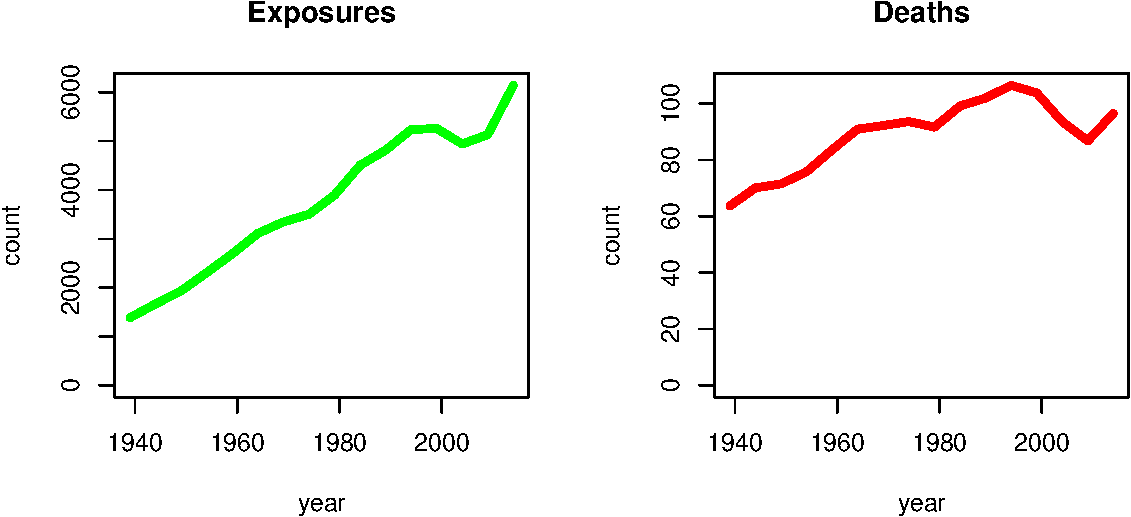
\includegraphics{LifeCon_files/figure-latex/70ChapHMDUSFigsa-1} 

}

\caption{\textbf{Exposures and Deaths (in thousands) for Females age 70 from the HMD U.S.}}\label{fig:70ChapHMDUSFigsa}
\end{figure}

The stark increase in exposures is due to two effects; on one hand, the U.S. population had been growing substantially since 1935, and on the other hand, individuals had been showing an enhanced life expectancy over time. As a consequence, the number of 70-year-old U.S. females had increased from less than two million to more than six million. In contrast, the number of deaths had been more steady. While with an increasing number of exposures the number of deaths have increased, the chance of dying for a 70-year-old had been decreasing. The latter becomes more evident by plotting the ratio of deaths and exposures as in Figure \ref{fig:70DRChapHMDUSFigsa}

R Code For Figure

\hypertarget{toggleCode.70DRChapHMDUSFigs}{}
\begin{Shaded}
\begin{Highlighting}[]
\KeywordTok{par}\NormalTok{(}\DataTypeTok{mfrow=}\KeywordTok{c}\NormalTok{(}\DecValTok{1}\NormalTok{,}\DecValTok{1}\NormalTok{))}
\NormalTok{minlim <-}\StringTok{ }\KeywordTok{min}\NormalTok{(us_deaths[us_deaths}\OperatorTok{$}\NormalTok{Age }\OperatorTok{==}\StringTok{ }\DecValTok{70}\NormalTok{,}\DecValTok{4}\NormalTok{]}\OperatorTok{/}\NormalTok{us_exp[us_exp}\OperatorTok{$}\NormalTok{Age }\OperatorTok{==}\StringTok{ }\DecValTok{70}\NormalTok{,}\DecValTok{4}\NormalTok{])}
\NormalTok{maxlim <-}\StringTok{ }\KeywordTok{max}\NormalTok{(us_deaths[us_deaths}\OperatorTok{$}\NormalTok{Age }\OperatorTok{==}\StringTok{ }\DecValTok{70}\NormalTok{,}\DecValTok{4}\NormalTok{]}\OperatorTok{/}\NormalTok{us_exp[us_exp}\OperatorTok{$}\NormalTok{Age }\OperatorTok{==}\StringTok{ }\DecValTok{70}\NormalTok{,}\DecValTok{4}\NormalTok{])}
\KeywordTok{plot}\NormalTok{(us_deaths[us_deaths}\OperatorTok{$}\NormalTok{Age }\OperatorTok{==}\StringTok{ }\DecValTok{70}\NormalTok{,}\DecValTok{2}\NormalTok{],us_deaths[us_deaths}\OperatorTok{$}\NormalTok{Age }\OperatorTok{==}\StringTok{ }\DecValTok{70}\NormalTok{,}\DecValTok{4}\NormalTok{]}\OperatorTok{/}\NormalTok{us_exp[us_exp}\OperatorTok{$}\NormalTok{Age }\OperatorTok{==}\StringTok{ }\DecValTok{70}\NormalTok{,}\DecValTok{4}\NormalTok{],}\DataTypeTok{type =} \StringTok{"l"}\NormalTok{, }\DataTypeTok{lwd =} \DecValTok{5}\NormalTok{, }\DataTypeTok{col =} \StringTok{"blue"}\NormalTok{, }\DataTypeTok{main=}\StringTok{"Deaths/Exposures"}\NormalTok{, }\DataTypeTok{xlab =} \StringTok{"year"}\NormalTok{, }\DataTypeTok{ylab =} \StringTok{"rate"}\NormalTok{,}\DataTypeTok{ylim =} \KeywordTok{c}\NormalTok{(minlim,maxlim))}
\KeywordTok{rm}\NormalTok{(minlim, maxlim)}
\end{Highlighting}
\end{Shaded}



\begin{figure}

{\centering 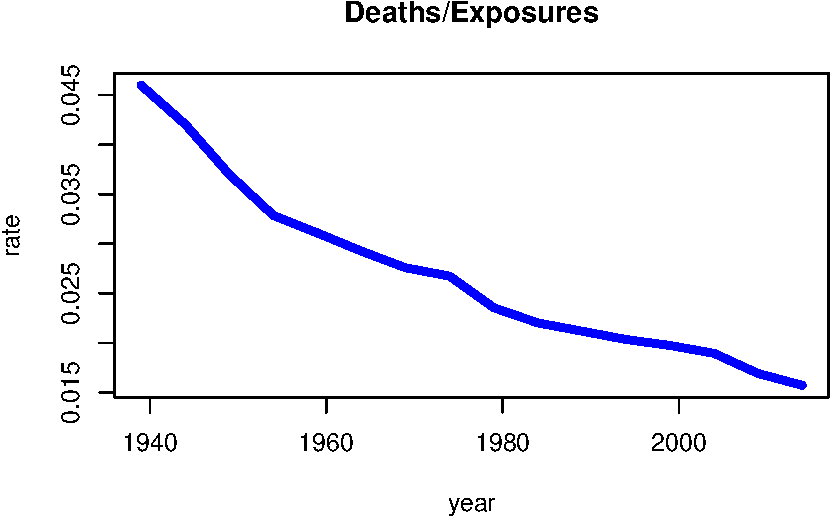
\includegraphics{LifeCon_files/figure-latex/70DRChapHMDUSFigsa-1} 

}

\caption{\textbf{Death rates for Females age 70 from the HMD U.S}}\label{fig:70DRChapHMDUSFigsa}
\end{figure}

Note that the chance of dying for a 70-year-old female was more than 4\% around 1940, but it had decreased over time to a level lower than 2\%. As we will see in Section \ref{S:LifeTab}, the ratio of deaths and exposures is closely related to \emph{death rates}.

Alternatively, we can focus on a specific period -- say the most recent five years in our data, i.e.~2010-2014 -- and plot the deaths over exposures across ages as in Figure \ref{fig:AllDRChapHMDUSFigsa}

R Code For Figure

\hypertarget{toggleCode.AllDRChapHMDUSFigs}{}
\begin{Shaded}
\begin{Highlighting}[]
\NormalTok{us_mx_fem_}\DecValTok{2014}\NormalTok{ <-}\StringTok{ }\NormalTok{us_deaths[us_deaths}\OperatorTok{$}\NormalTok{Year_start }\OperatorTok{==}\StringTok{ }\DecValTok{2010}\NormalTok{,}\DecValTok{4}\NormalTok{]}\OperatorTok{/}\NormalTok{us_exp[us_exp}\OperatorTok{$}\NormalTok{Year_start }\OperatorTok{==}\StringTok{ }\DecValTok{2010}\NormalTok{,}\DecValTok{4}\NormalTok{]}
\NormalTok{us_mx_mal_}\DecValTok{2014}\NormalTok{ <-}\StringTok{ }\NormalTok{us_deaths[us_deaths}\OperatorTok{$}\NormalTok{Year_start }\OperatorTok{==}\StringTok{ }\DecValTok{2010}\NormalTok{,}\DecValTok{5}\NormalTok{]}\OperatorTok{/}\NormalTok{us_exp[us_exp}\OperatorTok{$}\NormalTok{Year_start }\OperatorTok{==}\StringTok{ }\DecValTok{2010}\NormalTok{,}\DecValTok{5}\NormalTok{]}
\KeywordTok{plot}\NormalTok{(us_mx_fem_}\DecValTok{2014}\NormalTok{,}\DataTypeTok{type =} \StringTok{"l"}\NormalTok{, }\DataTypeTok{lwd =} \DecValTok{5}\NormalTok{, }\DataTypeTok{col =} \StringTok{"blue"}\NormalTok{, }\DataTypeTok{main=}\StringTok{"Deaths/Exposures"}\NormalTok{, }\DataTypeTok{xlab =} \StringTok{"year"}\NormalTok{, }\DataTypeTok{ylab =} \StringTok{"death rate"}\NormalTok{, }\DataTypeTok{ylim =} \KeywordTok{c}\NormalTok{(}\KeywordTok{min}\NormalTok{(us_mx_fem_}\DecValTok{2014}\NormalTok{),}\KeywordTok{max}\NormalTok{(us_mx_fem_}\DecValTok{2014}\NormalTok{)))}
\end{Highlighting}
\end{Shaded}



\begin{figure}

{\centering 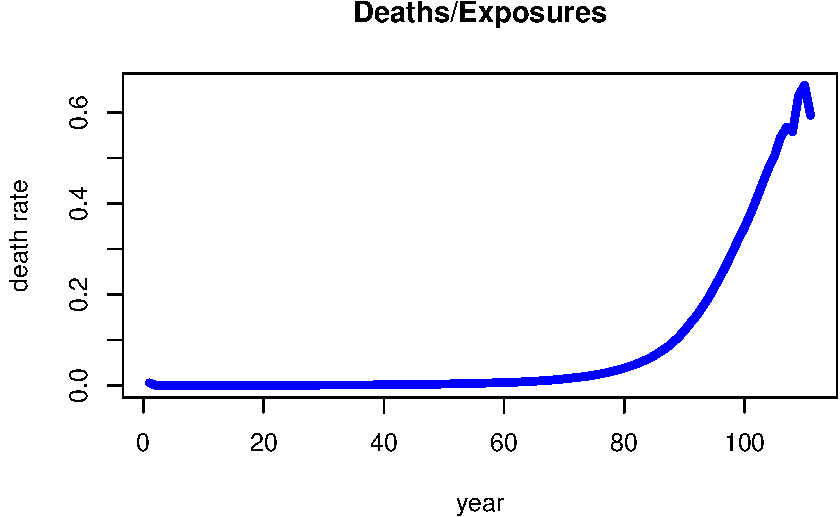
\includegraphics{LifeCon_files/figure-latex/AllDRChapHMDUSFigsa-1} 

}

\caption{\textbf{Death rates for Females across ages for 2010-2014 from the HMD U.S.}}\label{fig:AllDRChapHMDUSFigsa}
\end{figure}

We observe that the death rate increases fairly regularly with respect to age and its growth looks exponential. This observation is the foundation for the most famous and common analytic mortality model that is detailed in Section \ref{S:AnalMortLaws} known as the \emph{Gompertz law}. It should be noted that the death rates at higher ages, specifically from 106 to 110, are showing a larger variability that could be explained by the fact very small sub-populations of high ages are observed and the estimates are more uncertain than those at lower ages.

We note some precaution when using the Human Mortality Database (HMD). It is intended to provide a wide range of interested parties with detailed and up-to-date mortality and population data covering about 41 countries. There are some countries that may exhibit different mortality patterns from these 41 countries, and these include for example, some of the most populous countries such as China, India, and Indonesia, and several countries in the African continents such as South Africa, Nigeria, and Egypt.

\hypertarget{S:IndivMortData}{%
\subsection{Individual Mortality Data}\label{S:IndivMortData}}

While mortality \emph{counts} are a common way to organize mortality data across a large population, which had been our emphasis in the previous section, the individual survival time data may provide valuable pieces of information. Indeed, the data available to an insurance company typically consists of records of individuals. The company records individual details for each insured person from when they purchased the contract; these include personal characteristics such as sex, age, date-of-birth, etc., but also medical records and other \emph{underwriting information}. In addition, the company knows whether or not the person had died at the current time---and if so, the time of death.

This latter aspect is common for \emph{survival} or \emph{event history data}. For each observation (individual) \(i\), a number of covariates or \emph{features} \(\textbf{x}_i\), as well as the \emph{event time} \(T_i\) \emph{if} the event has already happened. Otherwise, we only know that by the current \emph{cutoff} time, the event has not happened yet. In the context of \emph{survival analysis}, which is the branch of statistics that deals with \emph{survival} or \emph{event data}, this is known as \emph{(right) censoring}, i.e.~the data are (right-)censored.

Data protection policies are omnipresent and insurance companies are not any different with respect to policyholder data. On one hand, there are regulatory data protection that disallow disclosure of personal identifiable pieces of information. On the other hand, data are a key resource to a life insurer and sharing this valuable piece of information creates a competition disadvantage by revealing important information to the company's competitive position. Therefore, rather than relying on real survival data, we consider a synthetic dataset consisting of a hypothetical portfolio of policyholders.

In the supplemental information to this text, we provide survival information for a hypothetical insurance company in \texttt{SyntheticInsurerData.csv}. The company has sold ``whole life insurance policies'' for since 1955 (the coming chapters discuss different life insurance policies in detail). Policyholders have to go through an underwriting examination, and in addition to policyholders' age, sex (0 for female, 1 for male), smoking status (0 for non-smoker, 1 for smoker), and the month of sale, the company records the applicants body-mass index (BMI) and the systolic blood pressure at the time of underwriting. Finally, for those policyholders with a claim, i.e., for the policyholders that have died, the company records the time of death (relative to the month of underwriting). The data is organized in the order of sales, so that the oldest entries are at the top of the data and the newest entries are at the bottom:

\begin{Shaded}
\begin{Highlighting}[]
\KeywordTok{library}\NormalTok{(data.table)}
\NormalTok{ins_data <-}\StringTok{ }\KeywordTok{fread}\NormalTok{(}\StringTok{"Data/SyntheticInsurerData.csv"}\NormalTok{,}\DataTypeTok{data.table=}\OtherTok{FALSE}\NormalTok{)}
\KeywordTok{kable}\NormalTok{(}\KeywordTok{head}\NormalTok{(ins_data), }\DataTypeTok{align =} \StringTok{"ccccrrrr"}\NormalTok{,}\DataTypeTok{digits =} \DecValTok{2}\NormalTok{)}
\CommentTok{#displaying the very end of the table similar to the very top of the table requires a few more steps}
\NormalTok{tmp_tail_ins_data <-}\StringTok{ }\KeywordTok{tail}\NormalTok{(ins_data); }\KeywordTok{rownames}\NormalTok{(tmp_tail_ins_data) <-}\StringTok{ }\OtherTok{NULL}
\KeywordTok{kable}\NormalTok{(tmp_tail_ins_data, }\DataTypeTok{align =} \StringTok{"ccccrrrr"}\NormalTok{,}\DataTypeTok{digits =} \DecValTok{2}\NormalTok{)}
\end{Highlighting}
\end{Shaded}

\begin{tabular}{c|c|c|c|r|r|r|r}
\hline
Month\_of\_Sale & Age & Sex & Smoking & BMI & BloodPressure & Claim & Time\_of\_death\\
\hline
1 & 27 & 0 & 0 & 25.8 & 117 & YES & 55.63\\
\hline
1 & 51 & 1 & 0 & 17.6 & 109 & YES & 18.53\\
\hline
1 & 59 & 1 & 0 & 22.5 & 132 & YES & 15.88\\
\hline
1 & 37 & 1 & 0 & 22.9 & 109 & YES & 57.40\\
\hline
1 & 62 & 0 & 0 & 30.9 & 147 & YES & 27.83\\
\hline
1 & 31 & 0 & 0 & 17.3 & 91 & YES & 64.06\\
\hline
\end{tabular}

\begin{tabular}{c|c|c|c|r|r|r|r}
\hline
Month\_of\_Sale & Age & Sex & Smoking & BMI & BloodPressure & Claim & Time\_of\_death\\
\hline
780 & 43 & 0 & 0 & 17.10 & 110 & NO & NA\\
\hline
780 & 57 & 1 & 1 & 19.30 & 118 & NO & NA\\
\hline
780 & 40 & 0 & 0 & 20.10 & 117 & NO & NA\\
\hline
780 & 27 & 1 & 0 & 20.60 & 90 & NO & NA\\
\hline
780 & 55 & 1 & 1 & 20.10 & 118 & NO & NA\\
\hline
780 & 23 & 1 & 0 & 19.03 & 82 & NO & NA\\
\hline
\end{tabular}

Evidently, most of the policies sold in the first months---back in 1955---have matured, and most recently underwritten policyholders are still alive. Let us further investigate the mortality dataframe and we start by summarizing the attributes of our data:

\begin{Shaded}
\begin{Highlighting}[]
\KeywordTok{suppressWarnings}\NormalTok{(}\KeywordTok{library}\NormalTok{(psych))}
\NormalTok{tmp_describe_ins_data<-psych}\OperatorTok{::}\KeywordTok{describe}\NormalTok{(ins_data)}
\KeywordTok{kable}\NormalTok{(tmp_describe_ins_data, }\DataTypeTok{digits =} \DecValTok{2}\NormalTok{, }\DataTypeTok{format.args =} \KeywordTok{list}\NormalTok{(}\DataTypeTok{big.mark =} \StringTok{","}\NormalTok{))}
\end{Highlighting}
\end{Shaded}

\begin{tabular}{l|r|r|r|r|r|r|r|r|r|r|r|r|r}
\hline
  & vars & n & mean & sd & median & trimmed & mad & min & max & range & skew & kurtosis & se\\
\hline
Month\_of\_Sale & 1 & 160,781 & 394.58 & 216.72 & 382.00 & 393.08 & 277.25 & 1.0 & 780.0 & 779.0 & 0.08 & -1.17 & 0.54\\
\hline
Age & 2 & 160,781 & 39.99 & 11.61 & 39.00 & 39.65 & 11.86 & 19.0 & 65.0 & 46.0 & 0.22 & -0.73 & 0.03\\
\hline
Sex & 3 & 160,781 & 0.70 & 0.46 & 1.00 & 0.75 & 0.00 & 0.0 & 1.0 & 1.0 & -0.87 & -1.25 & 0.00\\
\hline
Smoking & 4 & 160,781 & 0.30 & 0.46 & 0.00 & 0.25 & 0.00 & 0.0 & 1.0 & 1.0 & 0.88 & -1.22 & 0.00\\
\hline
BMI & 5 & 160,781 & 22.79 & 4.55 & 21.70 & 22.20 & 3.85 & 16.1 & 69.6 & 53.5 & 1.46 & 3.26 & 0.01\\
\hline
BloodPressure & 6 & 160,781 & 114.74 & 15.75 & 114.00 & 114.36 & 16.31 & 57.0 & 208.0 & 151.0 & 0.26 & 0.09 & 0.04\\
\hline
Claim* & 7 & 160,781 & 1.37 & 0.48 & 1.00 & 1.34 & 0.00 & 1.0 & 2.0 & 1.0 & 0.54 & -1.71 & 0.00\\
\hline
Time\_of\_death & 8 & 59,382 & 28.27 & 13.69 & 28.36 & 28.24 & 15.21 & 0.0 & 64.2 & 64.2 & 0.02 & -0.73 & 0.06\\
\hline
\end{tabular}

In summary, there are 160,781 insureds, out of which 59,382, i.e.~36.93\%, have died; the average age at purchase is about 40, and our portfolio has a high percentage of men (70\%) and non-smokers (70\%). The average BMI is 22.8 and the average blood pressure is 114.7, which are close to (but somewhat lower than) U.S. national averages; for details on common BMI and blood pressure levels, see e.g.~the \href{https://obs.withings.com/us}{Withings Health Observatory} that provides real-time information for U.S. Americans.

To illustrate the sales history, we plot the monthly sales of the company, which is given as Figure \ref{fig:MonthlySalesFigsa}.

R Code For Figure

\hypertarget{toggleCode.MonthlySalesFigs}{}
\begin{Shaded}
\begin{Highlighting}[]
\NormalTok{monthly_sales <-}\StringTok{ }\KeywordTok{rep}\NormalTok{(}\DecValTok{0}\NormalTok{,}\DecValTok{780}\NormalTok{)}
\ControlFlowTok{for}\NormalTok{ (i }\ControlFlowTok{in} \DecValTok{1}\OperatorTok{:}\DecValTok{780}\NormalTok{)\{}
\NormalTok{  monthly_sales[i] <-}\StringTok{ }\KeywordTok{sum}\NormalTok{(ins_data}\OperatorTok{$}\NormalTok{Month_of_Sale }\OperatorTok{==}\StringTok{ }\NormalTok{i)}
\NormalTok{\}}
\KeywordTok{plot}\NormalTok{(monthly_sales,}\DataTypeTok{type =} \StringTok{"l"}\NormalTok{, }\DataTypeTok{lwd =} \DecValTok{2}\NormalTok{, }\DataTypeTok{col =} \StringTok{"green"}\NormalTok{, }\DataTypeTok{main=}\StringTok{"Monthly Sales"}\NormalTok{, }\DataTypeTok{xlab =} \StringTok{"month"}\NormalTok{, }\DataTypeTok{ylab =} \StringTok{"Sales"}\NormalTok{)}
\KeywordTok{abline}\NormalTok{(}\DataTypeTok{h =} \KeywordTok{mean}\NormalTok{(monthly_sales), }\DataTypeTok{col =} \StringTok{"red"}\NormalTok{, }\DataTypeTok{lty =} \DecValTok{2}\NormalTok{)}
\end{Highlighting}
\end{Shaded}



\begin{figure}

{\centering 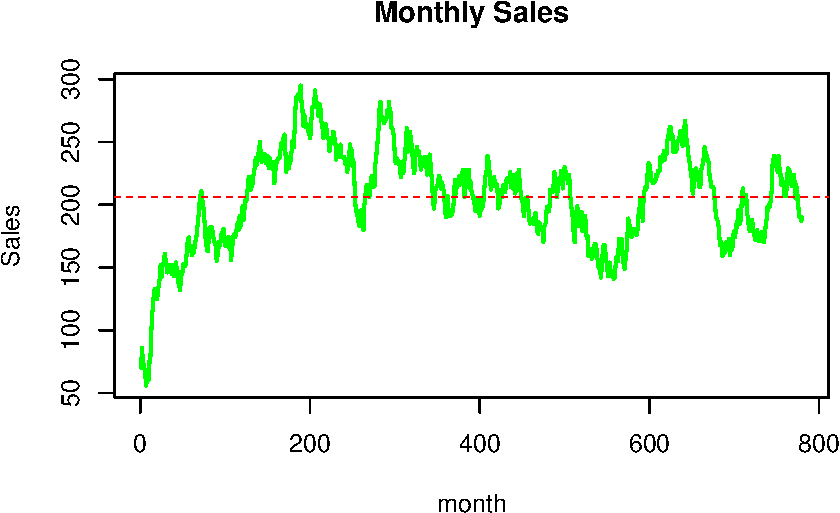
\includegraphics{LifeCon_files/figure-latex/MonthlySalesFigsa-1} 

}

\caption{\textbf{Monthy sales for the synthetic mortality data}}\label{fig:MonthlySalesFigsa}
\end{figure}

In summary, the company sells about 200 insurance contracts each month, although there is some variation over time; while sales initially increased, the company experience some ebbs and flows, potentially due to marketing efforts and/or the effectiveness or attractiveness of the products.

We now investigate the traits of the insureds for which various histograms are given as Figure \ref{fig:HistInsDataFigsa}.

R Code For Figure

\hypertarget{toggleCode.HistInsDataFigs}{}
\begin{Shaded}
\begin{Highlighting}[]
\KeywordTok{par}\NormalTok{(}\DataTypeTok{mfrow=}\KeywordTok{c}\NormalTok{(}\DecValTok{1}\NormalTok{,}\DecValTok{3}\NormalTok{))}
\KeywordTok{hist}\NormalTok{(ins_data}\OperatorTok{$}\NormalTok{Age,}\DataTypeTok{main=}\StringTok{"Insured Age"}\NormalTok{, }\DataTypeTok{xlab=}\StringTok{"age"}\NormalTok{, }\DataTypeTok{border=}\StringTok{"red"}\NormalTok{, }\DataTypeTok{col=}\StringTok{"green"}\NormalTok{)}
\KeywordTok{hist}\NormalTok{(ins_data}\OperatorTok{$}\NormalTok{BMI,}\DataTypeTok{main=}\StringTok{"Body Mass Index"}\NormalTok{, }\DataTypeTok{xlab=}\StringTok{"bmi"}\NormalTok{, }\DataTypeTok{border=}\StringTok{"red"}\NormalTok{, }\DataTypeTok{col=}\StringTok{"green"}\NormalTok{)}
\KeywordTok{hist}\NormalTok{(ins_data}\OperatorTok{$}\NormalTok{BloodPressure,}\DataTypeTok{main=}\StringTok{"Systolic Blood Pressure"}\NormalTok{, }\DataTypeTok{xlab=}\StringTok{"bp"}\NormalTok{, }\DataTypeTok{border=}\StringTok{"red"}\NormalTok{, }\DataTypeTok{col=}\StringTok{"green"}\NormalTok{)}
\end{Highlighting}
\end{Shaded}



\begin{figure}

{\centering 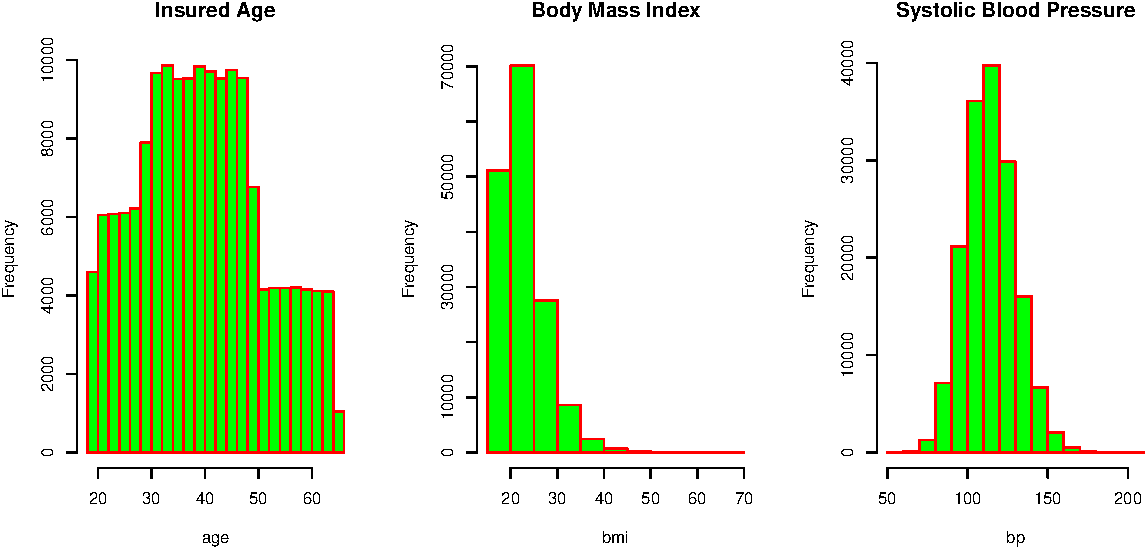
\includegraphics{LifeCon_files/figure-latex/HistInsDataFigsa-1} 

}

\caption{\textbf{Histograms for the synthetic mortality data}}\label{fig:HistInsDataFigsa}
\end{figure}

Most individuals are in between thirty and fifty years of age when purchasing the coverage, but some sales to younger and some older individuals are observed. The \emph{Body Mass Index (BMI)} is concentrated between 20 and 30, although there are some outliers with relatively large values. The systolic blood pressure is roughly bell shaped, with most applicants exhibiting blood pressure measurements at normal levels (below 120) or slightly elevated levels (120-130). We further visualize the relationship between these three attributes by looking at the correlation correlation matrix corresponding to these three characteristics, which is given as Figure \ref{fig:CorrPlotInsDataFigsa}.

R Code For Figure

\hypertarget{toggleCode.CorrPlotInsDataFigs}{}
\begin{Shaded}
\begin{Highlighting}[]
\KeywordTok{suppressWarnings}\NormalTok{(}\KeywordTok{library}\NormalTok{(corrplot))}
\NormalTok{tmp_corr_ins_data <-}\StringTok{ }\KeywordTok{cor}\NormalTok{(ins_data[,}\KeywordTok{c}\NormalTok{(}\DecValTok{2}\NormalTok{,}\DecValTok{5}\NormalTok{,}\DecValTok{6}\NormalTok{)])}
\KeywordTok{colnames}\NormalTok{(tmp_corr_ins_data) <-}\StringTok{ }\KeywordTok{c}\NormalTok{(}\StringTok{"Age"}\NormalTok{, }\StringTok{"BMI"}\NormalTok{, }\StringTok{"BP"}\NormalTok{)}
\KeywordTok{rownames}\NormalTok{(tmp_corr_ins_data) <-}\StringTok{ }\KeywordTok{c}\NormalTok{(}\StringTok{"Age"}\NormalTok{, }\StringTok{"BMI"}\NormalTok{, }\StringTok{"BP"}\NormalTok{)}
\KeywordTok{corrplot}\NormalTok{(tmp_corr_ins_data, }\DataTypeTok{method=}\StringTok{"circle"}\NormalTok{, }\DataTypeTok{order=}\StringTok{"hclust"}\NormalTok{, }\DataTypeTok{addCoef.col =} \StringTok{"red"}\NormalTok{, }\DataTypeTok{tl.col=}\StringTok{"black"}\NormalTok{,}\DataTypeTok{tl.srt=}\DecValTok{45}\NormalTok{)}
\end{Highlighting}
\end{Shaded}



\begin{figure}

{\centering 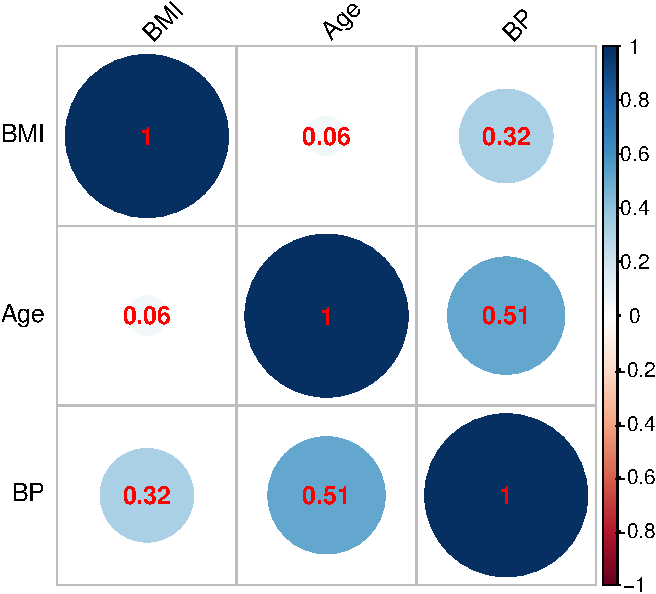
\includegraphics{LifeCon_files/figure-latex/CorrPlotInsDataFigsa-1} 

}

\caption{\textbf{Correlation matrix for the synthetic mortality data corresponding to age, BMI and BP (blood pressure)}}\label{fig:CorrPlotInsDataFigsa}
\end{figure}

Clearly, high blood pressure and elevated BMI are positively associated, and an elevated blood pressure is more common for elderly insureds, which are common observations in many populations.

One of our main focus is the realized lifetime, which can only be observed for those individuals where a claim had been paid. We thus plot the distribution of the age at death based on these observations, which is illustrated in Figure \ref{fig:AgeDeathHistInsDataFigs}.

\begin{Shaded}
\begin{Highlighting}[]
\KeywordTok{hist}\NormalTok{(ins_data}\OperatorTok{$}\NormalTok{Age}\OperatorTok{+}\NormalTok{ins_data}\OperatorTok{$}\NormalTok{Time_of_death,}\DataTypeTok{main=}\StringTok{"Age at Death"}\NormalTok{, }\DataTypeTok{xlab=}\StringTok{"age"}\NormalTok{, }\DataTypeTok{border=}\StringTok{"red"}\NormalTok{, }\DataTypeTok{col=}\StringTok{"green"}\NormalTok{)}
\end{Highlighting}
\end{Shaded}

\begin{figure}

{\centering 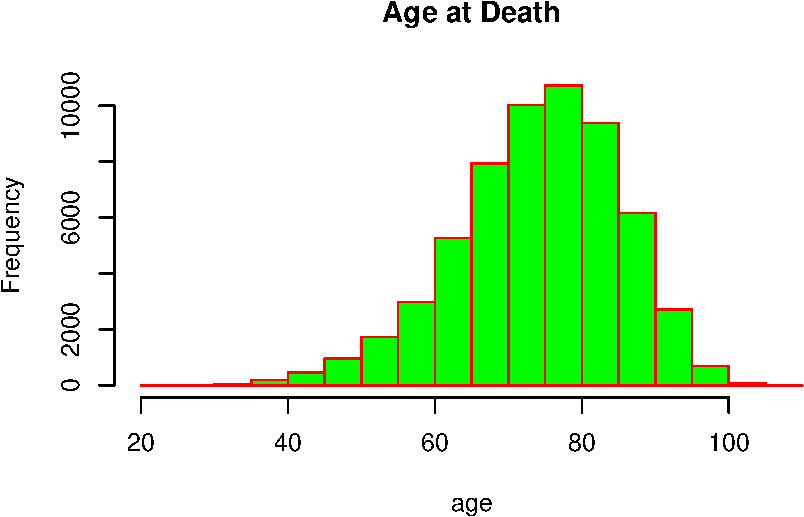
\includegraphics{LifeCon_files/figure-latex/AgeDeathHistInsDataFigs-1} 

}

\caption{Age at Death for the synthetic mortality data}\label{fig:AgeDeathHistInsDataFigs}
\end{figure}

Not surprisingly, the majority of deceased policyholders have died at higher ages, since the bulk of deaths are concentrated between seventy and ninety years old. There are a few individuals that died relatively young, and similarly a few that were close to achieving the centenarian status, though it should be noted that some policyholders at higher ages may still be alive. Indeed, the ages of five oldest individuals that are still alive are

\begin{Shaded}
\begin{Highlighting}[]
\KeywordTok{round}\NormalTok{(}\KeywordTok{tail}\NormalTok{(}\KeywordTok{sort}\NormalTok{(ins_data[ins_data}\OperatorTok{$}\NormalTok{Claim }\OperatorTok{==}\StringTok{ "NO"}\NormalTok{,}\DecValTok{2}\NormalTok{]}\OperatorTok{+}\StringTok{ }\NormalTok{(}\DecValTok{780} \OperatorTok{-}\StringTok{ }\NormalTok{ins_data[ins_data}\OperatorTok{$}\NormalTok{Claim }\OperatorTok{==}\StringTok{ "NO"}\NormalTok{,}\DecValTok{1}\NormalTok{])}\OperatorTok{/}\DecValTok{12}\NormalTok{),}\DecValTok{5}\NormalTok{), }\DataTypeTok{digits =} \DecValTok{2}\NormalTok{)}
\end{Highlighting}
\end{Shaded}

\begin{verbatim}
[1] 102.50 102.67 103.50 104.17 105.58
\end{verbatim}

and thus, it is clear that we observe not many centenarians.

It is intuitive that the number of deaths are associated with sales: The maximal number of deaths is the number of individuals that purchased insurance. This is evident when plotting the number of deaths by the year of sale, which is displayed in Figure \ref{fig:DeathSalesPlotInsDataFigsa}, particularly over the early years.

R Code For Figure

\hypertarget{toggleCode.DeathSalesPlotInsDataFigs}{}
\begin{Shaded}
\begin{Highlighting}[]
\NormalTok{annual_death <-}\StringTok{ }\KeywordTok{rep}\NormalTok{(}\DecValTok{0}\NormalTok{,}\DecValTok{65}\NormalTok{)}
\ControlFlowTok{for}\NormalTok{ (i }\ControlFlowTok{in} \DecValTok{1}\OperatorTok{:}\DecValTok{65}\NormalTok{)\{}
  \ControlFlowTok{for}\NormalTok{ (j }\ControlFlowTok{in} \DecValTok{1}\OperatorTok{:}\DecValTok{12}\NormalTok{)\{}
\NormalTok{    annual_death[i] <-}\StringTok{ }\NormalTok{annual_death[i] }\OperatorTok{+}\StringTok{ }\KeywordTok{sum}\NormalTok{(ins_data[ins_data}\OperatorTok{$}\NormalTok{Month_of_Sale }\OperatorTok{==}\StringTok{ }\NormalTok{(i}\DecValTok{-1}\NormalTok{)}\OperatorTok{*}\DecValTok{12} \OperatorTok{+}\NormalTok{j,}\DecValTok{7}\NormalTok{] }\OperatorTok{==}\StringTok{ "YES"}\NormalTok{) }
\NormalTok{  \}}
\NormalTok{\}}
\KeywordTok{plot}\NormalTok{(annual_death,}\DataTypeTok{type =} \StringTok{"l"}\NormalTok{, }\DataTypeTok{lwd =} \DecValTok{4}\NormalTok{, }\DataTypeTok{col =} \StringTok{"blue"}\NormalTok{, }\DataTypeTok{main=}\StringTok{"Annual Deaths"}\NormalTok{, }\DataTypeTok{xlab =} \StringTok{"Year"}\NormalTok{, }\DataTypeTok{ylab =} \StringTok{"Deaths"}\NormalTok{)}
\end{Highlighting}
\end{Shaded}



\begin{figure}

{\centering 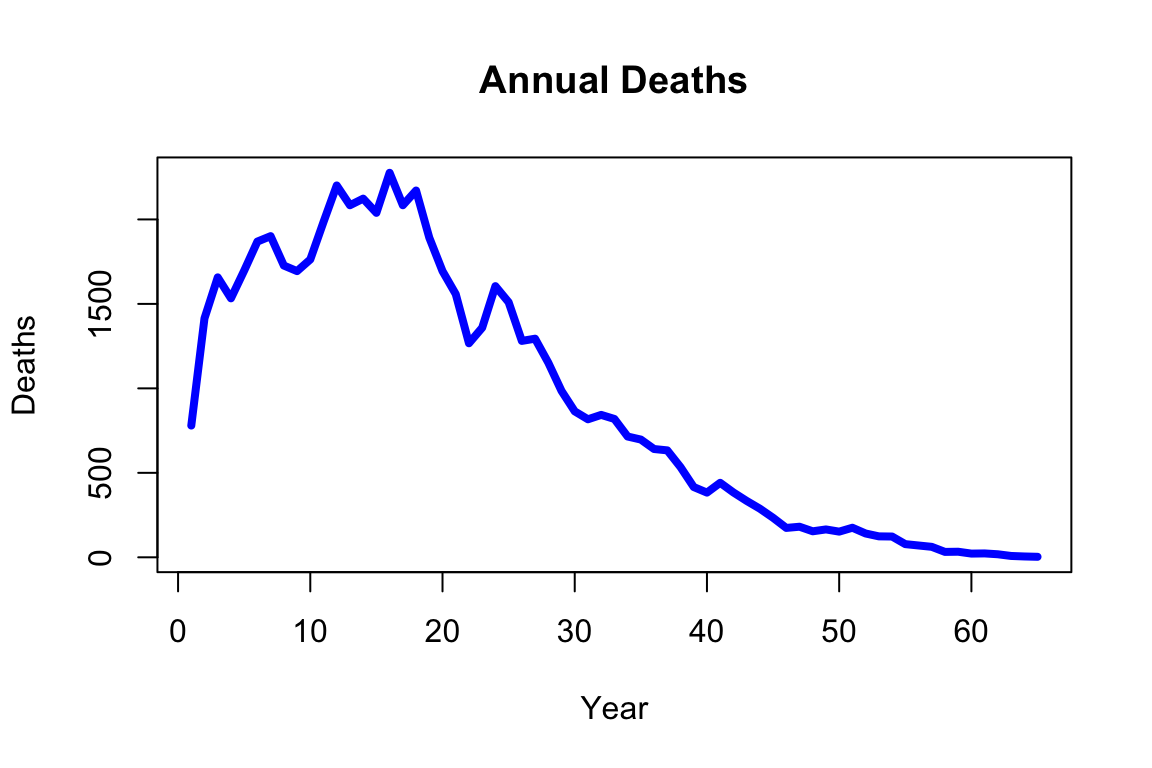
\includegraphics{LifeCon_files/figure-latex/DeathSalesPlotInsDataFigsa-1} 

}

\caption{\textbf{Annual deaths for the synthetic mortality data}}\label{fig:DeathSalesPlotInsDataFigsa}
\end{figure}

We can also investigate the relationship of the time of death to policyholder characteristics by creating a correlation plot amongst those that had already died. The correlation matrix appears as Figure \ref{fig:DeadCorrPlotInsDataFigsa}.

R Code For Figure

\hypertarget{toggleCode.DeadCorrPlotInsDataFigs}{}
\begin{Shaded}
\begin{Highlighting}[]
\CommentTok{#suppressWarnings(library(corrplot))}
\NormalTok{tmp_dead_corr_ins_data <-}\StringTok{ }\KeywordTok{cor}\NormalTok{(ins_data[ins_data}\OperatorTok{$}\NormalTok{Claim }\OperatorTok{==}\StringTok{ "YES"}\NormalTok{,}\KeywordTok{c}\NormalTok{(}\DecValTok{2}\NormalTok{,}\DecValTok{5}\NormalTok{,}\DecValTok{6}\NormalTok{,}\DecValTok{8}\NormalTok{)])}
\KeywordTok{colnames}\NormalTok{(tmp_dead_corr_ins_data) <-}\StringTok{ }\KeywordTok{c}\NormalTok{(}\StringTok{"Age"}\NormalTok{, }\StringTok{"BMI"}\NormalTok{, }\StringTok{"BP"}\NormalTok{, }\StringTok{"TD"}\NormalTok{)}
\KeywordTok{rownames}\NormalTok{(tmp_dead_corr_ins_data) <-}\StringTok{ }\KeywordTok{c}\NormalTok{(}\StringTok{"Age"}\NormalTok{, }\StringTok{"BMI"}\NormalTok{, }\StringTok{"BP"}\NormalTok{, }\StringTok{"TD"}\NormalTok{)}
\KeywordTok{corrplot}\NormalTok{(tmp_dead_corr_ins_data, }\DataTypeTok{method=}\StringTok{"circle"}\NormalTok{, }\DataTypeTok{order=}\StringTok{"hclust"}\NormalTok{, }\DataTypeTok{addCoef.col =} \StringTok{"red"}\NormalTok{, }\DataTypeTok{tl.col=}\StringTok{"black"}\NormalTok{, }\DataTypeTok{tl.srt=}\DecValTok{45}\NormalTok{)}
\end{Highlighting}
\end{Shaded}



\begin{figure}

{\centering 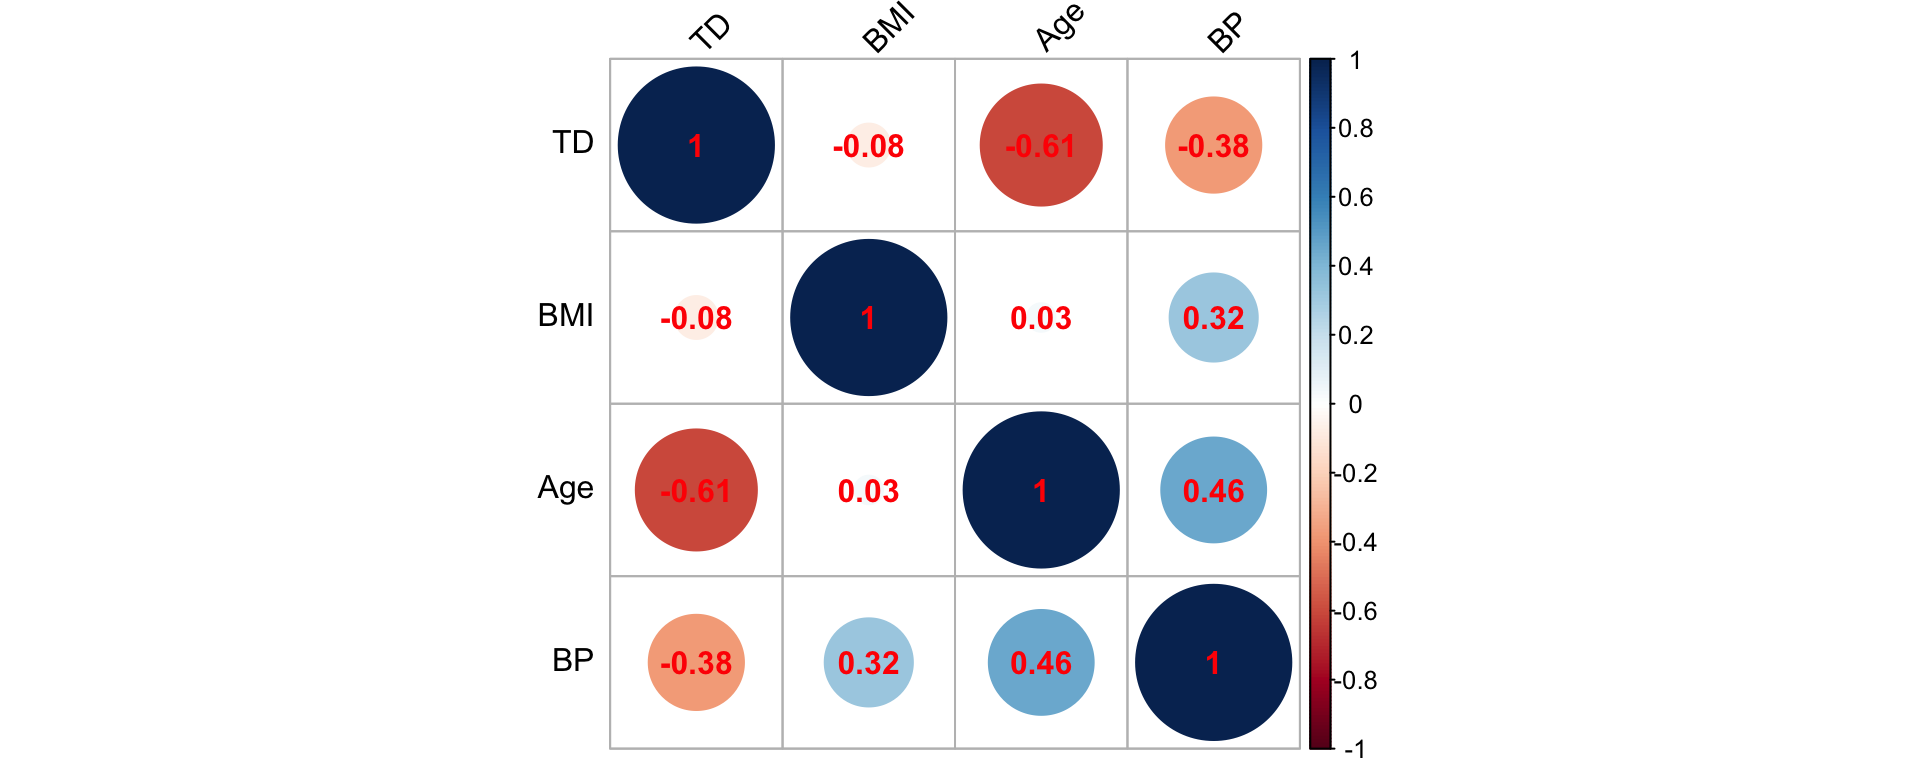
\includegraphics{LifeCon_files/figure-latex/DeadCorrPlotInsDataFigsa-1} 

}

\caption{\textbf{Correlation matrix for the synthetic mortality data corresponding to age, BMI, BP (blood pressure) and TD (time of death)}}\label{fig:DeadCorrPlotInsDataFigsa}
\end{figure}

Hence, the time of death is (strongly) negatively associated with age, which is not surprising as elderly individuals are more likely to die. Similar behaviour is also observed for the BMI and blood pressure attributes that are negatively associated with the the time of death, but we should clarify that the BMI and blood pressure measurements are observed at policy inception though these negative associations explain why such attributes are good predictors of the insured's health. The pairwise correlation between age, BMI and blood pressure are in line with our findings from Figure \ref{fig:CorrPlotInsDataFigsa} that includes all insureds irrespective of their life status.

Even this simple analysis helps in understanding why the life office should evaluate the individual risk per policy by taking into consideration the available information, and more importantly, to have a fair evaluation of the covariates with strong influence over the policy final payout.

Returning to our general description of survival data sets in the current context, if there was a claim and the death event was recorded, this data entry is \emph{non-censored}; however, if the claim is not raised, then the policyholder is alive by the end of the observation period, and in turn, this datum is \emph{right-censored} as the death event has not yet occurred. For example, a policyholder of age \(33\) buys a policy in early January 1990, i.e.~her/his \emph{Month\_of\_Sale} record would be \(421\) -- recall that month \(780\) indicates that a policy is bought in December 2019. If the policyholder survives by the end of the observation period, then a censored datum is recorded as \(30\); in contrast, if the policyholder dies 13 years and 2 months after, then a censored datum is recorded with an event time \(13+2/12\approx13.17\).

\hypertarget{Sec:ModelingDeaths}{%
\section{Modeling Death}\label{Sec:ModelingDeaths}}

The previous section has introduced various examples of mortality data. Clearly, the most relevant question to actuaries is how to use the available pieces of information in order to devise lifetime models that could become the basis for analyzing the life contingent exposures. This section provides the theoretical foundation for modeling lifetimes.

An important caveat is that we focus, both in the presentation of the datasets and in the modeling considerations in this chapter, on understanding the \emph{lifetime uncertainty} for a given individual or (sub)population, where the life status is assumed to be dichotomous, i.e.~\emph{alive} and \emph{dead} are the only life status under observation. Clearly, this simplified assumption helps us to create a parsimonious presentation that is fit for its purpose at this very moment, though one could consider \emph{multi-state models} -- with multiple life status such as alive, death, temporary disability, permanent disability and any other long term health condition, etc. -- or \emph{models with multiple decrements} that relate to specific life insurance products where the modeler could consider non-health related factors such as early termination of a contract that have an impact on the policy's cashflows. Clearly multi-state and multi-decrement models present a generalization of the dichotomous lifetime model, where there are only two states -- alive and dead -- and a single decrement -- dying, respectively. However, aside from being an important special case, there are benefits to discussing and building such more general models armed with the understanding of and experience working with the dichotomous model. We will return to multi-decrement and multi-state models in Chapter XX.

We commence by introducing the most important concept of a lifetime random variable and then discuss key actuarial quantities that allow for a formal interpretation of the data previously presented. We deviate from a traditional actuarial presentation in that we allow for general attributes, which we denote by \(\bf{x}\), to affect the lifetime distribution. However, towards the end of the section, we specialize to the more limited -- but in traditional actuarial modeling conventional
-- assumption that the only relevant (dynamic) covariate for the distribution of the lifetimes is age \(x\).

\hypertarget{lifetime-random-variable-and-its-distribution}{%
\subsection{Lifetime Random Variable and its Distribution}\label{lifetime-random-variable-and-its-distribution}}

We start by considering an individual with attributes \(\bf{x}\) from some feature space. We assume that the attributes \(\bf{x}\) are sufficient to determine the distribution of the individual's future lifetime, which we denote by \(T_{\bf{x}}\). In other words, the \emph{lifetime random variable} \(T_{\bf{x}}\) follows a distribution depending on the attributes \(\bf{x}\). We will assume this random variable has positive real values, i.e.~its support is \((0,\infty)\), and that the random variable is ``well-behaved'' (integrable, continuous, etc.) so that all the operations in what follows are well-defined.

It is helpful to pause and reflect on different types of possible attributes. Some attributes, such as the individual's race, the individual's (biological) sex, race, learned profession, etc., are immutable. Thus, one can either include them in the considered set of attributes \(\bf{x}\). \emph{Or} we can consider a population of individuals with the same immutable characteristics, and then differentiate them solely by non-immutable characteristics \(\bf{x}\). An example are the life expectancy tables in Section \ref{S:DataLifeExp}: here the relevant population could be hispanic females, for which we distinguished (only) different age levels. This approach, where \emph{age} -- typically denoted by \(x\) -- is the only attribute under consideration, is the setting contemplated in traditional life-contingent analysis, and we will discuss this as an important special case in the last part \ref{S:ModelOnlyAge} of this section.

However, the latter setting is restrictive from a number of perspectives. For instance, there are various individual characteristics that are relevant to the future lifetime that are non-immutable. For instance, the health-related attributes of BMI and systolic blood pressure in the dataset presented in Section \ref{S:IndivMortData} may change over time, and a blood pressure level of 130 for a 30 year old may carry a different interpretation than a level of 130 for a 70 year old. Moreover, environmental or socio-economic conditions may change over time and could impact the distribution of future lifetimes, and these could also be reflected in the set of attributes \(\bf{x}\). We leave the exploration of different relevant examples to the remaining sections of this chapter as well as later, more advanced chapters of this book.

Let \(F_{\bf{x}}\) and \(S_{\bf{x}}\) be the \emph{cumulative distribution function} (cdf) and \emph{survival function} of \(T_{\bf{x}}\), respectively:
\[
F_{\bf{x}}(t) =\Pr(T_{\bf{x}}\le t)\quad \text{and}\quad S_{\bf{x}}(t) =\Pr(T_{\bf{x}} > t)=1-\Pr(T_{\bf{x}} \le t)=1-F_{\bf{x}}(t)\quad\text{for all}\;t\geq0.
\]

Given our natural assumption that the lifetime variable \(T_{\bf{x}}\) is continuously distributed, i.e.~that there are no outcomes that carry point masses, we can also defined its probability density function \(f_{\bf{x}}\):

\[
f_{\bf{x}}(t) =\frac{\partial F_{\bf{x}}(t)}{\partial t}=\frac{\partial \big(1- S_{\bf{x}}(t)\big)}{\partial t}=-\frac{\partial S_{\bf{x}}(t)}{\partial t},\;t\geq 0.
\]

Similarly, we can define the \emph{force of mortality}, \(\mu_\bf{x}\), which in different contexts is also referred to as the \emph{hazard rate} or the \emph{mortality intensity}:

\[
\mu_{\bf{x}}(t) = - \frac{\partial \log\{ S_{\bf{x}}(t)\}}{\partial t} = \frac{-\frac{\partial S_{\bf{x}}(t)}{\partial t}}{S_{\bf{x}}(t)}=\frac{f_{\bf{x}}(t)}{S_{\bf{x}}(t)},\;t\geq 0,
\]

which is equivalent to:
\[
S_{\bf{x}}(t) = \exp\left\{-\int_0^t \mu_{\bf{x}}(s)\;ds \right\}\quad\text{for all}\quad t\ge 0.
\]
The important point to note is that any one of the functions \(F_{\bf{x}}\), \(S_{\bf{x}}\), \(f_{\bf{x}}\), or \(\mu_{\bf{x}}\) completely determines the distribution of the future lifetime \(T_{\bf{x}}\). In other words, in order to specify a probabilistic model of future lifetimes, we can choose to model any of these quantities -- knowing the form of just one of them will allow you to determine expressions for the other functions.

\hypertarget{standard-actuarial-notation-q_bfx-_tp_bfx-and-all-that}{%
\subsection{\texorpdfstring{Standard Actuarial Notation: \(q_{\bf{x}}\), \(_tp_{\bf{x}}\), and All That}{Standard Actuarial Notation: q\_\{\textbackslash bf\{x\}\}, \_tp\_\{\textbackslash bf\{x\}\}, and All That}}\label{standard-actuarial-notation-q_bfx-_tp_bfx-and-all-that}}

The introduction of the lifetime random variable, in principle, is enough for actuarial analyses of life-contingent exposures. In particular, as we will see in the next chapter, based on \(T_{\bf{x}}\) we can model (discounted) cash flows of common life insurance and annuity products, determine their expected values and variances, etc. However, the discussion so far was primarily formal and did not instill much intuition. For instance, the cdf \(F_{\bf{x}}(t)\) at time \(t\) is nothing else than the probability that an individual will die before a certain time \(t\), i.e.~the \emph{mortality probability}; and the expected value of \(T_{\bf{x}}\) is nothing else than the expected years lived, i.e.~the \emph{life expectancy}, for an individual with attributes \(\bf{x}\) that we had already encountered in Section \ref{S:DataLifeExp} in the context of national vital statistics.

To instill interpretation into the notation, but also to have a precise, uniform representation to record and communicate relevant quantities, actuaries around the globe rely on so-called \href{https://en.wikipedia.org/wiki/Actuarial_notation}{standard actuarial notation}. This notation is based on a so-called \emph{Halo} system where symbols are placed as superscript or subscript before or after a main character. In particular, the \(t\)-year \emph{mortality probability} for an individual with attributes \(\bf{x}\) is denotes by \(_tq_{\bf{x}}\):
\[
{_tq_{\bf{x}}} = F_{\bf{x}}(t),\;t\geq 0.
\]
Similarly the \(t\)-year \emph{survival probability}, denoted by \(_tp_{\bf{x}}\), is nothing else than the survival function:
\[
{_tp_{\bf{x}}} = S_{\bf{x}}(t),\;t\geq 0.
\]
Clearly, \({_tp_{\bf{x}}}+{_tq_{\bf{x}}}=1\), since the individual \(x\) either dies or survives after \(t\) units of time. Furthermore, is is conventional to drop a superscript of one:
\[
{_1p_{\bf{x}}} = {p_{\bf{x}}}\quad\text{and}\quad {_1q_{\bf{x}}} = {q_{\bf{x}}}.
\]
Furthemore, we denote the \(s\)-year mortality probability after surviving for \(t\) years as:
\[
{_{t|s}q_{\bf{x}}} = F_{\bf{x}}(t+s) - F_{\bf{x}}(t) = {_{t+s}q_{\bf{x}}} - {_tq_{\bf{x}}} = S_{\bf{x}}(t) - S_{\bf{x}}(t+s) = {_tp_{\bf{x}}} - {_{t+s}p_{\bf{x}}} ,\;t,s\geq 0.
\]

As indicated, the expected value of the lifetime random variable corresponds to the \emph{(complete) expectation of life} or \emph{life expectancy}. It is defined as follows:

\[
\stackrel{\circ}{e}_{\bf{x}}=E[T_{\bf{x}}]=\int_0^\infty t \,f_{\bf{x}}(t)\;dt=\int_0^\infty {_tp_{\bf{x}}}\;dt,
\]
where the last equaility follows from integration by parts.

Derivation of Formula for Complete Life Expectancy

\leavevmode\hypertarget{toggleTheory.DerivationLifeExp}{}%
\[
\stackrel{\circ}{e}_{\bf{x}} = E[T_{\bf{x}}] = \int_0^{\infty} t\, \underbrace{f_{\bf{x}}(t)}_{-S_{\bf{x}}'(t)}\,dt = - \left[S_{\bf{x}}(t)\, t\right]_{t=0}^{\infty} + \int_0^{\infty} S_{\bf{x}}(t)\,dt = \int_0^{\infty} {_tp_{\bf{x}}}\,dt.
\]

It is also helpful to define a \emph{temporary} version of the expectation of life, i.e.~the number of years lived wihin the next \(n\) years. In actuarial notation, temporary quantities are denoted by \(\cdot_{\cdot:\overline{n}|}\):
\[
\stackrel{\circ}{e}_{{\bf{x}}:\overline{n}|} = E[\min\{T_{\bf{x}},n\}] = \int_0^{n} {_tp_{\bf{x}}}\,dt.
\]
The interpretation is that unlike for the complete expectation of life, we only count years lived until time \(n.\) For instance, considering a population of \(l_0\) individuals, while \(l_0 \times {_tp_{\bf{x}}}\) denotes the expected number of survivors until time \(t\), \(l_0 \times \stackrel{\circ}{e}_{{\bf{x}}:\overline{t}|}\) denotes the average size of the population over the next \(t\) periods. We will return to this point in the context of life tables in section \ref{S:LifeTab}.

We will see many more examples of actuarial notation through the course of this book, and we will heavily rely on it.

\hypertarget{S:ModelOnlyAge}{%
\subsection{The Classical Case: Age-Only Model}\label{S:ModelOnlyAge}}

As mentioned, an important special case is the situation where the only (non-immutable) attribute is age. In this case, it is conventional to write \({\bf{x}} = x\), where \(x\) is a number denoting current age, and the lifetime random variable \(T_x\) that explains the remaining future lifetime for an individual currently aged \(x\). Hence, in this case, \(T_x\) -- and its distribution -- solely depends on the age \(x\), and, thus, \(T_x\) and \(T_0|T_0>x\) are identically distributed random variables (here \(T_0|T_0>x\) denotes the random variable conditional on the event \(\{T_0>x\}\)). In other words, the future lifetime for \((x)\) is the same as the future lifetime of a newborn given that this newborn reaches age \(x\), \(T_0>x\).

The mathematical formulations are thus described by conditional probabilities:
\begin{eqnarray*}
{_tq_x} = F_x(t) &=& Pr(T_x \le t) = Pr(T_x \le t \mid T_x>0) \\
&=& Pr(T_0-x \le t \mid T_0-x>0) = Pr(T_0 \le x + t \mid T_0 > x)\\
&=&\frac{\Pr(x<T_0\leq x+t)}{\Pr(T_0>x)}=\frac{F_0(x+t)-F_0(x)}{S_0(x)}=\frac{S_0(x)-S_0(x+t)}{S_0(x)}
\end{eqnarray*}
and
\begin{eqnarray*}
{_tp_x} = S_x(t) &=& Pr(T_x > t) = Pr(T_x > t \mid T_x > 0) \\
&=& Pr(T_0-x > t \mid T_0-x>0) =  Pr(T_0 > x+t \mid T_0>x)\\
&=&\frac{\Pr(T_0> x+t)}{\Pr(T_0>x)}=\frac{S_0(x+t)}{S_0(x)}.
\end{eqnarray*}
Similarly, the probability density function of \(T_x\) is simply given by the conditional density function of \(T_0\):
\[
f_x(t)=-\frac{\partial S_x(t)}{\partial t}=-\frac{\partial \left(\frac{S_0(x+t)}{S_0(x)}\right)}{\partial t}=-\frac{\frac{\partial S_0(x+t)}{\partial t}}{S_0(x)}=\frac{f_0(x+t)}{S_0(x)}\quad\text{for all}\;t>0.
\]
and the force of mortality:
\[
\mu_x(t) = -\frac{\partial}{\partial t} \log\{S_x(t)\} = -\frac{\partial}{\partial t} \log\{S_0(x+t)\} = \mu_0(x+t) = \mu_{x+t},
\]
i.e.~it depends on current age only.

Given the formula for the survival probability, we have:
\[
{_tp_x} = \frac{S_0(x+t)}{S_0(x)} = \frac{S_0(x+t)}{S_0(x+s)} \frac{S_0(x+s)}{S_0(x)} = \frac{S_0(x+s + (t-s))}{S_0(x+s)} \frac{S_0(x+s)}{S_0(x)} = {_{t-s}p_{x+s}}\,{_sp_x},
\]
i.e.~survival probabilities factorize into subperiod survival probabilities in this case. This is one of the key properties that does \emph{not} hold in the general situation for \({_tp_{\bf{x}}}\) from the previous section, but simplifies expressions in this ``age-only'' model. For instance, we obtain for the \(s\)-year mortality probability after surviving for \(t\) years as:
\[
{_{t|s}q_{x}} =  {_tp_x} - {_{t+s}p_x} =  {_tp_x}\, (1 - {_sp_{x+t}}) = {_tp_x}\,{_sq_{x+t}},\;t,s\geq 0.
\]
As for another example, we can express the \(n\)-year temporary life expectancy for an \(x\)-year old as a function of complete life expectancies at ages \(x\) and \(x+n\), and the survival probability:
\[
\stackrel{\circ}{e}_{x:\overline{n}|} = \stackrel{\circ}{e}_{x}-{_np_x}\,\stackrel{\circ}{e}_{x+n}.
\]

Derivation of Relationship for Temporary Life Expectancy

\leavevmode\hypertarget{toggleTheory.FormTempLifeExp}{}%
\[
\stackrel{\circ}{e}_{x:\overline{n}|} = \int_0^{n} {_tp_x}\,dt = \int_0^{\infty} {_tp_x}\,dt - \int_n^{\infty} {_tp_x}\,dt = \stackrel{\circ}{e}_{x} - {_np_x}\,\int_n^{\infty} {_{t-n}p_{x+n}}\,dt = \stackrel{\circ}{e}_{x} - {_np_x}\,\int_0^{\infty} {_{t}p_{x+n}}\,dt = \stackrel{\circ}{e}_{x}-{_np_x}\,\stackrel{\circ}{e}_{x+n}.
\]

Some of the most common models for future lifetimes fall in this category of ``age-only models,'' in particular the most common \emph{analytical mortality laws} that we will encounter in the next section as well as models based on conventional life tables (see Section \ref{S:LifeTab}) -- both of which are very common in actuarial analysis. While the idea of age being the sole co-variate appears limiting, recall the note from above that one could view the model as specific to a certain population with the same immutable characteristics. Indeed, sometimes it is helpful to carry immutable characteristics as an additional subscript, say \({\bf{x}}=(x,a)\) where \(a\) is immutable. Here, the same considerations apply as in the ``age-only model,'' e.g.~we have:
\[
{_tp_{(x,a)}} = {_{t-s}p_{(x+s,a)}}\,{_sp_{(x,a)}},
\]
We will encounter similar models and notation in the context of \emph{select-and-ultimate life tables} or in the context of \emph{cohort life tables} in Section \ref{S:LifeTab}. That said, approaches that allow for individual attributes affecting the future lifetime distribution as survival regression models that we will discuss in Section \ref{S:SurvReg} as well as models that incorporate a stochastic evolution of mortality rates due to uncertainty in the demographic environment or in medical technology do not fall in this class of ``age-only models,'' but are covered by our more general approach and notation.

Obviously, in order to make the model accurate, it should include all possible sources of data and their attributes that could better differentiate the mortality risk amongst insureds or in other words, to achieve equity in the pricing process. However, the choice of an appropriate model also depends on context and potential restrictions. For example, the use of genetic specific attributes for risk classification is under vast scrutiny by insurance ethical experts, since such pieces of information could lead to genetic discrimination, and therefore, there are regulatory constraints in using such attributes. Moreover, even the (biological) sex attribute -- one of the most important mortality explanatory variable -- is not always acceptable; for example, the European Union insurance regulations had imposed pricing neutrality with respect to sex factors for quite some time, which means that life and non-life insurance policies issued within the European Union market should price males and females at the same level if all other observable attributes are similar.

We will return to such considerations in future chapters when contemplating instututional aspects of certain insurance products or services. In the remainder of this chapter, we will discuss the most common mortality models, i.e.~ways of characterizing the distribution of \(T_{\bf{x}}\). In particular, in addition to its specification, we will also comment on statistical estimation of the resulting model.

\hypertarget{S:AnalMortLaws}{%
\section{Analytical laws of mortality}\label{S:AnalMortLaws}}

Actuarial practice relies on extensive mortality experience based on non-parametric and semi-parametric models. Early on mortality modeling had focused on simplified parametric models that depend on some parameters and are known as \emph{Analytic Mortality Laws}; such models assume analytic survival or mortality functions, which have their own merits though the lack of sophistication is easily visible. From the pedagogical perspective, some of these analytical laws of mortality may be good toy models that provide simple approximations of reality, which is the essence of any model. These models are typically relatively simple and fall in the category of ``age-only'' models from Section \ref{S:ModelOnlyAge}, so that a suitable interpretatuion is that the model describes the mortality of a specific population.

\hypertarget{de-moivre-and-constant-force-models}{%
\subsection{De Moivre and Constant Force Models}\label{de-moivre-and-constant-force-models}}

Starting with the simplest approach, it is clear that any survival function takes the value 1 and 0 at the left and right end point of its distribution. Thus, if a newborn is assumed to have a known limited age \(\omega\), then \(S_0(0)=1\) and \(S_0(\omega)=0\). One simple analytical example is the \emph{De Moivre Mortality Law} which assumes a linear dependence of \(S_0\), i.e.
\[
S_0(x) = 1 - \frac{x}{\omega}\quad\text{for all}\quad 0 \leq x \leq \omega.
\]
Now, the force of mortality becomes
\[
\mu_x= \frac{-S_0'(x)}{S_0(x)} = \frac{\frac{1}{\omega}}{1 - \frac{x}{\omega}} = \frac{1}{\omega - x}\quad\text{for all}\quad 0 \leq x < \omega.
\]
It should be noted that if the lifetime distribution of a newborn follows \emph{De Moivre Mortality Law}, then once the newborn reaches a certain age \(x\), the new lifetime distribution also follows \emph{De Moivre}, with a parameterization replacing \(\omega\) with \(\omega -x\).

A generalization of the above analytical mortality law is known as the \emph{generalized De Moivre Law}, and corresponds to a survival function with the following parametrization
\[
S_0(x) = \left(1 - \frac{x}{\omega}\right)^{\alpha}\quad\text{for all}\quad 0\leq x \leq \omega,
\]
where the positive shape parameter \(\alpha\) decides how far the survival function departs from the linear dependence. Then, its force of mortality becomes
\[
\mu_x = \frac{\alpha/\omega\,(1-x/\omega)^{\alpha-1}}{(1-x/\omega)^{\alpha}} = \frac{\alpha}{\omega - x}\quad\text{for all}\quad 0\leq x \leq \omega.
\]
Future lifetime distribution is also preserved with \emph{generalized De Moivre Law}. For a newborn with mortality that follows this law, the future lifetime distribution, upon reaching a particular age \(x\), also follows \emph{generalized De Moivre Law}. The \(\alpha\) parameter is preserved but as in \emph{De Moivre Mortality Law}, parameter \(\omega\) is replaced with \(\omega -x\).

As indicated, a different approach is to impose a particular structure to the force of mortality. The simplest example is to consider a constant force of mortality model, i.e.~\(\mu_t=\mu\) for all \(t>0\), which corresponds to an Exponentially distributed lifetime \(T_x\) with
\[
S_0(x) = e^{-\mu\,x}\quad\text{for all}\quad x\ge 0.
\]
Note that this \emph{constant force mortality model} does not square with the idea the mortality is increasing over time, which makes it a poor candidate for modeling human mortality -- although it may be a suitable candidate of modeling the death of certain populations or failure of non-organisms. For the \emph{De Moivre} and \emph{generalized De Moivre} mortality laws, we do observe an increasing force of mortality, although the hyperbolic relationship also does not match typical patterns of human mortality.

\hypertarget{gompertz-and-makeham-laws}{%
\subsection{Gompertz and Makeham Laws}\label{gompertz-and-makeham-laws}}

In contrast, a candidate that is able to better depict human mortality is provided by the \emph{Gompertz Mortality Law} and is given as follows:
\[
\mu_x = B\cdot c^x \quad\text{for all}\quad x\ge 0\quad\text{with}\quad B>0,\,c>1.
\]
Its survival function becomes

\[
S_0(x) =\exp\left\{-\int_0^x \mu_t\;dt \right\}=\exp\left\{-\int_0^x B\cdot c^t\;dt \right\}=\exp\left\{-\frac{B \cdot c^t}{\log c}\Big\lvert_{t=0}^{t=x} \right\} =\exp\left\{ - \frac{B}{\log(c)} (c^x - 1)\right\}\quad\text{for all}\quad x\ge 0. 
\]
A three parameter version of the \emph{Gompertz Mortality Law} was proposed by Makeham, where an age-independent term is added and captures the external causes of death, i.e.

\[
\mu_x = A + B\cdot c^x\quad\text{for all}\quad x\ge 0\quad\text{with}\quad B>0,\,A+B\geq 0,\,c>1,
\]
and is known as the \emph{Gompertz-Makeham Mortality Law} or \emph{Makeham Mortality Law}. Then, its survival function could be derived as follows:

\begin{eqnarray*}
S_0(x) &=&  \exp\left\{-\int_0^x \mu_t\,dt\right\}\\
&=& \exp\left\{-\int_0^x A\,dt\right\}\,\exp\left\{-\int_0^x B\cdot c^t\,dt\right\}\\
&= & \exp\{-A x\}\,\exp\left\{ - \frac{B}{\log(c)} (c^x - 1)\right\} \\
&=& \exp\left\{ - Ax - \frac{B}{\log(c)} (c^x - 1)\right\}.
\end{eqnarray*}

\hypertarget{makeham-law-based-on-life-expectancies-data}{%
\subsection{Makeham Law based on Life Expectancies Data}\label{makeham-law-based-on-life-expectancies-data}}

The Gompertz-Makeham mortality model is sufficiently rich to represent typical patterns in human mortality. To have workable models for applications for the remainder of the book, we fit the model to our life expectancy data from Section \ref{S:DataLifeExp}.

Formally, we interpret the given life expectancies as (generalized) \emph{moments} of our model, and then rely on the (generalized) \emph{methods of moments} (GMM) to pin down the model parameters. We omit statistical details behind GMM (see e.g.~\href{https://www.ksh.hu/statszemle_archive/2012/2012_K16/2012_K16_150.pdf}{this introduction} for more details), but intuitively we determine the model parameters that produce model moments that are closest, in the least-squares sense, to the given data. We can then appraise the model fit by analyzing how close the fitted model moments are to the actual moments.

In doing so, we \texttt{R} define functions that determine the survival functions and the life expectancy at a given age \(x\), where we evaluate the associated integral numerically. We then run a numerical optimization procedure that determines the parameters that best approximate the empirical moments.

R Code For Estimating the Gompert model

\hypertarget{toggleCode.GompertzEst_code}{}
\begin{Shaded}
\begin{Highlighting}[]
\NormalTok{S_}\DecValTok{0}\NormalTok{ <-}\StringTok{ }\ControlFlowTok{function}\NormalTok{(x,A,B,c) \{ }\KeywordTok{exp}\NormalTok{(}\OperatorTok{-}\StringTok{ }\NormalTok{A }\OperatorTok{*}\StringTok{ }\NormalTok{x }\OperatorTok{-}\StringTok{ }\NormalTok{B }\OperatorTok{*}\StringTok{ }\NormalTok{(}\KeywordTok{exp}\NormalTok{(c}\OperatorTok{*}\NormalTok{x) }\OperatorTok{-}\StringTok{ }\DecValTok{1}\NormalTok{)}\OperatorTok{/}\StringTok{ }\NormalTok{c) \}}

\NormalTok{le <-}\StringTok{ }\ControlFlowTok{function}\NormalTok{(age,A,B,c)\{}
\NormalTok{  Sfixed <-}\StringTok{ }\ControlFlowTok{function}\NormalTok{(x)\{ }\KeywordTok{S_0}\NormalTok{(x}\OperatorTok{+}\NormalTok{age,A,B,c)}\OperatorTok{/}\KeywordTok{S_0}\NormalTok{(age,A,B,c)\}}
\NormalTok{  res <-}\StringTok{ }\KeywordTok{integrate}\NormalTok{(Sfixed,}\DataTypeTok{lower =} \DecValTok{0}\NormalTok{, }\DataTypeTok{upper =}\NormalTok{ (}\DecValTok{120}\OperatorTok{-}\NormalTok{age))}\OperatorTok{$}\NormalTok{value}
  \KeywordTok{return}\NormalTok{(res)}
\NormalTok{\}}
\end{Highlighting}
\end{Shaded}

\begin{Shaded}
\begin{Highlighting}[]
\CommentTok{# We just use the resulting parameters here and do not carry out the following routine.}

\NormalTok{tomin <-}\StringTok{ }\ControlFlowTok{function}\NormalTok{(x)\{}
\NormalTok{  res <-}\StringTok{ }\DecValTok{0}
  \ControlFlowTok{for}\NormalTok{ (i }\ControlFlowTok{in} \DecValTok{1}\OperatorTok{:}\DecValTok{5}\NormalTok{)\{}
\NormalTok{    res <-}\StringTok{ }\NormalTok{res }\OperatorTok{+}\StringTok{ }\NormalTok{(us_les[i,}\DecValTok{4}\NormalTok{] }\OperatorTok{-}\StringTok{ }\KeywordTok{le}\NormalTok{((i}\DecValTok{-1}\NormalTok{)}\OperatorTok{*}\DecValTok{20}\NormalTok{,}\FloatTok{0.0001}\OperatorTok{*}\NormalTok{(}\DecValTok{1}\OperatorTok{+}\NormalTok{x[}\DecValTok{1}\NormalTok{]}\OperatorTok{/}\DecValTok{100}\NormalTok{),}\FloatTok{0.000007}\OperatorTok{*}\NormalTok{(}\DecValTok{1}\OperatorTok{+}\NormalTok{x[}\DecValTok{2}\NormalTok{]}\OperatorTok{/}\DecValTok{100}\NormalTok{),}\FloatTok{0.11}\OperatorTok{*}\NormalTok{(}\DecValTok{1}\OperatorTok{+}\NormalTok{x[}\DecValTok{3}\NormalTok{]}\OperatorTok{/}\DecValTok{100}\NormalTok{)))}\OperatorTok{^}\DecValTok{2}
\NormalTok{  \}}
  \KeywordTok{return}\NormalTok{(res)}
\NormalTok{\}}
\KeywordTok{library}\NormalTok{(pracma)}
\NormalTok{res <-}\StringTok{ }\KeywordTok{fminsearch}\NormalTok{(tomin,}\KeywordTok{c}\NormalTok{(}\DecValTok{0}\NormalTok{,}\DecValTok{0}\NormalTok{,}\DecValTok{0}\NormalTok{))}
\NormalTok{A_opt_fem <-}\StringTok{ }\NormalTok{A}\OperatorTok{*}\NormalTok{(}\DecValTok{1}\OperatorTok{+}\NormalTok{res}\OperatorTok{$}\NormalTok{xmin[}\DecValTok{1}\NormalTok{]}\OperatorTok{/}\DecValTok{100}\NormalTok{)}
\NormalTok{B_opt_fem <-}\StringTok{ }\NormalTok{B}\OperatorTok{*}\NormalTok{(}\DecValTok{1}\OperatorTok{+}\NormalTok{res}\OperatorTok{$}\NormalTok{xmin[}\DecValTok{2}\NormalTok{]}\OperatorTok{/}\DecValTok{100}\NormalTok{)}
\NormalTok{c_opt_fem <-}\StringTok{ }\NormalTok{c}\OperatorTok{*}\NormalTok{(}\DecValTok{1}\OperatorTok{+}\NormalTok{res}\OperatorTok{$}\NormalTok{xmin[}\DecValTok{3}\NormalTok{]}\OperatorTok{/}\DecValTok{100}\NormalTok{)}
\end{Highlighting}
\end{Shaded}

\begin{Shaded}
\begin{Highlighting}[]
\NormalTok{Sex <-}\StringTok{ }\KeywordTok{c}\NormalTok{(}\StringTok{"Female"}\NormalTok{,}\StringTok{"Male"}\NormalTok{)}
\NormalTok{A <-}\StringTok{ }\KeywordTok{c}\NormalTok{(}\FloatTok{0.0005385767}\NormalTok{,}\FloatTok{0.0008564071}\NormalTok{)}
\NormalTok{B <-}\StringTok{ }\KeywordTok{c}\NormalTok{(}\FloatTok{1.119213e-05}\NormalTok{,}\FloatTok{3.544491e-05}\NormalTok{)}
\NormalTok{c <-}\StringTok{ }\KeywordTok{c}\NormalTok{(}\FloatTok{0.1031558}\NormalTok{,}\FloatTok{0.09276854}\NormalTok{)}
\NormalTok{MakehamUS <-}\StringTok{ }\KeywordTok{data.frame}\NormalTok{(Sex,A,B,c)}
\end{Highlighting}
\end{Shaded}

Here are the resulting parameters (note that, slightly abusing notation, we write \(c\) for \(\log\{c\}\) from the previous section):

\begin{Shaded}
\begin{Highlighting}[]
\KeywordTok{kable}\NormalTok{(MakehamUS, }\DataTypeTok{digits =} \DecValTok{7}\NormalTok{, }\DataTypeTok{format.args =} \KeywordTok{list}\NormalTok{(}\DataTypeTok{big.mark =} \StringTok{","}\NormalTok{))}
\end{Highlighting}
\end{Shaded}

\begin{tabular}{l|r|r|r}
\hline
Sex & A & B & c\\
\hline
Female & 0.0005386 & 0.0000112 & 0.1031558\\
\hline
Male & 0.0008564 & 0.0000354 & 0.0927685\\
\hline
\end{tabular}

which match the U.S. life expectancies quite well. For instance, for the female life expectancies we obtain:

\begin{Shaded}
\begin{Highlighting}[]
\NormalTok{tmp <-}\StringTok{ }\NormalTok{us_les[,}\KeywordTok{c}\NormalTok{(}\DecValTok{1}\NormalTok{,}\DecValTok{4}\NormalTok{)]}
\NormalTok{tmp}\OperatorTok{$}\NormalTok{fitted <-}\StringTok{ }\KeywordTok{rep}\NormalTok{(}\DecValTok{0}\NormalTok{,}\DecValTok{5}\NormalTok{)}
\ControlFlowTok{for}\NormalTok{ (i }\ControlFlowTok{in} \DecValTok{1}\OperatorTok{:}\DecValTok{5}\NormalTok{)\{}
\NormalTok{  tmp[i,}\DecValTok{3}\NormalTok{] <-}\StringTok{ }\KeywordTok{le}\NormalTok{((i}\DecValTok{-1}\NormalTok{)}\OperatorTok{*}\DecValTok{20}\NormalTok{,MakehamUS}\OperatorTok{$}\NormalTok{A[}\DecValTok{1}\NormalTok{],MakehamUS}\OperatorTok{$}\NormalTok{B[}\DecValTok{1}\NormalTok{],MakehamUS}\OperatorTok{$}\NormalTok{c[}\DecValTok{1}\NormalTok{])}
\NormalTok{\}}
\KeywordTok{kable}\NormalTok{(tmp, }\DataTypeTok{digits =} \DecValTok{2}\NormalTok{, }\DataTypeTok{format.args =} \KeywordTok{list}\NormalTok{(}\DataTypeTok{big.mark =} \StringTok{","}\NormalTok{))}
\end{Highlighting}
\end{Shaded}

\begin{tabular}{r|r|r}
\hline
Age & Female & fitted\\
\hline
0 & 81.1 & 81.05\\
\hline
20 & 61.8 & 61.87\\
\hline
40 & 42.6 & 42.72\\
\hline
60 & 24.7 & 24.49\\
\hline
80 & 9.8 & 9.90\\
\hline
\end{tabular}

and the following resulting survival function:

R Code For Figure

\hypertarget{toggleCode.SurvPlotFemUSDataFigs}{}
\begin{Shaded}
\begin{Highlighting}[]
\KeywordTok{par}\NormalTok{(}\DataTypeTok{mfrow=}\KeywordTok{c}\NormalTok{(}\DecValTok{1}\NormalTok{,}\DecValTok{2}\NormalTok{))}
\KeywordTok{plot}\NormalTok{(MakehamUS}\OperatorTok{$}\NormalTok{A[}\DecValTok{1}\NormalTok{] }\OperatorTok{+}\StringTok{ }\NormalTok{MakehamUS}\OperatorTok{$}\NormalTok{B[}\DecValTok{1}\NormalTok{] }\OperatorTok{*}\StringTok{ }\KeywordTok{exp}\NormalTok{(MakehamUS}\OperatorTok{$}\NormalTok{c[}\DecValTok{1}\NormalTok{]}\OperatorTok{*}\NormalTok{(}\DecValTok{1}\OperatorTok{:}\DecValTok{120}\NormalTok{)), }\DataTypeTok{type =} \StringTok{"l"}\NormalTok{, }\DataTypeTok{lwd =} \DecValTok{3}\NormalTok{, }\DataTypeTok{col =} \StringTok{"blue"}\NormalTok{, }\DataTypeTok{main =} \StringTok{"Gompertz-Makeham Force of Mortality"}\NormalTok{, }\DataTypeTok{xlab =} \StringTok{"age"}\NormalTok{, }\DataTypeTok{ylab =} \StringTok{"mu"}\NormalTok{)}
\KeywordTok{plot}\NormalTok{(}\KeywordTok{S_0}\NormalTok{(}\DecValTok{1}\OperatorTok{:}\DecValTok{120}\NormalTok{,MakehamUS}\OperatorTok{$}\NormalTok{A[}\DecValTok{1}\NormalTok{],MakehamUS}\OperatorTok{$}\NormalTok{B[}\DecValTok{1}\NormalTok{],MakehamUS}\OperatorTok{$}\NormalTok{c[}\DecValTok{1}\NormalTok{]), }\DataTypeTok{type =} \StringTok{"l"}\NormalTok{, }\DataTypeTok{lwd =} \DecValTok{3}\NormalTok{, }\DataTypeTok{col =} \StringTok{"green"}\NormalTok{, }\DataTypeTok{main =} \StringTok{"Gompertz-Makeham Survival Curve"}\NormalTok{, }\DataTypeTok{xlab =} \StringTok{"age"}\NormalTok{, }\DataTypeTok{ylab =} \StringTok{"S_0"}\NormalTok{)}
\end{Highlighting}
\end{Shaded}



\begin{figure}

{\centering 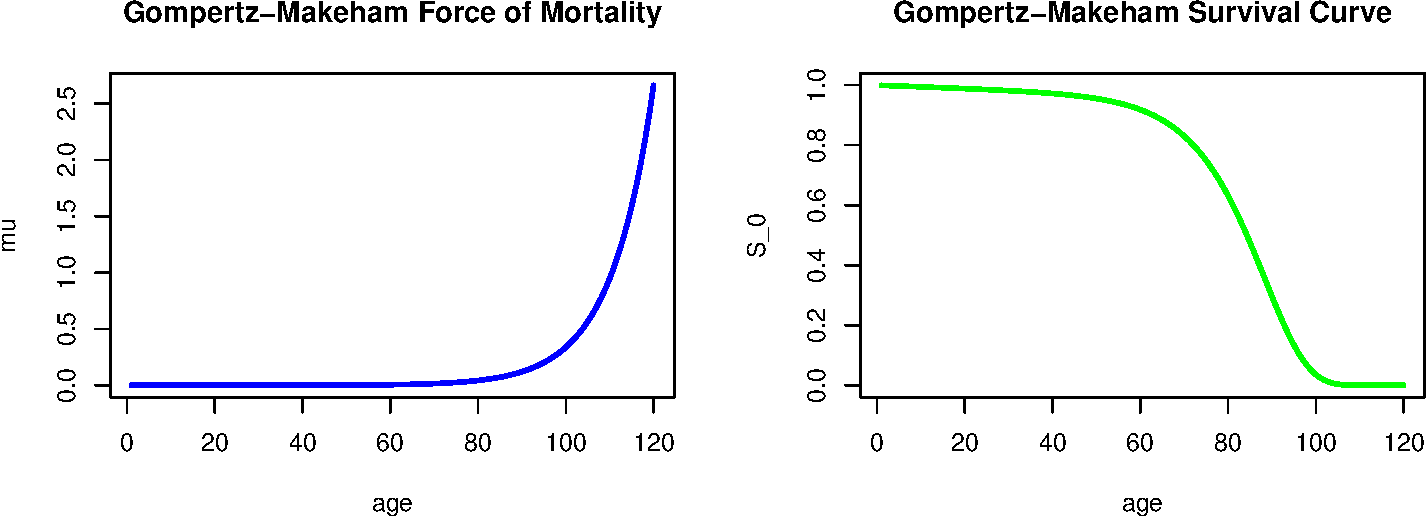
\includegraphics{LifeCon_files/figure-latex/SurvPlotFemUSDataFigsa-1} 

}

\caption{\textbf{Fitted Force of Mortality and Survival Curve}}\label{fig:SurvPlotFemUSDataFigsa}
\end{figure}

\hypertarget{S:LifeTab}{%
\section{Life Tables and their Functions}\label{S:LifeTab}}

As we illustrated in the previous section, the Gompertz-Makeham model is able to describe basic mortality patterns quite well -- and particularly match life expectancies across ages. However, the resulting force of mortality that is described by three parameters is highly regular. In particular, the likelihood of dying is monotonically increasing over the entire age domain. While this is true across many ages, real-world human mortality often shows a few deviations from these regular patterns. For instance, we often observe a so-called ``young adult mortality hump'' arising from risky behavior, involvement in wars, etc.

While there exist mortality laws that can account for this and other features, resulting functions quickly become complex and exhibit a low degree of tractability. Hence, a typical approach is to directly specify the survival function \(S_0(\cdot)\) of the lifetime random variable of a newborn within the ``age-only'' model and use it for actuarial calculations. Such an approach is often characterized as \emph{non-parametric} since the survival function is not given as a function of a few given parameters. We will discuss more advanced approaches to estimating non-parametric survival functions from mortality data in Section \ref{S:NonParamSurv}.

A rather simple approach in this direction is to construct so-called \emph{life tables}. As we discuss in the first part of this chapter, a life-table is simply an annually-discretized version of the survival function \(S_0(\cdot)\). A substantial advantage is that it is easy to generate such life tables from data in the context of population count data that we encountered in Section \ref{S:HMDData}, as we will see and do in the second section \ref{S:LifeTabEst}. The following sections \ref{S:LifeTabFrac} and \ref{S:LifeTabRec} the discuss some in more detail the theoretical underpinnings of life tables based on the so-called \emph{curtate} lifetime and how to drive quantities for \emph{fractional ages} based on the annually-discretized representation. Finally, the concluding sections \ref{S:LifeTabSelect} and \ref{S:LifeTabMImpr} discuss more advanced life tables that include underwriting (selection) effects and mortality improvements, respectively.

\hypertarget{S:LifeTabBasics}{%
\subsection{Life Table Basics}\label{S:LifeTabBasics}}

Consider a (large) population of \(l_0\) homogeneous newborns. Then, if survival in the population follows (exactly) the survival function \(S_0(\cdot)\), at age \(x\) there are
\[
l_0 \times S_0(x) = l_0 \times {_xp_0} = l_0 \times P(T_0 \geq x) = l_x
\]
individuals left. Of course, this immediately implies \({_xp_0} = \frac{l_x}{l_0}\) and, similarly, we can derive \(k\)-year the survival probability for an \(x\)-year old as:
\[
{_kp_x} = \frac{S_0(x+k)}{S_0(x)} = \frac{l_0 \times S_0(x+k)}{l_0 \times S_0(x)} = \frac{l_{x+k}}{l_x},\,x,k=0,1,2,...
\]
In particular, the set of \(l_x,\,x=0,1,2,...,\) lets us compute relevant probabilities for integer choices, which is not surprising because they are effectively providing an annually-discredited version of the survival function \(S_0(\cdot)\) in the age-only model. Evidently the so-called \emph{radix} \(l_0\) is immaterial, though it is typically chosen as a large number in line with the population interpretation, so that it is not necessary to display digits. A \emph{life table} provides exactly the set of \(l_x,\,x=0,1,2,...,\) typically compiled in a tabular manner starting at some initial age (maybe zero for a population table) up to some \emph{termimal age} \(\omega\) after which all individuals are assumed die, i.e., \(l_{\omega + 1} = 0.\)

From the above equation, we immediately obtain:
\[
{_kq_x} = 1 - {_kp_x} = \frac{l_x - l_{x+k}}{l_x} = \frac{_kd_x}{l_x},\,x,k=0,1,2,...
\]
where \(_kd_x\) denotes the \emph{deaths} between ages \(x\) and \(x+k\). In particular, we have:
\[
q_x = 1 - p_x = \frac{d_x}{l_x} \Leftrightarrow l_x - l_x\times p_x = d_x \Leftrightarrow l_{x+1} = l_x\times p_x = l_x - d_x,\,x=0,1,2,...
\]

This suggests one way of creating a life table: We could observe a (large) \emph{cohort} of \(l_0\) individuals initially, count the annual deaths \(d_0,\) \(d_1,\) etc., and tabulate the resulting survivors. The result would be a so-called \emph{cohort life table} as it reflects survivorship of the observed cohort over time. However, this approach is rather unpractical: we would have to wait until the last person in the cohort has deceased, and by then compiling a life table for an extinct cohort is likely of limited use.

The more common approach is to compile a so-called \emph{period life table}. Here instead of following a particular cohort, we consider a given population over a certain period, e.g.~a calendar year. We then use observed population mortality rates \(q_x\) in the time period to determine \(l_x\) for all ages according to relationship above. We explore this idea using the population mortality data we introduced in Section \ref{S:HMDData}.

\hypertarget{S:LifeTabEst}{%
\subsection{Life Table based on U.S. Population Data}\label{S:LifeTabEst}}

In section \ref{S:HMDData} we considered exposures and deaths of the U.S. population over time, and in particular in Figure \ref{fig:AllDRChapHMDUSFigsa} we plotted mortality rates---defined as the fraction of deaths and exposures---referencing the similarity to the Gompertz-Makeham law from Figure \ref{fig:SurvPlotFemUSDataFigsa}. It may be tempting to think about this mortality rates as \(q_x\) and use it to compile a life table. However, while the two quantities are related, there is a subtle difference: the mortality probability \(q_x = d_x/l_x\) considers deaths during age \(x\) relative to the population of \(x\) year olds.

In contrast, the \emph{central death rate} is defined as the number of deaths each year that have characteristics \(\bf{x}\) at the moment of death in the relevant observation period, divided by the exposures with the same characteristics \(\bf{x}\) over the same period, and is denoted as \(m_\bf{x}\)---where as usual we write \(m_{x}\) in the age-only model. Hence, in particular the denominator corresponds to the average size of the population at risk, not the population at risk at the outset.

To connect \(q_x\) and \(m_x\), we need to make an assumption about the exposure. One straightforward approach is to assume that the exposures correspond to the arithmetic average of the population size at age \(x\) and the population size at age \(x+1\), though different approaches are possible as we will see in Section \ref{S:LifeTabFrac}:
\[
m_x \approx \frac{d_x}{0.5\,l_x+ 0.5\,l_{x+1}} = \frac{q_x}{1-0.5\,q_x} \Longrightarrow q_x = \frac{2\,m_x}{2+m_x}.
\]

Let us use this relationship to construct a mortality life table using the 2010-2014 U.S.Females and Males data:

\begin{Shaded}
\begin{Highlighting}[]
\NormalTok{us_mx <-}\StringTok{ }\NormalTok{us_deaths }
\NormalTok{us_mx[,}\DecValTok{4}\OperatorTok{:}\DecValTok{6}\NormalTok{] <-}\StringTok{ }\NormalTok{us_deaths[,}\DecValTok{4}\OperatorTok{:}\DecValTok{6}\NormalTok{] }\OperatorTok{/}\StringTok{ }\NormalTok{us_exp[,}\DecValTok{4}\OperatorTok{:}\DecValTok{6}\NormalTok{]}
\NormalTok{us_mx_fem_}\DecValTok{2014}\NormalTok{ <-}\StringTok{ }\NormalTok{us_mx[us_mx}\OperatorTok{$}\NormalTok{Year_start }\OperatorTok{==}\StringTok{ }\DecValTok{2010}\NormalTok{,}\OperatorTok{-}\KeywordTok{c}\NormalTok{(}\DecValTok{2}\NormalTok{,}\DecValTok{5}\NormalTok{,}\DecValTok{6}\NormalTok{)]}
\KeywordTok{colnames}\NormalTok{(us_mx_fem_}\DecValTok{2014}\NormalTok{)[}\KeywordTok{colnames}\NormalTok{(us_mx_fem_}\DecValTok{2014}\NormalTok{)}\OperatorTok{==}\StringTok{"Female"}\NormalTok{] <-}\StringTok{ "mx US Females"}
\NormalTok{us_mx_fem_}\DecValTok{2014}\OperatorTok{$}\NormalTok{qx <-}\StringTok{ }\DecValTok{2} \OperatorTok{*}\StringTok{ }\NormalTok{us_mx_fem_}\DecValTok{2014}\OperatorTok{$}\NormalTok{mx }\OperatorTok{/}\StringTok{ }\NormalTok{(}\DecValTok{2} \OperatorTok{+}\StringTok{ }\NormalTok{us_mx_fem_}\DecValTok{2014}\OperatorTok{$}\NormalTok{mx)}
\KeywordTok{colnames}\NormalTok{(us_mx_fem_}\DecValTok{2014}\NormalTok{)[}\KeywordTok{colnames}\NormalTok{(us_mx_fem_}\DecValTok{2014}\NormalTok{)}\OperatorTok{==}\StringTok{"qx"}\NormalTok{] <-}\StringTok{ "qx US Females"}
\NormalTok{tmp_head_us_mx_fem_}\DecValTok{2014}\NormalTok{ <-}\StringTok{ }\KeywordTok{head}\NormalTok{(us_mx_fem_}\DecValTok{2014}\NormalTok{); }\KeywordTok{rownames}\NormalTok{(tmp_head_us_mx_fem_}\DecValTok{2014}\NormalTok{) <-}\StringTok{ }\OtherTok{NULL}
\KeywordTok{kable}\NormalTok{(}\KeywordTok{head}\NormalTok{(tmp_head_us_mx_fem_}\DecValTok{2014}\NormalTok{), }\DataTypeTok{align =} \StringTok{"ccr"}\NormalTok{)}
\end{Highlighting}
\end{Shaded}

\begin{tabular}{c|c|r|c}
\hline
Year\_start & Age & mx US Females & qx US Females\\
\hline
2010 & 0 & 0.005461737 & 0.005446862\\
\hline
2010 & 1 & 0.000379927 & 0.000379855\\
\hline
2010 & 2 & 0.000224890 & 0.000224865\\
\hline
2010 & 3 & 0.000169394 & 0.000169380\\
\hline
2010 & 4 & 0.000138322 & 0.000138313\\
\hline
2010 & 5 & 0.000119244 & 0.000119237\\
\hline
\end{tabular}

\begin{Shaded}
\begin{Highlighting}[]
\NormalTok{us_mx_mal_}\DecValTok{2014}\NormalTok{ <-}\StringTok{ }\NormalTok{us_mx[us_mx}\OperatorTok{$}\NormalTok{Year_start }\OperatorTok{==}\StringTok{ }\DecValTok{2010}\NormalTok{,}\OperatorTok{-}\KeywordTok{c}\NormalTok{(}\DecValTok{2}\NormalTok{,}\DecValTok{4}\NormalTok{,}\DecValTok{6}\NormalTok{)]}
\KeywordTok{colnames}\NormalTok{(us_mx_mal_}\DecValTok{2014}\NormalTok{)[}\KeywordTok{colnames}\NormalTok{(us_mx_mal_}\DecValTok{2014}\NormalTok{)}\OperatorTok{==}\StringTok{"Male"}\NormalTok{] <-}\StringTok{ "mx US Males"}
\NormalTok{us_mx_mal_}\DecValTok{2014}\OperatorTok{$}\NormalTok{qx <-}\StringTok{ }\DecValTok{2} \OperatorTok{*}\StringTok{ }\NormalTok{us_mx_mal_}\DecValTok{2014}\OperatorTok{$}\NormalTok{mx }\OperatorTok{/}\StringTok{ }\NormalTok{(}\DecValTok{2} \OperatorTok{+}\StringTok{ }\NormalTok{us_mx_mal_}\DecValTok{2014}\OperatorTok{$}\NormalTok{mx)}
\KeywordTok{colnames}\NormalTok{(us_mx_mal_}\DecValTok{2014}\NormalTok{)[}\KeywordTok{colnames}\NormalTok{(us_mx_mal_}\DecValTok{2014}\NormalTok{)}\OperatorTok{==}\StringTok{"qx"}\NormalTok{] <-}\StringTok{ "qx US Males"}
\NormalTok{tmp_head_us_mx_mal_}\DecValTok{2014}\NormalTok{ <-}\StringTok{ }\KeywordTok{head}\NormalTok{(us_mx_mal_}\DecValTok{2014}\NormalTok{); }\KeywordTok{rownames}\NormalTok{(tmp_head_us_mx_mal_}\DecValTok{2014}\NormalTok{) <-}\StringTok{ }\OtherTok{NULL}
\KeywordTok{kable}\NormalTok{(}\KeywordTok{head}\NormalTok{(tmp_head_us_mx_mal_}\DecValTok{2014}\NormalTok{), }\DataTypeTok{align =} \StringTok{"ccr"}\NormalTok{)}
\end{Highlighting}
\end{Shaded}

\begin{tabular}{c|c|r|c}
\hline
Year\_start & Age & mx US Males & qx US Males\\
\hline
2010 & 0 & 0.006554279 & 0.006532870\\
\hline
2010 & 1 & 0.000441664 & 0.000441567\\
\hline
2010 & 2 & 0.000298869 & 0.000298824\\
\hline
2010 & 3 & 0.000225097 & 0.000225072\\
\hline
2010 & 4 & 0.000184733 & 0.000184715\\
\hline
2010 & 5 & 0.000145992 & 0.000145981\\
\hline
\end{tabular}

The death probability curves for the U.S. Females and Males data are depicted in both original and logarithmic scales, and displayed as Figure \ref{fig:QxUSDataFigsa}.

R Code For Figure

\hypertarget{toggleCode.QxUSFemDataFigs}{}
\begin{Shaded}
\begin{Highlighting}[]
\KeywordTok{par}\NormalTok{(}\DataTypeTok{mfrow=}\KeywordTok{c}\NormalTok{(}\DecValTok{2}\NormalTok{,}\DecValTok{2}\NormalTok{))}
\KeywordTok{plot}\NormalTok{(us_mx_fem_}\DecValTok{2014}\OperatorTok{$}\NormalTok{qx,}\DataTypeTok{type =} \StringTok{"l"}\NormalTok{, }\DataTypeTok{lwd =} \DecValTok{5}\NormalTok{, }\DataTypeTok{col =} \StringTok{"blue"}\NormalTok{, }\DataTypeTok{main=}\StringTok{"Original scale Female"}\NormalTok{, }\DataTypeTok{xlab =} \StringTok{"age"}\NormalTok{, }\DataTypeTok{ylab =} \StringTok{"q_x"}\NormalTok{,}\DataTypeTok{ylim =} \KeywordTok{c}\NormalTok{(}\DecValTok{0}\NormalTok{,}\FloatTok{1.0}\NormalTok{))}
\KeywordTok{lines}\NormalTok{(us_mx_fem_}\DecValTok{2014}\OperatorTok{$}\NormalTok{mx,}\DataTypeTok{col=}\StringTok{"red"}\NormalTok{)}
\KeywordTok{plot}\NormalTok{(}\KeywordTok{log}\NormalTok{(us_mx_fem_}\DecValTok{2014}\OperatorTok{$}\NormalTok{qx, }\DataTypeTok{base =} \DecValTok{10}\NormalTok{),}\DataTypeTok{type =} \StringTok{"l"}\NormalTok{, }\DataTypeTok{lwd =} \DecValTok{5}\NormalTok{, }\DataTypeTok{col =} \StringTok{"blue"}\NormalTok{, }\DataTypeTok{main=}\StringTok{"Log scale Female"}\NormalTok{, }\DataTypeTok{xlab =} \StringTok{"age"}\NormalTok{, }\DataTypeTok{ylab =} \StringTok{"q_x"}\NormalTok{)}
\KeywordTok{plot}\NormalTok{(us_mx_mal_}\DecValTok{2014}\OperatorTok{$}\NormalTok{qx,}\DataTypeTok{type =} \StringTok{"l"}\NormalTok{, }\DataTypeTok{lwd =} \DecValTok{5}\NormalTok{, }\DataTypeTok{col =} \StringTok{"blue"}\NormalTok{, }\DataTypeTok{main=}\StringTok{"Original scale Male"}\NormalTok{, }\DataTypeTok{xlab =} \StringTok{"age"}\NormalTok{, }\DataTypeTok{ylab =} \StringTok{"q_x"}\NormalTok{,}\DataTypeTok{ylim =} \KeywordTok{c}\NormalTok{(}\DecValTok{0}\NormalTok{,}\FloatTok{1.0}\NormalTok{))}
\KeywordTok{lines}\NormalTok{(us_mx_mal_}\DecValTok{2014}\OperatorTok{$}\NormalTok{mx,}\DataTypeTok{col=}\StringTok{"red"}\NormalTok{)}
\KeywordTok{plot}\NormalTok{(}\KeywordTok{log}\NormalTok{(us_mx_mal_}\DecValTok{2014}\OperatorTok{$}\NormalTok{qx, }\DataTypeTok{base =} \DecValTok{10}\NormalTok{),}\DataTypeTok{type =} \StringTok{"l"}\NormalTok{, }\DataTypeTok{lwd =} \DecValTok{5}\NormalTok{, }\DataTypeTok{col =} \StringTok{"blue"}\NormalTok{, }\DataTypeTok{main=}\StringTok{"Log scale Male"}\NormalTok{, }\DataTypeTok{xlab =} \StringTok{"age"}\NormalTok{, }\DataTypeTok{ylab =} \StringTok{"q_x"}\NormalTok{)}
\end{Highlighting}
\end{Shaded}



\begin{figure}

{\centering 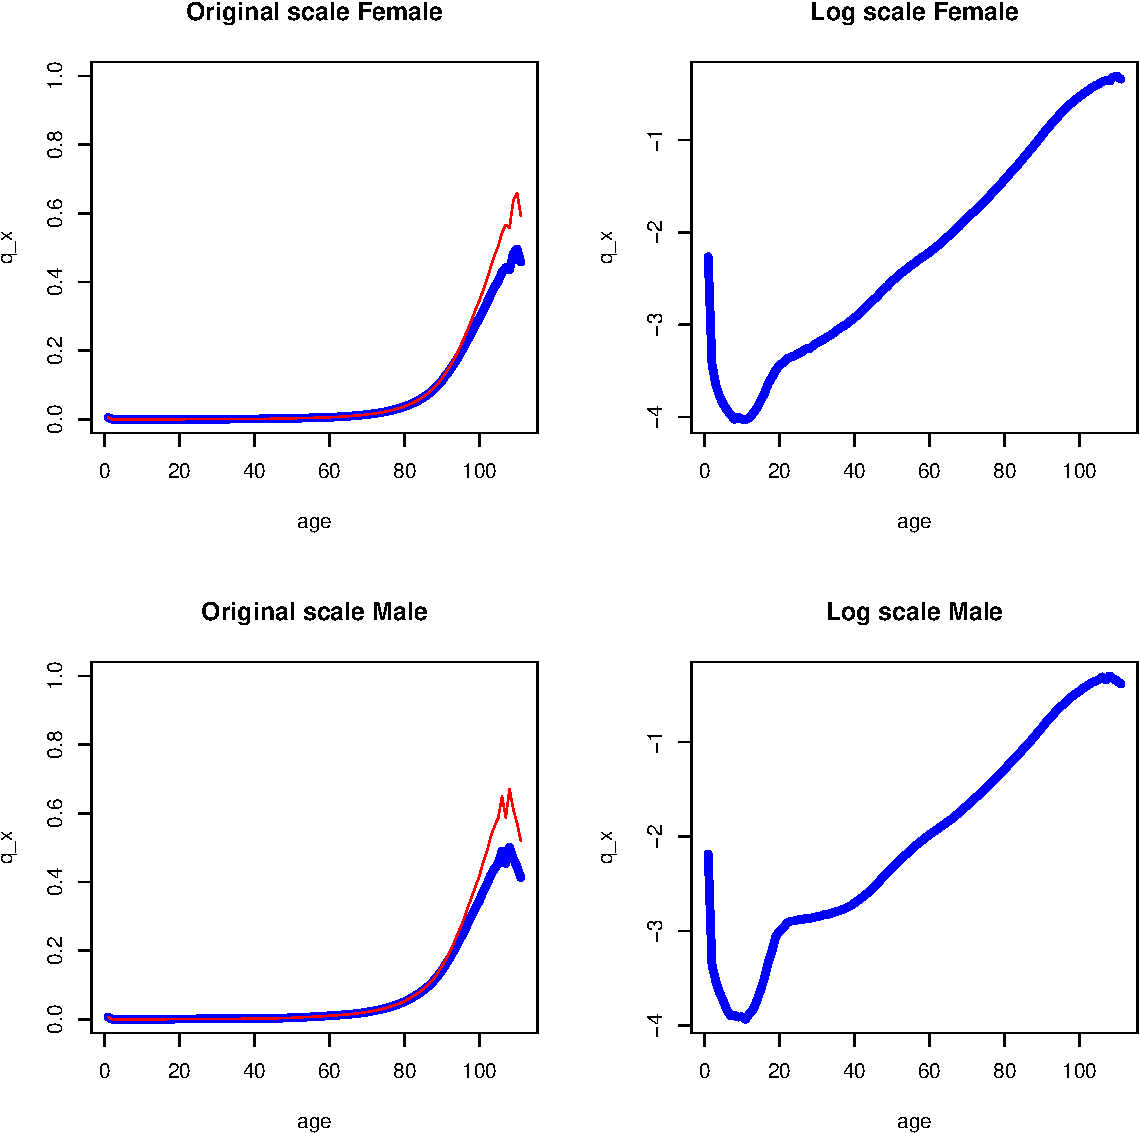
\includegraphics{LifeCon_files/figure-latex/QxUSFemDataFigsa-1} 

}

\caption{\textbf{One year death probability curve (in blue) and central death rate (in red) for the 2010-2014 U.S. data across all ages}}\label{fig:QxUSFemDataFigsa}
\end{figure}

As we can see, \(q_x\) and \(m_x\) are similar with the exception of the later years. As expected, the log scale plots are more informative in the sense that the log scale reveals the marginal changes over various ages, and we now combined the two log scaled curves into Figure \ref{fig:QxUSFemMalDataFigsa}.

R Code For Figure

\hypertarget{toggleCode.QxUSFemMalDataFigs}{}
\begin{Shaded}
\begin{Highlighting}[]
\KeywordTok{par}\NormalTok{(}\DataTypeTok{mfrow=}\KeywordTok{c}\NormalTok{(}\DecValTok{1}\NormalTok{,}\DecValTok{1}\NormalTok{))}
\KeywordTok{plot}\NormalTok{(}\KeywordTok{log}\NormalTok{(us_mx_fem_}\DecValTok{2014}\OperatorTok{$}\NormalTok{qx, }\DataTypeTok{base =} \DecValTok{10}\NormalTok{), }\DataTypeTok{type =} \StringTok{"l"}\NormalTok{, }\DataTypeTok{lwd =} \DecValTok{5}\NormalTok{, }\DataTypeTok{col =} \StringTok{"blue"}\NormalTok{, }\DataTypeTok{main=}\StringTok{"Log scale"}\NormalTok{, }\DataTypeTok{xlab =} \StringTok{"age"}\NormalTok{, }\DataTypeTok{ylab =} \StringTok{"q_x"}\NormalTok{)}
\KeywordTok{lines}\NormalTok{(}\KeywordTok{log}\NormalTok{(us_mx_mal_}\DecValTok{2014}\OperatorTok{$}\NormalTok{qx, }\DataTypeTok{base =} \DecValTok{10}\NormalTok{), }\DataTypeTok{lwd =} \DecValTok{5}\NormalTok{, }\DataTypeTok{col =} \StringTok{"red"}\NormalTok{)}
\end{Highlighting}
\end{Shaded}



\begin{figure}

{\centering 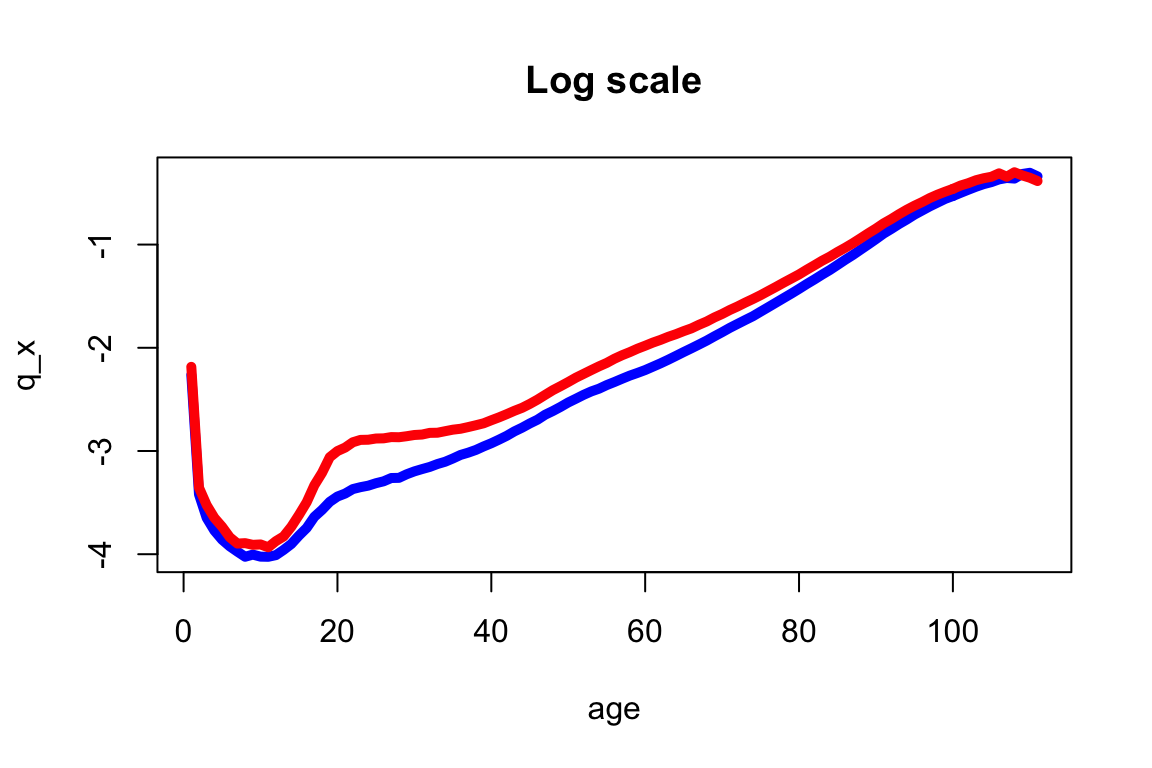
\includegraphics{LifeCon_files/figure-latex/QxUSFemMalDataFigsa-1} 

}

\caption{\textbf{One year death probability curve for the 2010-2014 U.S. Females (in blue) and Males (in red) data across all ages}}\label{fig:QxUSFemMalDataFigsa}
\end{figure}

Figure \ref{fig:QxUSFemMalDataFigsa} shows the usual higher mortality rates for males than for females, but also extremely pronounced differences at ages 16 to 40 that could be explained by social factors that are specific to U.S. Males at post adolescence ages. As indicated before, these intricacies are not accounted for by the Gompertz-Makeham and other simple parametric models. Moreover, significant differences at ages 50 to 70 are also observed, and are due to health related factors that males around the world tend to be exposed earlier than females.

We are now able to construct a \emph{period life table} based on the U.S. mortality data. Using the relationships from before:
\[
l_{x+1}=l_x\cdot p_x=l_x\big(1-q_x\big)\quad\text{for all integers}\quad x.
\]
and fixing \(l_0 = 1,000,000\), we generate \(l_x\), \(x=0,1,2,...\), for the male and female life table:

\begin{Shaded}
\begin{Highlighting}[]
\NormalTok{lf <-}\StringTok{ }\KeywordTok{rep}\NormalTok{(}\DecValTok{0}\NormalTok{,}\KeywordTok{length}\NormalTok{(us_mx_fem_}\DecValTok{2014}\OperatorTok{$}\NormalTok{mx))}
\NormalTok{lf[}\DecValTok{1}\NormalTok{] <-}\StringTok{ }\DecValTok{1000000}
\ControlFlowTok{for}\NormalTok{ (i }\ControlFlowTok{in} \DecValTok{2}\OperatorTok{:}\DecValTok{111}\NormalTok{)\{}
\NormalTok{  lf[i] =}\StringTok{ }\NormalTok{lf[i}\DecValTok{-1}\NormalTok{] }\OperatorTok{*}\StringTok{ }\NormalTok{(}\DecValTok{1}\OperatorTok{-}\NormalTok{us_mx_fem_}\DecValTok{2014}\NormalTok{[i}\DecValTok{-1}\NormalTok{,}\DecValTok{4}\NormalTok{]) }
\NormalTok{\}}
\NormalTok{us_mx_fem_}\DecValTok{2014}\OperatorTok{$}\NormalTok{lf <-}\StringTok{ }\NormalTok{lf}

\NormalTok{lm <-}\StringTok{ }\KeywordTok{rep}\NormalTok{(}\DecValTok{0}\NormalTok{,}\KeywordTok{length}\NormalTok{(us_mx_mal_}\DecValTok{2014}\OperatorTok{$}\NormalTok{mx))}
\NormalTok{lm[}\DecValTok{1}\NormalTok{] <-}\StringTok{ }\DecValTok{1000000}
\ControlFlowTok{for}\NormalTok{ (i }\ControlFlowTok{in} \DecValTok{2}\OperatorTok{:}\DecValTok{111}\NormalTok{)\{}
\NormalTok{  lm[i] =}\StringTok{ }\NormalTok{lm[i}\DecValTok{-1}\NormalTok{] }\OperatorTok{*}\StringTok{ }\NormalTok{(}\DecValTok{1}\OperatorTok{-}\NormalTok{us_mx_mal_}\DecValTok{2014}\NormalTok{[i}\DecValTok{-1}\NormalTok{,}\DecValTok{4}\NormalTok{])}
\NormalTok{\}}
\NormalTok{us_mx_mal_}\DecValTok{2014}\OperatorTok{$}\NormalTok{lm <-}\StringTok{ }\NormalTok{lm}
\end{Highlighting}
\end{Shaded}

Resulting in, for females:

\begin{Shaded}
\begin{Highlighting}[]
\KeywordTok{library}\NormalTok{(DT)}
\NormalTok{tmp_life_table_us_mx_fem_}\DecValTok{2014}\NormalTok{ <-}\StringTok{ }\KeywordTok{round}\NormalTok{(us_mx_fem_}\DecValTok{2014}\NormalTok{, }\DataTypeTok{digits =} \DecValTok{9}\NormalTok{); }
\KeywordTok{colnames}\NormalTok{(tmp_life_table_us_mx_fem_}\DecValTok{2014}\NormalTok{)[}\DecValTok{5}\NormalTok{]<-}\StringTok{ "lx US Females"}

\KeywordTok{rownames}\NormalTok{(tmp_life_table_us_mx_fem_}\DecValTok{2014}\NormalTok{) <-}\StringTok{ }\OtherTok{NULL}
\CommentTok{#kable(tmp_life_table_us_mx_fem_2014, digits = 9, format.args = list(big.mark = ","), align = "ccrrr")}
\NormalTok{DT}\OperatorTok{::}\KeywordTok{datatable}\NormalTok{(tmp_life_table_us_mx_fem_}\DecValTok{2014}\NormalTok{)}
\end{Highlighting}
\end{Shaded}

\begin{center}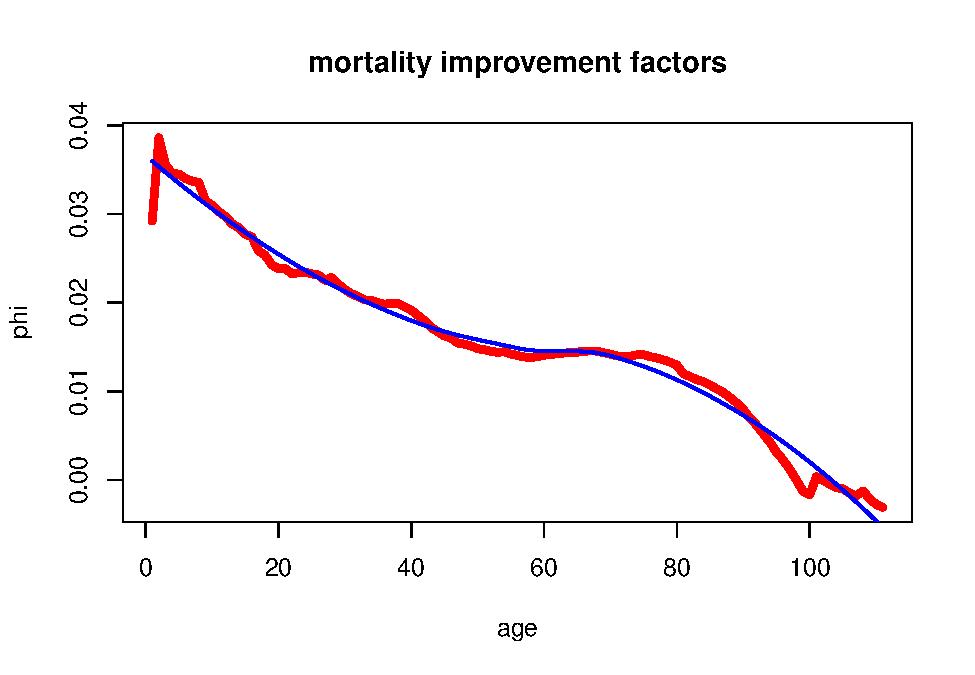
\includegraphics{LifeCon_files/figure-latex/unnamed-chunk-27-1} \end{center}

And for males:

\begin{Shaded}
\begin{Highlighting}[]
\NormalTok{tmp_life_table_us_mx_mal_}\DecValTok{2014}\NormalTok{ <-}\KeywordTok{round}\NormalTok{(us_mx_mal_}\DecValTok{2014}\NormalTok{, }\DataTypeTok{digits =} \DecValTok{9}\NormalTok{); }
\KeywordTok{colnames}\NormalTok{(tmp_life_table_us_mx_mal_}\DecValTok{2014}\NormalTok{)[}\DecValTok{5}\NormalTok{]<-}\StringTok{ "lx US Males"}
\KeywordTok{rownames}\NormalTok{(tmp_life_table_us_mx_mal_}\DecValTok{2014}\NormalTok{) <-}\StringTok{ }\OtherTok{NULL}
\CommentTok{#kable(tmp_life_table_us_mx_mal_2014, digits = 9, format.args = list(big.mark = ","), align = "ccrrr") }
\NormalTok{DT}\OperatorTok{::}\KeywordTok{datatable}\NormalTok{(tmp_life_table_us_mx_mal_}\DecValTok{2014}\NormalTok{) }
\end{Highlighting}
\end{Shaded}

\begin{center}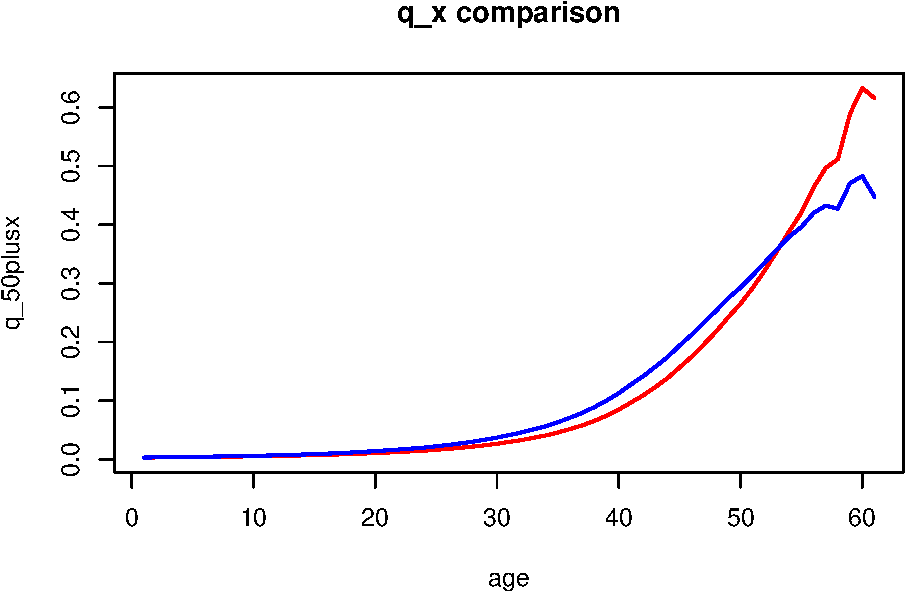
\includegraphics{LifeCon_files/figure-latex/unnamed-chunk-28-1} \end{center}

The \(l_x\) values are now plotted in Figure \ref{fig:LxMalFemDataFigsa} where once again the female subpopulation shows higher survivorship trend than the male subpopulation.

R Code For Figure

\hypertarget{toggleCode.QxUSFemMalDataFigs}{}
\begin{Shaded}
\begin{Highlighting}[]
\KeywordTok{plot}\NormalTok{(lf, }\DataTypeTok{type =} \StringTok{"l"}\NormalTok{, }\DataTypeTok{lwd =} \DecValTok{5}\NormalTok{, }\DataTypeTok{col =} \StringTok{"yellow"}\NormalTok{, }\DataTypeTok{xlab =} \StringTok{"age"}\NormalTok{, }\DataTypeTok{ylab =} \StringTok{"l_x"}\NormalTok{,}\DataTypeTok{ylim =} \KeywordTok{c}\NormalTok{(}\DecValTok{0}\NormalTok{,}\DecValTok{1000000}\NormalTok{))}
\KeywordTok{lines}\NormalTok{(lm, }\DataTypeTok{type =} \StringTok{"l"}\NormalTok{, }\DataTypeTok{lwd =} \DecValTok{5}\NormalTok{, }\DataTypeTok{col =} \StringTok{"orange"}\NormalTok{, }\DataTypeTok{xlab =} \StringTok{"age"}\NormalTok{, }\DataTypeTok{ylab =} \StringTok{"l_x"}\NormalTok{,}\DataTypeTok{ylim =} \KeywordTok{c}\NormalTok{(}\DecValTok{0}\NormalTok{,}\DecValTok{1000000}\NormalTok{))}
\end{Highlighting}
\end{Shaded}



\begin{figure}

{\centering 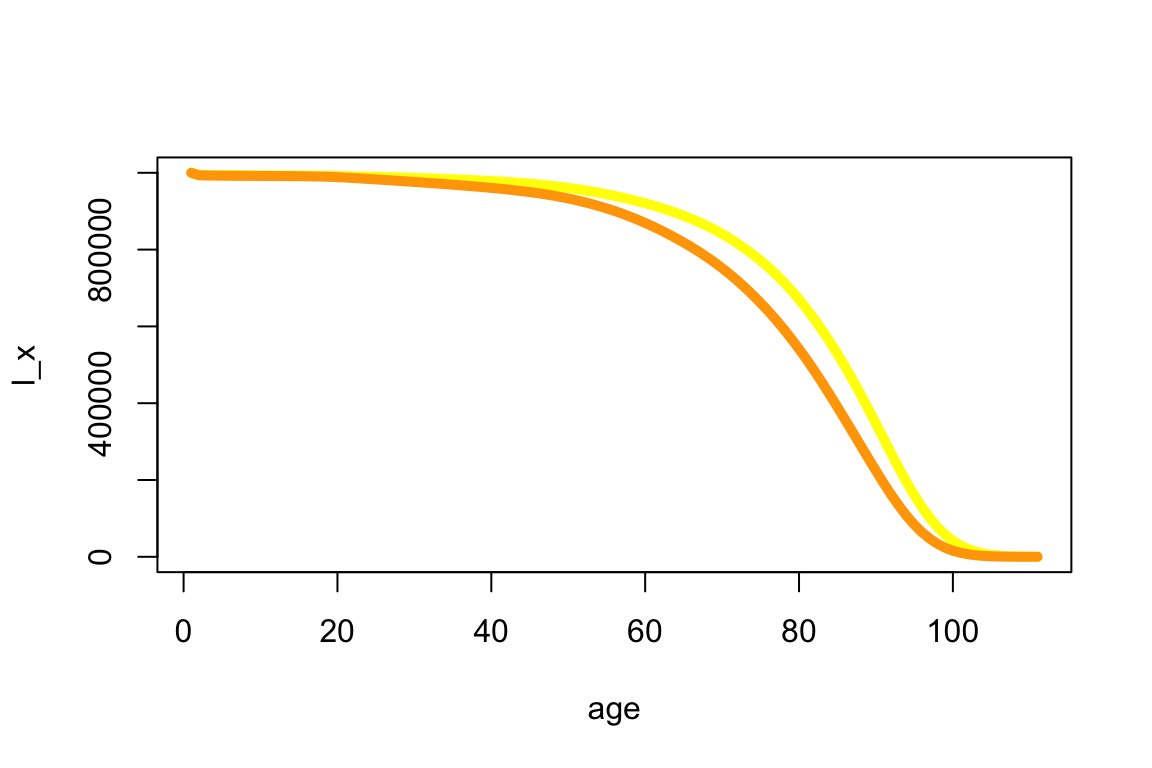
\includegraphics{LifeCon_files/figure-latex/LxMalFemDataFigsa-1} 

}

\caption{\textbf{Expected number at risk for the 2010-2014 U.S. Females (in yellow) and Males (in orange) data across all ages}}\label{fig:LxMalFemDataFigsa}
\end{figure}

There are more advanced approaches to fine-tune the life table, e.g.~by smoothing approaches to adjust small deviations in the observed mortality data. However, when relying on the sizable U.S. population, the resulting quantities are fairly smooth as illustrated by Figures \ref{fig:QxUSFemMalDataFigsa} and \ref{fig:LxMalFemDataFigsa}. Hence, we will rely on them without adjustments.

We can rely on the life table to determine various actuarial quantities, at integer ages and for integer durations. For instance, we can determine the survival probabilities \(_kp_{50}\) for a 50-year-old female for all choices of \(k=0,1,2,...\):

\begin{Shaded}
\begin{Highlighting}[]
\NormalTok{kP50 <-}\StringTok{ }\NormalTok{us_mx_fem_}\DecValTok{2014}\OperatorTok{$}\NormalTok{l[}\DecValTok{51}\OperatorTok{:}\DecValTok{111}\NormalTok{]}\OperatorTok{/}\NormalTok{us_mx_fem_}\DecValTok{2014}\OperatorTok{$}\NormalTok{l[}\DecValTok{51}\NormalTok{]}
\end{Highlighting}
\end{Shaded}

R Code For Figure

\hypertarget{toggleCode.kPxux2050-yearux20oldux20female}{}
\begin{Shaded}
\begin{Highlighting}[]
\KeywordTok{plot}\NormalTok{(kP50,}\DataTypeTok{xlab=}\StringTok{"age"}\NormalTok{, }\DataTypeTok{type =} \StringTok{"l"}\NormalTok{, }\DataTypeTok{lwd =} \DecValTok{5}\NormalTok{, }\DataTypeTok{col =} \StringTok{"red"}\NormalTok{)}
\end{Highlighting}
\end{Shaded}



\begin{figure}

{\centering 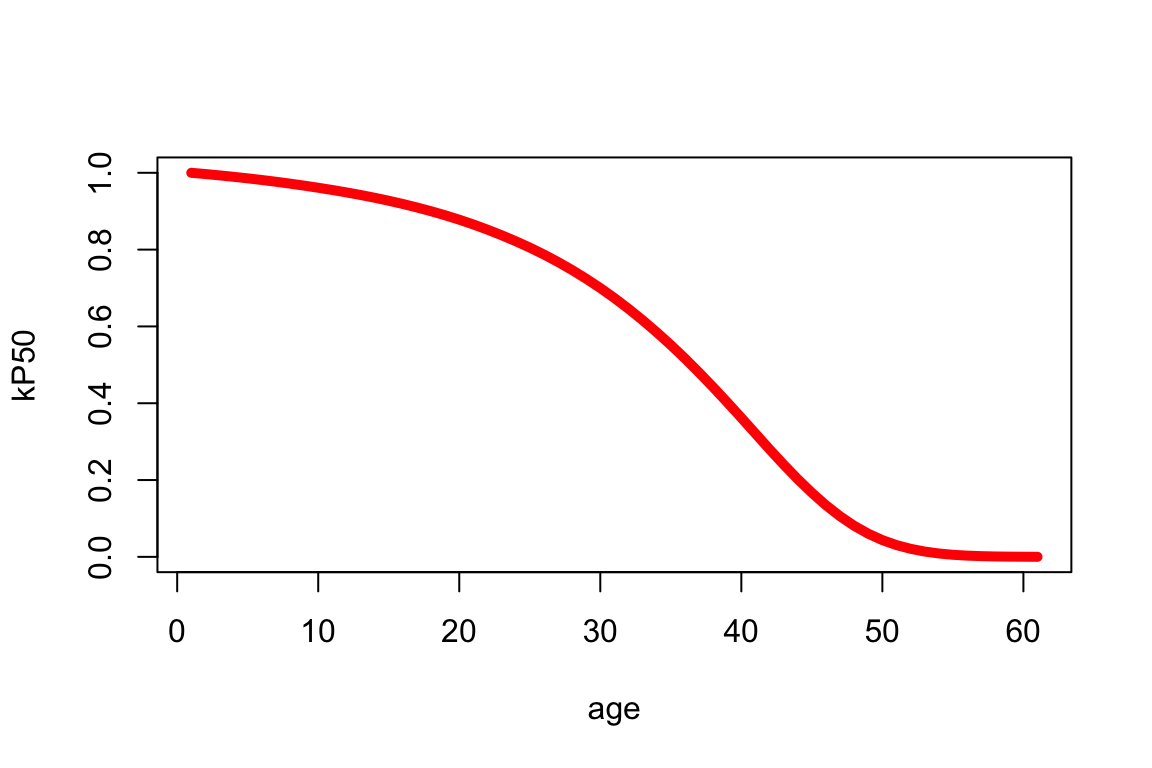
\includegraphics{LifeCon_files/figure-latex/kp50FemFiga-1} 

}

\caption{\textbf{kPx for a 50-year old female}}\label{fig:kp50FemFiga}
\end{figure}

Or we can determine \(_{10|20}q_{50}\), the probability that a 50-year old survives for 10 years and then dies within the next 20 years via \(\frac{l_{60}-l_{80}}{l_{50}}\):

\begin{Shaded}
\begin{Highlighting}[]
\NormalTok{(us_mx_fem_}\DecValTok{2014}\OperatorTok{$}\NormalTok{l[}\DecValTok{61}\NormalTok{] }\OperatorTok{-}\StringTok{ }\NormalTok{us_mx_fem_}\DecValTok{2014}\OperatorTok{$}\NormalTok{l[}\DecValTok{81}\NormalTok{])}\OperatorTok{/}\NormalTok{us_mx_fem_}\DecValTok{2014}\OperatorTok{$}\NormalTok{l[}\DecValTok{51}\NormalTok{]}
\end{Highlighting}
\end{Shaded}

\begin{verbatim}
[1] 0.281351377
\end{verbatim}

\hypertarget{S:LifeTabRec}{%
\subsection{Curtate Quantities and Recursive Relationships}\label{S:LifeTabRec}}

Rather than thinking about life tables as an annually-discretized version of the survival function of \(T_0\) within the age-only model, it is also possible to interpret a life table as providing probabilities of a discretized version of the lifetime random variable. This is referred to as the \emph{curtate future lifetime}.

Formally, the curtate future lifetime \(K_{\bf{x}}\) is given by the greatest integer of \(T_{\bf{x}}\): \(K_{\bf{x}} = \lfloor T_{\bf{x}} \rfloor\), i.e.\\
\begin{eqnarray*}
K_{\bf{x}} = 0 & \text{ if } & T_{\bf{x}} < 1\\
K_{\bf{x}} = 1 & \text{ if } & 1\leq  T_{\bf{x}} < 2\\
&...&\\
K_x = {\bf{x}} & \text{ if } & k \leq T_{\bf{x}} < k+1,\, k \in {\mathbb N}.
\end{eqnarray*}
Therefore, \(K_{\bf{x}}\) describes the number of whole future years lived by an individual with characteristics \({\bf{x}}\) prior to death. Therefore, the probability function of the (discrete) distribution of \(K_{\bf{x}}\) is:
\[
Pr(K_{\bf{x}} = k) = Pr(k \leq T_{\bf{x}} < k+1) = {_kp_{\bf{x}}} - {_{k+1}p_{\bf{x}}} = {_{k\mid 1}q_{\bf{x}}} = {_{k\mid}q_{\bf{x}}},\,k=0,1,...
\]

Just as for the lifetime, the expected value of \(K_x\) corresponds to a life expectancy, though this is a curtate version of life expectancy. It is denoted by \(e_{\bf{x}}\), and its calculation can be obtained by summing up the \({_kp_{\bf{x}}}\) in analogy to the derivation of (complete) life expectancy:
\[
e_{\bf{x}} = E[K_{\bf{x}}]= \sum_{k=1}^{\infty} {_kp_{\bf{x}}}.
\]

Derivation of Formula for Curtate Life Expectancy

\leavevmode\hypertarget{toggleTheory.DerivationCurtLifeExp}{}%
\begin{eqnarray*}
e_{\bf{x}} &=& E[K_{\bf{x}}] = \sum_{k=0}^{\infty} k \, Pr(K_{\bf{x}}=k) = \sum_{k=0}^{\infty} k\, ({_kp_{\bf{x}}} - {_{k+1}p_{\bf{x}}}) \\
&=& \sum_{k=0}^{\infty} k\, {_kp_{\bf{x}}}-\sum_{k=0}^{\infty} (k+1)\, {_{k+1}p_{\bf{x}}} + \sum_{k=0}^{\infty}  {_{k+1}p_{\bf{x}}}\\
&=&\sum_{k=1}^{\infty} {_kp_{\bf{x}}}.
\end{eqnarray*}

As before, in the age-only model we write \({\bf{x}}=x\), and in this case we can express the curtate expected lifetime of an \(x\)-year old by the corresponding value for an \(x+1\) year old:
\begin{eqnarray*}
e_x &=& \sum_{k=1}^{\infty} {_kp_x} = p_x \,\sum_{k=1}^{\infty} {_{k-1}p_{x+1}}
= p_x\,{_0p_{x+1}} + p_x\,\sum_{k=2}^{\infty} {_{k-1}p_{x+1}}  \\
&=& p_x + p_x \sum_{i=1}^{\infty} {_{i}p_{x+1}} = p_x + p_x \cdot e_{x+1}
\end{eqnarray*}
or
\[
e_{x} = p_x\left(1+e_{x+1}\right) 
\Leftrightarrow e_{x+1} = \frac{e_x - p_x}{p_x}.
\]
This \emph{recursive} formula states that the expected future lifetime for an \(x\)-year-old in whole years will be non-zero for the survivors until age \(x+1\) only, and for those it will be the expected future lifetime in whole years for an \(x+1\)-year-old individual plus the one year they already have survived.

Curtate life expectancies are straightforward to calculate from a life table. For instance, using our life table for females, we obtain for curtate life expectancy at birth is:

\begin{Shaded}
\begin{Highlighting}[]
\NormalTok{kP0f <-}\StringTok{ }\NormalTok{us_mx_fem_}\DecValTok{2014}\OperatorTok{$}\NormalTok{l}\OperatorTok{/}\NormalTok{us_mx_fem_}\DecValTok{2014}\OperatorTok{$}\NormalTok{l[}\DecValTok{1}\NormalTok{]}
\NormalTok{e_}\DecValTok{0}\NormalTok{ <-}\StringTok{ }\KeywordTok{sum}\NormalTok{(kP0f) }\OperatorTok{-}\StringTok{ }\DecValTok{1}
\NormalTok{e_}\DecValTok{0}
\end{Highlighting}
\end{Shaded}

\begin{verbatim}
[1] 80.7955575
\end{verbatim}

which is close to the Figure from the U.S. national statistics from Section \ref{S:DataLifeExp}, where the female life expectancy for 2017 is recorded as 81.1 years. We are also now in a position to elaborate on the caveat at the end of that section on the interpretation of this number: This is a so-called \emph{period life expectancy} as it was derived from a \emph{period life table}. So rather than reflecting the prospective life expectancy of a newborn today, it describes how long a hypothetical newborn that will have the mortality patterns observed in the population within this period will be expected to live. We will attempt to derive a more representative figure for a 50-year old alive today that will experience \emph{future} mortality rates in Section \ref{S:LifeTabMImpr}.

Indeed, an interesting and revealing exercise is to go through past years of data that we have available in our population count data from Section \ref{S:HMDData}, and derive life expectancies for past periods. We consider newborn and fifty-year-old females. We obtain this by essentially repeating the same exercise we carried out in the previous section to assemble the life table for every time period.

R Code For Figure

\hypertarget{toggleCode.Femaleux20lifeux20expectanciesux20acrossux20time}{}
\begin{Shaded}
\begin{Highlighting}[]
\NormalTok{e0 <-}\StringTok{ }\KeywordTok{rep}\NormalTok{(}\DecValTok{0}\NormalTok{,}\DecValTok{16}\NormalTok{)}
\NormalTok{e50 <-}\StringTok{ }\KeywordTok{rep}\NormalTok{(}\DecValTok{0}\NormalTok{,}\DecValTok{16}\NormalTok{)}

\NormalTok{i <-}\StringTok{ }\DecValTok{1}

\ControlFlowTok{for}\NormalTok{ (s }\ControlFlowTok{in} \KeywordTok{seq}\NormalTok{(}\DecValTok{1935}\NormalTok{,}\DecValTok{2010}\NormalTok{,}\DecValTok{5}\NormalTok{))\{}
  \CommentTok{#Get central death rates for each start year}
\NormalTok{  mx <-}\StringTok{ }\NormalTok{us_mx[us_mx}\OperatorTok{$}\NormalTok{Year_start }\OperatorTok{==}\StringTok{ }\NormalTok{s,}\DecValTok{4}\NormalTok{]}
\NormalTok{  S0 <-}\StringTok{ }\KeywordTok{rep}\NormalTok{(}\DecValTok{0}\NormalTok{,}\DecValTok{111}\NormalTok{)}
  
  \CommentTok{#Calculate the survival function}
\NormalTok{  S0[}\DecValTok{1}\NormalTok{] <-}\StringTok{ }\DecValTok{1}
  \ControlFlowTok{for}\NormalTok{ (j }\ControlFlowTok{in} \DecValTok{2}\OperatorTok{:}\DecValTok{111}\NormalTok{)\{}
\NormalTok{    S0[j] <-}\StringTok{ }\NormalTok{S0[j}\DecValTok{-1}\NormalTok{]}\OperatorTok{*}\NormalTok{(}\DecValTok{1} \OperatorTok{-}\StringTok{ }\NormalTok{(}\DecValTok{2}\OperatorTok{*}\NormalTok{mx[j}\DecValTok{-1}\NormalTok{])}\OperatorTok{/}\NormalTok{(}\DecValTok{2} \OperatorTok{+}\StringTok{ }\NormalTok{mx[j}\DecValTok{-1}\NormalTok{]))}
\NormalTok{  \}}

  \CommentTok{#And evaluate curtate life expectancies by summing over kPx's}
\NormalTok{  e0[i] <-}\StringTok{ }\KeywordTok{sum}\NormalTok{(S0) }\OperatorTok{-}\StringTok{ }\DecValTok{1}
\NormalTok{  e50[i] <-}\StringTok{ }\KeywordTok{sum}\NormalTok{(S0[}\DecValTok{51}\OperatorTok{:}\DecValTok{111}\NormalTok{]}\OperatorTok{/}\NormalTok{S0[}\DecValTok{51}\NormalTok{]) }\OperatorTok{-}\StringTok{ }\DecValTok{1}
\NormalTok{  i <-}\StringTok{ }\NormalTok{i}\OperatorTok{+}\DecValTok{1}
\NormalTok{\}}

\KeywordTok{par}\NormalTok{(}\DataTypeTok{mfrow=}\KeywordTok{c}\NormalTok{(}\DecValTok{1}\NormalTok{,}\DecValTok{2}\NormalTok{))}
\KeywordTok{plot}\NormalTok{(}\KeywordTok{seq}\NormalTok{(}\DecValTok{1935}\NormalTok{,}\DecValTok{2010}\NormalTok{,}\DecValTok{5}\NormalTok{),e0, }\DataTypeTok{type =} \StringTok{"l"}\NormalTok{, }\DataTypeTok{lwd =} \DecValTok{5}\NormalTok{, }\DataTypeTok{col =} \StringTok{"blue"}\NormalTok{, }\DataTypeTok{main=}\StringTok{"life expectancies at birth, across years"}\NormalTok{, }\DataTypeTok{xlab =} \StringTok{"year"}\NormalTok{, }\DataTypeTok{ylab =} \StringTok{"life expectancy"}\NormalTok{)}
\KeywordTok{plot}\NormalTok{(}\KeywordTok{seq}\NormalTok{(}\DecValTok{1935}\NormalTok{,}\DecValTok{2010}\NormalTok{,}\DecValTok{5}\NormalTok{),e50, }\DataTypeTok{type =} \StringTok{"l"}\NormalTok{, }\DataTypeTok{lwd =} \DecValTok{5}\NormalTok{, }\DataTypeTok{col =} \StringTok{"red"}\NormalTok{, }\DataTypeTok{main=}\StringTok{"life expectancies at 50, across years"}\NormalTok{, }\DataTypeTok{xlab =} \StringTok{"year"}\NormalTok{, }\DataTypeTok{ylab =} \StringTok{"life expectancy"}\NormalTok{)}
\end{Highlighting}
\end{Shaded}



\begin{figure}

{\centering 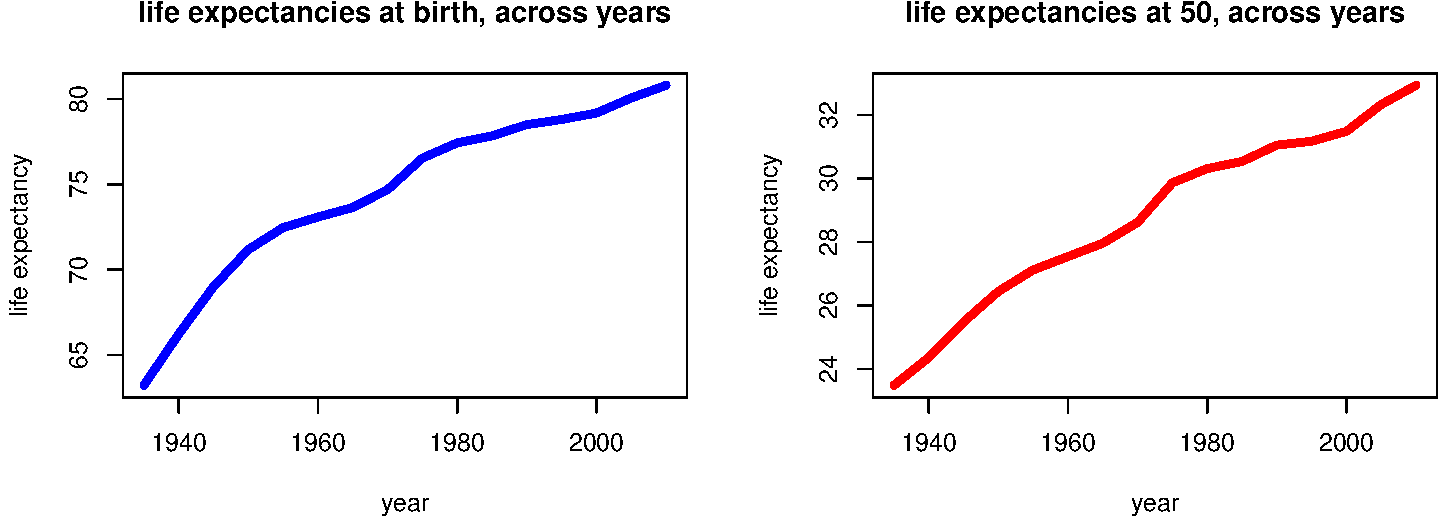
\includegraphics{LifeCon_files/figure-latex/exFemFiga-1} 

}

\caption{\textbf{Female life expectancies across time for U.S. females}}\label{fig:exFemFiga}
\end{figure}

We notice that period life expectancies have consistently increased, and indeed the increase seems close to linear. This is a familiar observation from demography, where it is pointed out that various limits on life expectancy that were previously assumed have been broken.

\hypertarget{S:LifeTabFrac}{%
\subsection{Fractional year assumptions}\label{S:LifeTabFrac}}

Let us consider the \emph{complete} life expectancy in the age-only model for an \(x\)-year old life or, more precisely, the \emph{recursive} relationship:
\begin{eqnarray*}
\stackrel{\circ}{e}_{x} &=& \int_0^{\infty} {_tp_x}\,dt = \int_0^{1} {_tp_x}\,dt +\int_1^{\infty} {_tp_x}\,dt 
= \int_0^{1} {_tp_x}\,dt +p_x\,\int_1^{\infty} {_{t-1}p_{x+1}}\,dt \\
&=&  \underbrace{\int_0^{1} {_tp_x}\,dt}_{e_{\overline{x:1|}}} +p_x\,\stackrel{\circ}{e}_{x+1}.
\end{eqnarray*}
In order to derive the life expectancy from a life table with a terminal age \(\omega\), we could rely on this recursion. Clearly \(\stackrel{\circ}{e}_{\omega}=0\), so to derive \(\stackrel{\circ}{e}_{x}\) for \(x=\omega-1,\,\omega-2,...,1,0\), we can employ the \(p_x\) as denoted in the life table. However, we also need to compute \(\int_0^{1} {_tp_x}\,dt\) and, thus, we need to know how \(_tp_x\) evolves within one year or, in other words, for \textit{fractional ages/years}. The common way in actuarial practice to solve this problem, but also to derive quantities like \({_{1.5}p_{55}}\) or \({_{10}q_{22.5}}\), is to use interpolation schemes, i.e.~to \textbf{make an assumption} on the distribution of \(S_0(x)\)---or, equivalently, \(l_x\)---between integers.

One of the most common assumptions is that of a \emph{uniform distribution of deaths within each year of age} (UDD). To illustrate, note that the number of deaths within the population of \(x\)-year olds is
\[
d_x = l_x \times q_x.
\]
The UDD assumption is that in, say, half of the year, half of the people die; similarly, say, in a third of the year, a third of the people die, i.e.\\
\begin{eqnarray*}
{_{0.5}d_x} &=& 0.5\times d_x, \\
{_{0.333}d_x} &=& 0.333 \times d_x 
\end{eqnarray*}
or, in general,
\[
{_{t}d_x} =  t\times d_x, \;0\ \leq t \leq 1,
\]
which implies
\[
{_tq_x} = \frac{_td_x}{l_x} = t \frac{d_x}{l_x} = t\times q_x, \;0\ \leq t \leq 1.
\]
Of course, we can also express this relationship in terms of the survival function:
\begin{eqnarray*}
 \frac{S_0(x) - S_0(x+t)}{S_(x)} = {_tq_x} &=& t\cdot q_x =  t\;\frac{S_0(x) - S_0(x+1)}{S_0(x)} \\
 \Rightarrow S_0(x+t) &=& S_0(x) + t \left(S_0(x+1) - S_0(x)\right), \;0\ \leq t \leq 1.
\end{eqnarray*}
Thus, this assumption is equivalent to assuming a \emph{linear interpolation} of the survival function bewteen integers.

Based on the survival function and the familiar relationships, we can now derive all other actuarial quantities in terms of the discrete amount of quantities denoted in the life table; for example, for the survival probability we obtain:
\[
{_tp_x} = 1- {_tq_x} = 1 - t\times q_x, \;0\ \leq t \leq 1;
\]
and for the force of mortality:
\begin{eqnarray*}
\mu_{x+t} &=& \frac{-S_0'(x+t)}{S_0(x+t)} = \frac{-\frac{\partial}{\partial t}{_{x+t}p_0}}{{_{x+t}p_0}} \\
&=& \frac{{_xp_0}\,\left(-\frac{\partial}{\partial t}{_tp_x}\right)}{{_xp_0}\,{_{t}p_x}} = \frac{q_x}{1-t\cdot q_x}, \;0\ \leq t \leq 1.
\end{eqnarray*}

In order to determine probabilities for fractional starting ages, let us first consider the probability to die within the second part of some given year, i.e.~\(_{1-t}q_{x+t}\), \(0\ \leq t \leq 1:\) the probability to die before age \(x+1\) for some \(x+t\) year old life, where \(x\) is integer valued. The probability to survive for \(t\) periods and to then die within the remaining \(1-t\) periods plus the probability to die within the first \(t\) periods clearly must equal the probability to die within the whole year, i.e.\\
\[
{_tp_x} \times {_{1-t}q_{x+t}} + {_tq_x}
=\frac{S_0(x+t)}{S_0(x)}\frac{S_0(x+t) - S_0(x+1))}{S_0(x+t)} + \frac{S_0(x)-S_0(x+t)}{S_0(x)}
= \frac{S_0(x) - S_0(x+1)}{S_0(x)} = {q_x}
\]
and, therefore:
\[
{_{1-t}q_{x+t}} = \frac{q_x - t\times q_x}{_tp_x} = \frac{(1-t)\times q_x}{1-t\times q_x}.
\]
For the probability to die before age \(x+t+u\) for an \((x+t)\)-year old life, where \(0 \leq u < 1-t\), we can rely on the same reasoning as above: In the \((1-t)\) time periods between age \(x+t\) and \(x+1\), a proportion of \(_{1-t}q_{x+t}\) of the entire population die. Thus, in the first \(u\) time periods, \(\frac{u}{1-t}\) as many people will die, i.e.
\[
{_{u}q_{x+t}} = \frac{u}{1-t} {_{1-t}q_{x+t}} = \frac{u}{1-t}\frac{(1-t)\,q_x}{1-t\,q_x} =
\frac{u\,q_x}{1-t\,q_x}.
\]
However, we could have also simply relied on the interpolation scheme for \(S_0(x)\) and applied the familiar formulas.

Finally, for the integral within the recursion for the life expectation, we have
\[
\int_0^1 {_tp_x}\,dt = \int_0^1 1 - t\,q_x\,dt = 1 - q_x \left.\frac{1}{2}t^2\right|_{t=0}^1 = \frac{1 + p_x}{2}.
\]
Note that this implies that under the UDD assumption:
\[
m_x = \frac{d_x}{\int_0^1 l_{x+s}\,ds}=\frac{l_x\,q_x}{l_x\,\int_0^1 {_tp_x}\,dt} = \frac{q_x}{1-0.5\,q_x},
\]
which is exactly the relationship we used in relating \(m_x\) and \(q_x\) in the previous section to construct our life table. That is, we implictly relied on a UDD assumption. Similarly, connecting to our motivational example, under UDD we obtain:
\[
\stackrel{\circ}{e}_{x} = \frac{1}{2} + e_x,
\]
so that our observations for the curtate life expectancies will closely resemble those for the complete life expectancies.

Derivation of Relationship between Curtate and Complete Life Expectancy under UDD

\leavevmode\hypertarget{toggleTheory.DerivationCurtCompLifeExpRel}{}%
\begin{eqnarray*}
\stackrel{\circ}{e}_{x} &=& \frac{1}{2} + \frac{1}{2}\,p_x + p_x \,\stackrel{\circ}{e}_{x+1} = \frac{1}{2} + p_x\,(\frac{1}{2}+\stackrel{\circ}{e}_{x+1})\\
&=& \frac{1}{2} + p_x\,(\frac{1}{2}+\frac{1}{2} + \frac{1}{2}\,p_{x+1} + p_{x+1} \,\stackrel{\circ}{e}_{x+2}) = 
\frac{1}{2} + p_x + {_2p_x}\,(\frac{1}{2}+\stackrel{\circ}{e}_{x+2})\\
&=& ...\\
&=& \frac{1}{2} + \sum_{k=1}^{\inft} {_kp_x} = \frac{1}{2} + e_x.
\end{eqnarray*}

An alternate common assumption is that the force of mortality remains constant over the year (\emph{constant force} assumption):
\[
p_x = e^{-\int_0^1 \mu_{x+t}\,dt} = e^{-\mu_x},
\]
where \(\mu_{x+t} = \mu_{x},\;0 \leq t < 1\), which immediately yields
\[
\mu_{x+t} = \mu_x = -\log\left\{p_x\right\},\;0 \leq t < 1,
\]
and, hence:
\[
{_tp_x} = e^{-\int_0^t \mu_{x+t}\,dt} = e^{-\mu_x\,t} = p_x^t.
\]
This, on the other hand, implies:
\begin{eqnarray*}
\frac{S_0(x+t)}{S_0(x)} &=& \left(\frac{S_0(x+1)}{S_0(x)}\right)^t \\
\Rightarrow \; S_0(x+t) &=& S_0(x)\left(\frac{S_0(x+1)}{S_0(x)}\right)^t,\;0\leq t < 1,
\end{eqnarray*}
so we are looking at an \textbf{exponential interpolation} scheme.

Clearly, all other quantities can now again be derived on the basis of \(S_0(x+t)\). In particular, for the central death rate, we obtain:
\[
m_{x}=\frac{q_x}{\int_0^1 {_tp_x}\;dt}=\frac{1-e^{-\mu_x}}{\int_0^1 e^{-\mu_x \,t}\;dt}=\frac{1-e^{-\mu_x}}{\big(1-e^{-\mu_x}\big)/\mu_x}=\mu_x,
\]
yielding the relationship:
\[
q_x = 1-e^{-\mu_{x}} = 1-e^{-m_x}.
\]
This is an alternate, similarly common way of connecting \(q_x\) and \(m_x\) in constructing life tables. The differences are relatively minor.

\hypertarget{S:LifeTabMImpr}{%
\subsection{Cohort Life Tables and Mortality Improvement Modeling}\label{S:LifeTabMImpr}}

When compiling a \emph{period} life table as we did in this chapter, we are relying on a snapshot of mortality experience for a given year or a given period. However, for a life insurance company selling annuities, in order to adequately price and reserve for their future liabilities, it is necessary to take into account future changes in mortality. As we have seen in Figure \ref{fig:exFemFiga}, life expectancies have changed substantially over the last decades. This means that a female born today may not have the same life expectancy \(e_{0}\) that we determined from our period life table (81.8, which as close to the U.S. national figure of 81.1 years)

One simple way of describing how mortality changed across years and ages are so-called \emph{mortality improvement factors}, i.e.~the percentage reduction in the mortality rate for each age \(x\) over successive years (\(t-1\) to \(t\)):
\[
\varphi(x,t) = 1 - \frac{q_{x,t}}{q_{x,t-1}}.
\]
where now \(q_{x,t}\) is the mortality probability for an \(x\)-year-old at time \(t\). In particular, this is a deviation from the age-only model since we have a bivariate \({\bf{x}}=(x,t)\).

Let us consider mortality improvement factors in our dataset. Since we consider data in five-year intervals, we scale to one year:
\[
\varphi(x,t) = 1 - \left(\frac{q_{x,t}}{q_{x,t-5}}\right)^{1/5}.
\]
One way of visualizing is a so-called heat map:

R Code For Figure

\hypertarget{toggleCode.Heatmapux20ofux20Mortalityux20Improvements}{}
\begin{Shaded}
\begin{Highlighting}[]
\NormalTok{us_mx_fem <-}\StringTok{ }\NormalTok{us_mx[,}\OperatorTok{-}\KeywordTok{c}\NormalTok{(}\DecValTok{2}\NormalTok{,}\DecValTok{5}\NormalTok{,}\DecValTok{6}\NormalTok{)]}
\KeywordTok{colnames}\NormalTok{(us_mx_fem)[}\KeywordTok{colnames}\NormalTok{(us_mx_fem)}\OperatorTok{==}\StringTok{"Female"}\NormalTok{] <-}\StringTok{ "mx"}
\NormalTok{us_mx_fem}\OperatorTok{$}\NormalTok{qx <-}\StringTok{ }\DecValTok{1}\OperatorTok{-}\KeywordTok{exp}\NormalTok{(}\OperatorTok{-}\NormalTok{us_mx_fem}\OperatorTok{$}\NormalTok{mx)}

\NormalTok{phi <-}\StringTok{ }\KeywordTok{matrix}\NormalTok{(}\KeywordTok{rep}\NormalTok{(}\DecValTok{0}\NormalTok{,}\DecValTok{111}\OperatorTok{*}\DecValTok{15}\NormalTok{),}\DataTypeTok{nrow=}\DecValTok{111}\NormalTok{,}\DataTypeTok{ncol=}\DecValTok{15}\NormalTok{,}\DataTypeTok{byrow =} \OtherTok{TRUE}\NormalTok{)}
\ControlFlowTok{for}\NormalTok{ (t }\ControlFlowTok{in} \DecValTok{1}\OperatorTok{:}\DecValTok{15}\NormalTok{)\{}
  \ControlFlowTok{for}\NormalTok{ (x }\ControlFlowTok{in} \DecValTok{1}\OperatorTok{:}\DecValTok{111}\NormalTok{)\{}
\NormalTok{    phi[x,t] <-}\StringTok{ }\DecValTok{1} \OperatorTok{-}\StringTok{ }\NormalTok{(us_mx_fem[t}\OperatorTok{*}\DecValTok{111}\OperatorTok{+}\NormalTok{x,}\DecValTok{4}\NormalTok{]}\OperatorTok{/}\NormalTok{us_mx_fem[(t}\DecValTok{-1}\NormalTok{)}\OperatorTok{*}\DecValTok{111}\OperatorTok{+}\NormalTok{x,}\DecValTok{4}\NormalTok{])}\OperatorTok{^}\NormalTok{(}\DecValTok{1}\OperatorTok{/}\DecValTok{5}\NormalTok{)}
\NormalTok{  \}}
\NormalTok{\}}
\KeywordTok{heatmap}\NormalTok{(phi,}\DataTypeTok{Colv =} \OtherTok{NA}\NormalTok{,}\DataTypeTok{Rowv =} \OtherTok{NA}\NormalTok{,}\DataTypeTok{labCol =} \KeywordTok{seq}\NormalTok{(}\DecValTok{1935}\NormalTok{,}\DecValTok{2010}\NormalTok{,}\DecValTok{5}\NormalTok{), }\DataTypeTok{xlab=}\StringTok{"Year"}\NormalTok{, }\DataTypeTok{ylab=}\StringTok{"Age"}\NormalTok{, }\DataTypeTok{main=}\StringTok{"Mortality Improvements"}\NormalTok{)}
\KeywordTok{legend}\NormalTok{(}\DataTypeTok{x=}\StringTok{"right"}\NormalTok{, }\DataTypeTok{legend=}\KeywordTok{c}\NormalTok{(}\StringTok{"low"}\NormalTok{, }\StringTok{"med"}\NormalTok{, }\StringTok{"high"}\NormalTok{),}\DataTypeTok{fill=}\KeywordTok{heat.colors}\NormalTok{(}\DecValTok{3}\NormalTok{))}
\end{Highlighting}
\end{Shaded}



\begin{figure}

{\centering 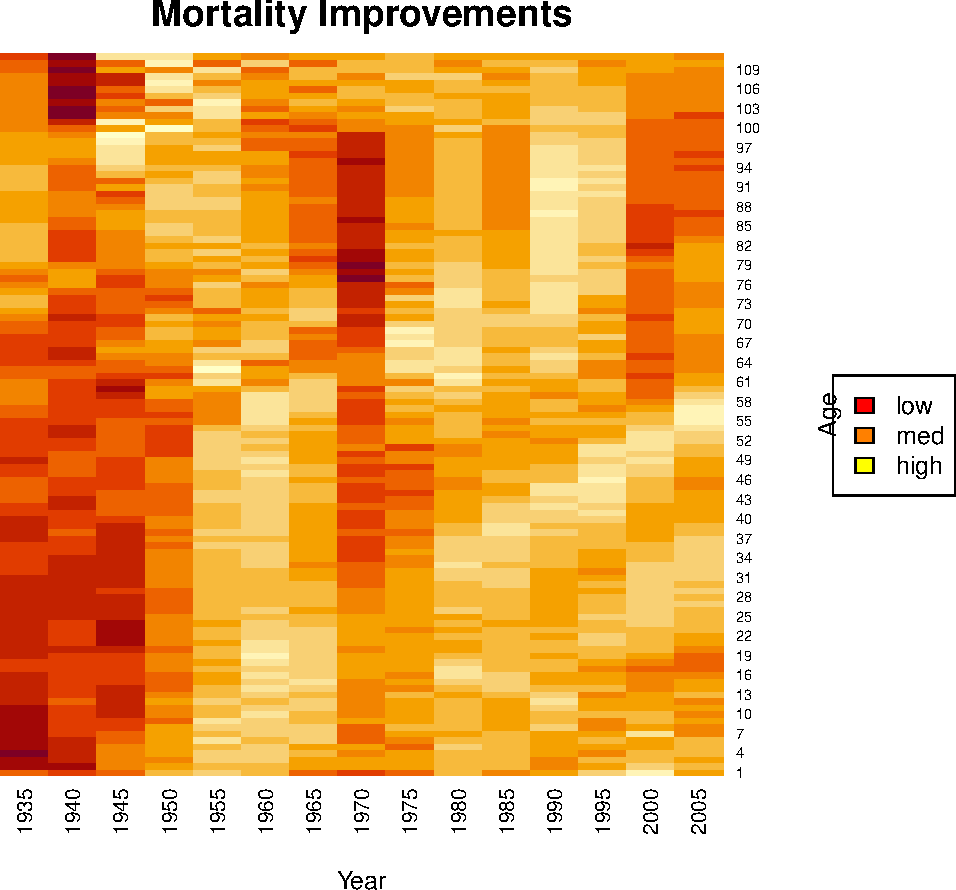
\includegraphics{LifeCon_files/figure-latex/MortImpHeatFiga-1} 

}

\caption{\textbf{Heatmap for Mortality Improvements for U.S. Females Across Times and Ages}}\label{fig:MortImpHeatFiga}
\end{figure}

As we can see, mortality improvements vary quiet a bit over time and age, but we do see quite substantial improvements for low to medium ages in the more recent past. One interesting aspect here is that clearly there is a relationship between time and age. For a certain birth cohort, as time passes, the individuals will age. In particular, we identify the diagonals in the heatmap with a certain birth cohort, and we observe some distinct relationships on the diagonals. For instance, the cohort if individuals born around 1950 appears to experience quite substantial improvements across all years of age, which could be due to environmental or socio-economic factors.

One simple way of accounting for improvements and forecasting mortality into the future are so-called \emph{single factor mortality improvement models}, i.e.~models where \(\varphi(x,t)\) only depends on \(x\) -- let's write \(\varphi_x\). With that, the above equation becomes:
\[
q_{x,t}= q_{x,t-1}\times (1- \varphi_x),
\]
or, generalizing:
\[
q_{x,t} = q_{x,0}\times (1-\varphi_x)^t
\]

To obtain suitable improvement factors for making projections, for deriving \(\phi_x\) let's average across years under consideration and smooth across ages using a simple local regression smoother:

R Code For Figure

\hypertarget{toggleCode.Mortalityux20Improvementux20Factorsux20forux20USux20Females}{}
\begin{Shaded}
\begin{Highlighting}[]
\NormalTok{phi_x <-}\StringTok{ }\KeywordTok{rep}\NormalTok{(}\DecValTok{0}\NormalTok{,}\DecValTok{111}\NormalTok{)}
\ControlFlowTok{for}\NormalTok{ (x }\ControlFlowTok{in} \DecValTok{1}\OperatorTok{:}\DecValTok{111}\NormalTok{)\{}
\NormalTok{  phi_x[x] <-}\StringTok{ }\KeywordTok{mean}\NormalTok{(phi[x,])}
\NormalTok{\}}
\NormalTok{ages <-}\StringTok{ }\DecValTok{1}\OperatorTok{:}\DecValTok{111}
\NormalTok{lo <-}\StringTok{ }\KeywordTok{loess}\NormalTok{(phi_x }\OperatorTok{~}\StringTok{ }\NormalTok{ages)}
\KeywordTok{plot}\NormalTok{(phi_x, }\DataTypeTok{type =} \StringTok{"l"}\NormalTok{, }\DataTypeTok{lwd =} \DecValTok{5}\NormalTok{, }\DataTypeTok{col =} \StringTok{"red"}\NormalTok{, }\DataTypeTok{main=}\StringTok{"Mortality Improvement Factors, US Females"}\NormalTok{, }\DataTypeTok{xlab =} \StringTok{"age"}\NormalTok{, }\DataTypeTok{ylab =} \StringTok{"phi"}\NormalTok{)}
\KeywordTok{lines}\NormalTok{(}\KeywordTok{predict}\NormalTok{(lo), }\DataTypeTok{col=}\StringTok{'blue'}\NormalTok{, }\DataTypeTok{lwd=}\DecValTok{2}\NormalTok{)}
\NormalTok{phi_x <-}\StringTok{ }\KeywordTok{predict}\NormalTok{(lo)}
\end{Highlighting}
\end{Shaded}



\begin{figure}

{\centering 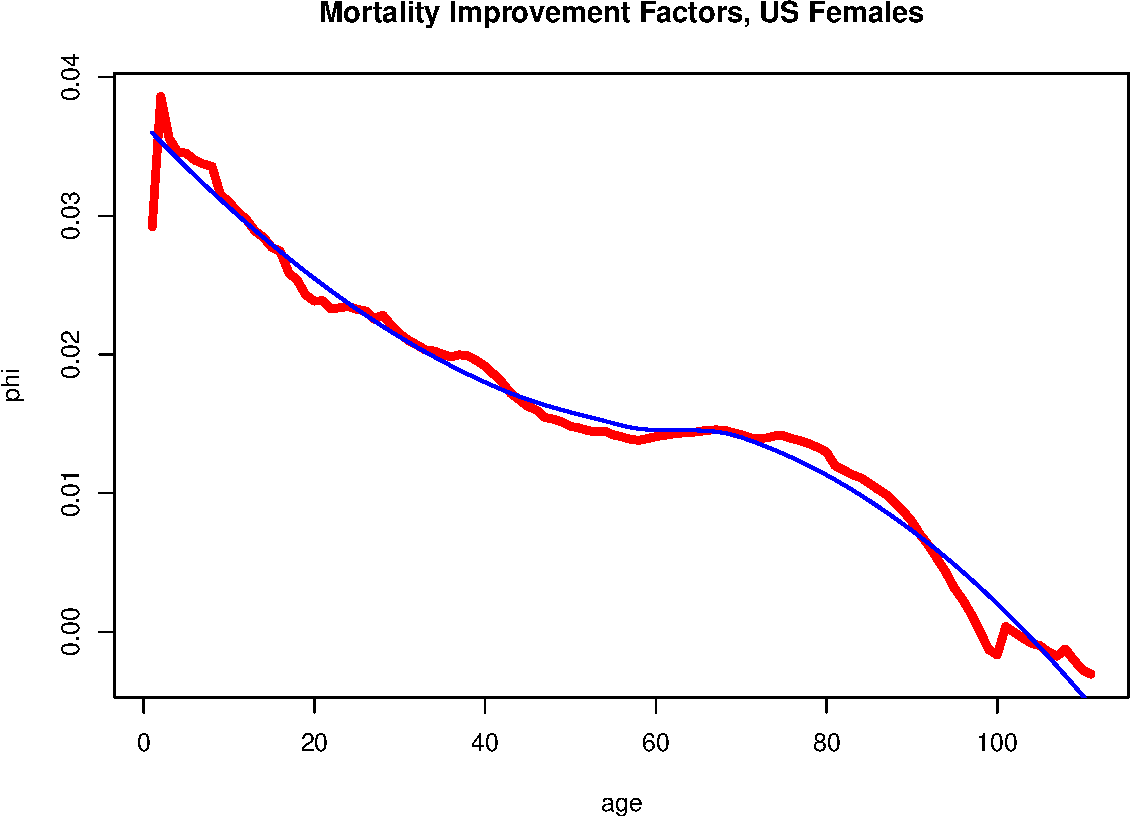
\includegraphics{LifeCon_files/figure-latex/MortImpFacsa-1} 

}

\caption{\textbf{Mortality Improvement Factors for U.S. Females}}\label{fig:MortImpFacsa}
\end{figure}

It is important to stress that we are no longer in the age-only model, since now a seventy-year-old today and a seventy-year-old ten years from now. However, as we already indicated in Section \ref{S:ModelOnlyAge}, in this case of a bivariate \(\bf{x}\) where one of the covariates---year of birth---is immutable for an individual, we can still rely on the same ideas as in the age-only model. Hence, in particular, we can still defined life tables, although life tables will now be two dimensional since we will have different \(q_{x,t}\) for every year \(t\).

To illustrate, let us create a \emph{cohort life table} for fifty year old females \emph{now}, where for simplicity we denote the current time by \(t=0\) (corresponding to the timing of the period life table we created). Then we can obtain prospective mortality probabilities \(q_{50+t,t}\) via:
\[
q_{50+t,t} = q_{50+t,0} \times (1-\varphi_{50+t})^t.
\]
Let us plot these \emph{cohort mortality probabilities} and compare them to our \emph{period mortality probabilities}:

R Code For Figure

\hypertarget{toggleCode.Cohortux20vs.ux20Periodux20q_xux20forux2050-yearux20oldux20U.S.ux20females}{}
\begin{Shaded}
\begin{Highlighting}[]
\NormalTok{q_50plusx <-}\StringTok{ }\KeywordTok{rep}\NormalTok{(}\DecValTok{0}\NormalTok{,}\DecValTok{61}\NormalTok{)}
\ControlFlowTok{for}\NormalTok{ (i }\ControlFlowTok{in} \DecValTok{1}\OperatorTok{:}\DecValTok{61}\NormalTok{)\{}
\NormalTok{  q_50plusx[i] <-}\StringTok{ }\NormalTok{us_mx_fem_}\DecValTok{2014}\NormalTok{[}\DecValTok{50}\OperatorTok{+}\NormalTok{i,}\DecValTok{4}\NormalTok{] }\OperatorTok{*}\StringTok{ }\NormalTok{(}\DecValTok{1} \OperatorTok{-}\StringTok{ }\NormalTok{phi_x[}\DecValTok{50}\OperatorTok{+}\NormalTok{i])}\OperatorTok{^}\NormalTok{(i}\DecValTok{-1}\NormalTok{)}
\NormalTok{\}}
\KeywordTok{plot}\NormalTok{(}\DecValTok{50}\OperatorTok{:}\DecValTok{99}\NormalTok{,q_50plusx[}\DecValTok{1}\OperatorTok{:}\DecValTok{50}\NormalTok{], }\DataTypeTok{type =} \StringTok{"l"}\NormalTok{, }\DataTypeTok{lwd =} \DecValTok{2}\NormalTok{, }\DataTypeTok{col =} \StringTok{"red"}\NormalTok{, }\DataTypeTok{main=}\StringTok{"q_x comparison"}\NormalTok{, }\DataTypeTok{xlab =} \StringTok{"age"}\NormalTok{)}
\KeywordTok{lines}\NormalTok{(}\DecValTok{50}\OperatorTok{:}\DecValTok{99}\NormalTok{,us_mx_fem_}\DecValTok{2014}\NormalTok{[}\DecValTok{51}\OperatorTok{:}\DecValTok{100}\NormalTok{,}\DecValTok{4}\NormalTok{], }\DataTypeTok{col =} \StringTok{"blue"}\NormalTok{, }\DataTypeTok{lwd =} \DecValTok{2}\NormalTok{)}
\end{Highlighting}
\end{Shaded}



\begin{figure}

{\centering 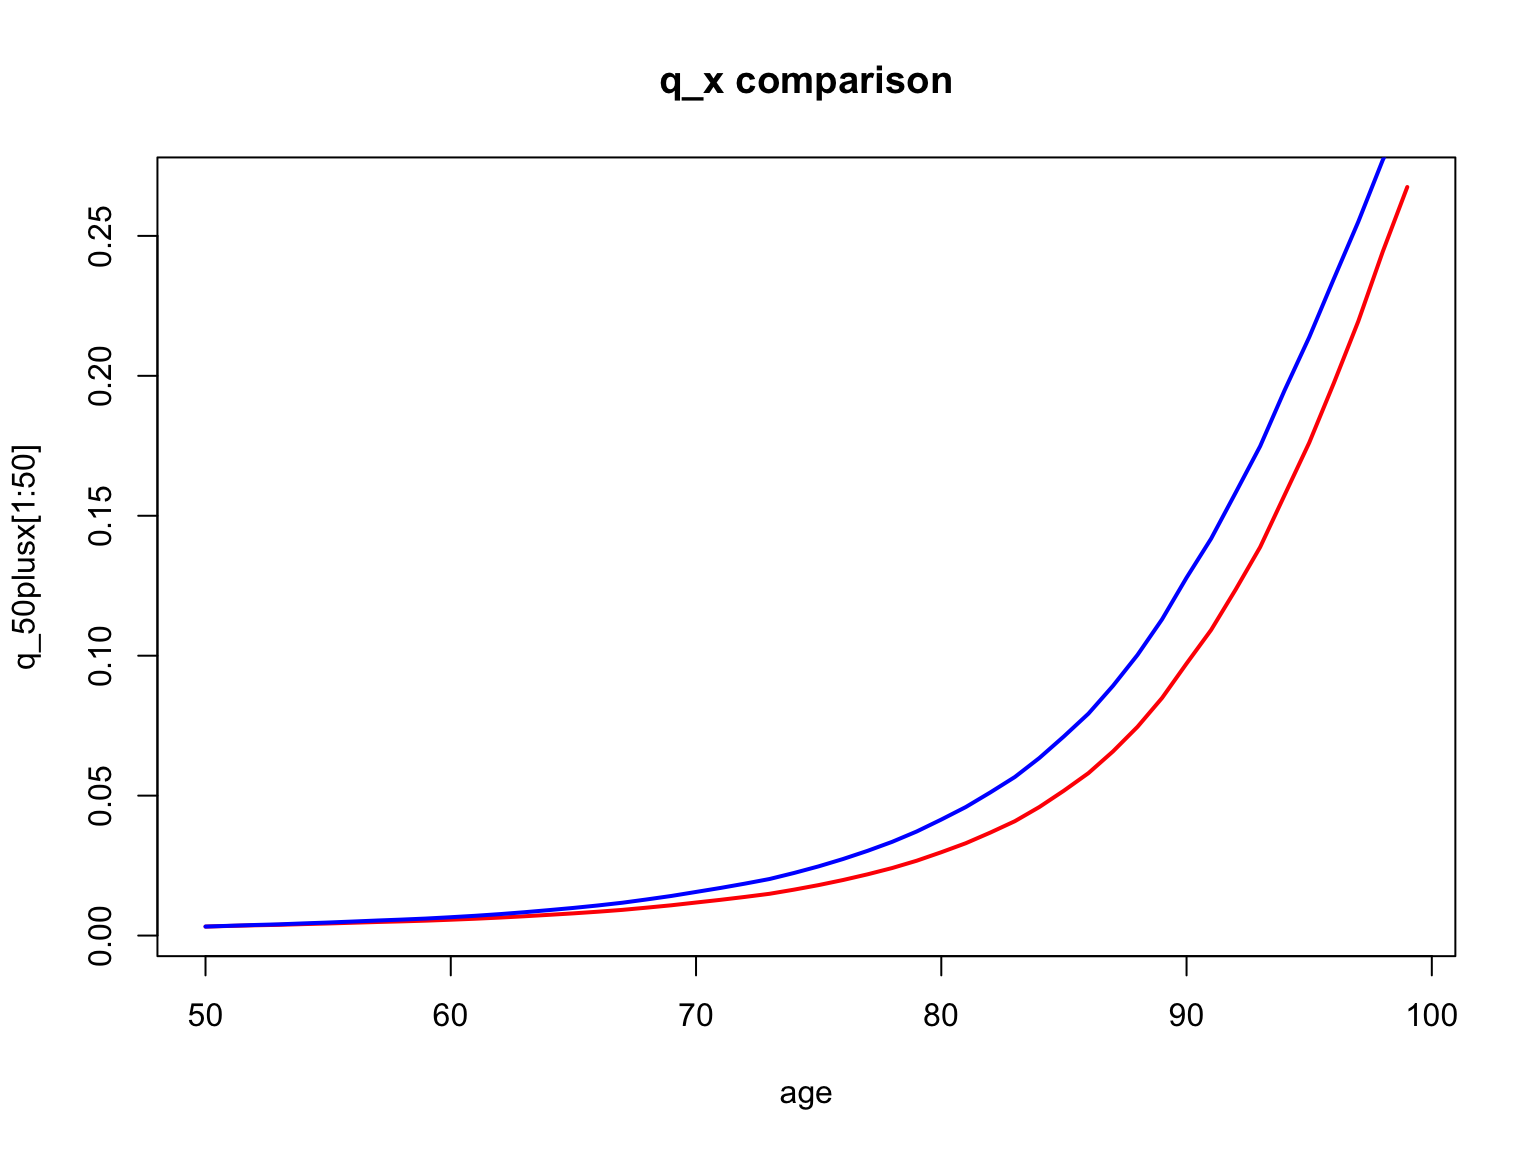
\includegraphics{LifeCon_files/figure-latex/CohortvsPeriodqxa-1} 

}

\caption{\textbf{Cohort (red) vs.~Period (blue) q\_x for 50-year old U.S. females}}\label{fig:CohortvsPeriodqxa}
\end{figure}

Evidently the cohort mortality probabilities are lower than the period mortality probabilities, as we incorporate mortality improvements. Of course, this comes with the assumption that the future mortality evolution will be similar to that in the past. While critical, it is not possible to make a projections without any assumption, and reliance on a period table is equivalent to assuming there will not be improvements whatsoever. These \(q_{50+t,t}\) and now be relied on for determining actuarial quantities just as in the previous section.

If we use all ages \(x\) today and determine corresponding \(q_{x+t,t}\), \(t=0,1,2,...\), \(x=0,1,2,...\), just as above, we obtain a two-dimensional \emph{cohort} or \emph{projective life table}. In particular, we can consider newborn females and determine their (curtate) life expectancy, resulting in:

R Code For Cohort Life Expectancy

\hypertarget{toggleCode.Cohortux20Lifeux20Expectancyux20forux20U.S.ux20females}{}
\begin{Shaded}
\begin{Highlighting}[]
\NormalTok{q_0plusx <-}\StringTok{ }\KeywordTok{rep}\NormalTok{(}\DecValTok{0}\NormalTok{,}\DecValTok{110}\NormalTok{)}
\ControlFlowTok{for}\NormalTok{ (i }\ControlFlowTok{in} \DecValTok{1}\OperatorTok{:}\DecValTok{110}\NormalTok{)\{}
\NormalTok{q_0plusx[i] <-}\StringTok{ }\NormalTok{us_mx_fem_}\DecValTok{2014}\NormalTok{[i,}\DecValTok{4}\NormalTok{] }\OperatorTok{*}\StringTok{ }\NormalTok{(}\DecValTok{1} \OperatorTok{-}\StringTok{ }\NormalTok{phi_x[i])}\OperatorTok{^}\NormalTok{(i}\DecValTok{-1}\NormalTok{)}
\NormalTok{\}}
\NormalTok{kP0_i <-}\StringTok{ }\KeywordTok{rep}\NormalTok{(}\DecValTok{0}\NormalTok{,}\DecValTok{110}\NormalTok{)}
\NormalTok{kP0_i[}\DecValTok{1}\NormalTok{] <-}\StringTok{ }\DecValTok{1} 
\ControlFlowTok{for}\NormalTok{ (i }\ControlFlowTok{in} \DecValTok{2}\OperatorTok{:}\DecValTok{110}\NormalTok{)\{}
\NormalTok{  kP0_i[i] <-}\StringTok{ }\NormalTok{kP0_i[i}\DecValTok{-1}\NormalTok{] }\OperatorTok{*}\StringTok{ }\NormalTok{(}\DecValTok{1} \OperatorTok{-}\StringTok{ }\NormalTok{q_0plusx[i}\DecValTok{-1}\NormalTok{])}
\NormalTok{\}}
\NormalTok{e_0Coh <-}\StringTok{ }\KeywordTok{sum}\NormalTok{(kP0_i) }\OperatorTok{-}\StringTok{ }\DecValTok{1} 
\end{Highlighting}
\end{Shaded}

\begin{Shaded}
\begin{Highlighting}[]
\NormalTok{e_0Coh}
\end{Highlighting}
\end{Shaded}

\begin{verbatim}
[1] 88.1249429
\end{verbatim}

Hence, due to mortality improvements, our projected life expectancy is substantially larger than that based on our period table of 80.8 years from Section \ref{S:LifeTabRec} or that based U.S. national statistics of 81.1 from Section \ref{S:DataLifeExp}.

\hypertarget{S:NonParamSurv}{%
\section{Non-parametric survival estimation}\label{S:NonParamSurv}}

The previous section introduced life tables as a (discretized) representation of a \emph{non-parametric} survival function in the age-only model. We also showed how to compile a period life table based on (population) mortality count data, essentially by deriving mortality rates from a given time window.

How can we determine a life table---or, more generally, a survival function---from mortality data at the individual level, which an insurance company has available, such as the dataset we introduced in Section \ref{S:IndivMortData}? One approach is to follow a similar path as in the previous section, by translating the individual outcomes into counts and the proceeding similarly. However, the number of deaths within a given year and at a certain age may be rather limited for a single company's portfolio, especially when constraining the individuals to a certain subgroup determined by sex, smoking status, health, etc. Therefore, in practice life tables are often compiled at the industry level, such as within the so-called \href{https://www.soa.org/resources/experience-studies/2015/2015-valuation-basic-tables/}{Valuation Basic Table} by the American Academy of Actuaries.

The current section discusses non-parametric estimation of survival functions based on a individual level mortality dataset that inlcudes truncated and censored data, where we rely on the dataset from Section \ref{S:IndivMortData} for illustration. In anaology to the previous section, the setting here is the age-only approach, i.e., we determine one survival curve that reflects mortality as a function of age. However, by constraining the dataset to certain subrgoups, we can generate different survival curves for these different subgroups. We commence by introducing the \emph{Kaplan-Meier} (product limit) approach for estimating the survival curve and then discuss the \emph{Nelson-Aalen} estimator for the cumulative hazard.

\hypertarget{kaplan-meier-estimate}{%
\subsection{Kaplan-Meier Estimate}\label{kaplan-meier-estimate}}

The intuition for the Kaplan-Meier estimate is straightforward. Recall from Section \ref{S:ModelOnlyAge} that in the age-only model, for the survival function for \(x\)-year-olds we have:
\[
S_x(0) = 1 \text{ and } S_x(t+1) = S_x(t) \times p_{x+t} 
\]
for integer \(x\) and \(t\). Furthermore, from the previous section on life tables, given information on exposures \(l_{x+t}\) and deaths \(d_{x+t}\) at time \(x+t\), we estimate:
\[
p_{x+t} = 1 - \frac{d_{x+t}}{l_{x+t}} \Longrightarrow S_x(t+1) = S_x(t) \times \left(1 - \frac{d_{x+t}}{l_{x+t}}\right).
\]
The Kaplan-Meier estimate uses the exact same relationship, although it takes into account that in the context of right-censored individual mortality data, potential exposures at each death time may be different. That is, \(l_{x+t}\) in this equation should be interpreted as the total number of individuals at risk of dying at time \(x+t\). This number will change across time because individuals die \emph{and} because of right-censoring, so indviduals falling outside of the observation window. As a consequence, the survival function is updated whenever there is a death event, and the number of corresponding exposures is recalculated at every point. For additional details as well as a discussion of how to determine the variance of the estimate, we refer to \href{https://openacttexts.github.io/Loss-Data-Analytics/C-ModelSelection.html\#nonparametric-estimation-using-modified-data}{Section 4.3.2 in Loss Data Analystics}.

An important caveat to the application of the Kaplan-Meier estimate is that all exposures are treated alike in the context of the age-only model. Hence, individuals of the same age at different times are entering the survival curve estimate. In particular, the \emph{set} of observations that is used for estimating the survival curve determines the population for which the survival curve is relevant.

In \texttt{R}, we can use the library \texttt{survival}. We estimate survival curves based on our insurer dataset from Section \ref{S:IndivMortData} for ages 30, 40, and 50, where we compare survival curves for males, females, and the aggregate curves. Let us plot them curves.

R Code For Figure

\hypertarget{toggleCode.Kaplan-Meierux20Estimatesux20ofux20Survivalux20Curvesux20forux20agesux2030ux2cux2040ux2cux2050}{}
\begin{Shaded}
\begin{Highlighting}[]
\KeywordTok{library}\NormalTok{(data.table)}
\KeywordTok{library}\NormalTok{(survival)}
\NormalTok{insdatatmp <-}\StringTok{ }\KeywordTok{fread}\NormalTok{(}\StringTok{"Data/SyntheticInsurerData.csv"}\NormalTok{,}\DataTypeTok{data.table=}\OtherTok{FALSE}\NormalTok{)}

\CommentTok{# computations for individuals aged 50 }
\NormalTok{ageX <-}\StringTok{ }\DecValTok{50}
\CommentTok{#FEMALE}
\NormalTok{sexX <-}\StringTok{ }\DecValTok{0} \CommentTok{# 0 for female, 1 for male}
\NormalTok{setdata <-}\StringTok{ }\NormalTok{insdatatmp[}\KeywordTok{which}\NormalTok{(insdatatmp}\OperatorTok{$}\NormalTok{Age}\OperatorTok{+}\KeywordTok{floor}\NormalTok{(insdatatmp}\OperatorTok{$}\NormalTok{Time_of_death) }\OperatorTok{>=}\NormalTok{ageX }\OperatorTok{&}\StringTok{ }\NormalTok{insdatatmp}\OperatorTok{$}\NormalTok{Age }\OperatorTok{<=}\StringTok{ }\NormalTok{ageX }\OperatorTok{&}\StringTok{ }\NormalTok{insdatatmp}\OperatorTok{$}\NormalTok{Sex}\OperatorTok{==}\NormalTok{sexX),]}
\NormalTok{time <-}\StringTok{ }\KeywordTok{rep}\NormalTok{(}\DecValTok{0}\NormalTok{,}\KeywordTok{nrow}\NormalTok{(setdata))}
\NormalTok{status<-}\DecValTok{1}\OperatorTok{*}\NormalTok{(setdata}\OperatorTok{$}\NormalTok{Claim }\OperatorTok{==}\StringTok{ "YES"}\NormalTok{) }\CommentTok{# 0 for Censored data observations (i.e. with no claims and Claim=="No"), 1 for non-Censored observations -- setting for Survfit function}
\NormalTok{time <-}\StringTok{ }\NormalTok{setdata}\OperatorTok{$}\NormalTok{Time_of_death }\OperatorTok{-}\StringTok{ }\NormalTok{(}\KeywordTok{rep}\NormalTok{(ageX,}\KeywordTok{nrow}\NormalTok{(setdata))}\OperatorTok{-}\NormalTok{setdata}\OperatorTok{$}\NormalTok{Age)}
\NormalTok{fit_KM_}\DecValTok{50}\NormalTok{_F <-}\StringTok{ }\KeywordTok{survfit}\NormalTok{(}\KeywordTok{Surv}\NormalTok{(time,status) }\OperatorTok{~}\StringTok{ }\DecValTok{1}\NormalTok{, }\DataTypeTok{type=}\StringTok{'kaplan-meier'}\NormalTok{) }\CommentTok{# Kaplan-Meier estimator}
\CommentTok{#MALE}
\NormalTok{sexX <-}\StringTok{ }\DecValTok{1} \CommentTok{# 0 for female, 1 for male}
\NormalTok{setdata <-}\StringTok{ }\NormalTok{insdatatmp[}\KeywordTok{which}\NormalTok{(insdatatmp}\OperatorTok{$}\NormalTok{Age}\OperatorTok{+}\KeywordTok{floor}\NormalTok{(insdatatmp}\OperatorTok{$}\NormalTok{Time_of_death) }\OperatorTok{>=}\NormalTok{ageX }\OperatorTok{&}\StringTok{ }\NormalTok{insdatatmp}\OperatorTok{$}\NormalTok{Age }\OperatorTok{<=}\StringTok{ }\NormalTok{ageX }\OperatorTok{&}\StringTok{ }\NormalTok{insdatatmp}\OperatorTok{$}\NormalTok{Sex}\OperatorTok{==}\NormalTok{sexX),]}
\NormalTok{time <-}\StringTok{ }\KeywordTok{rep}\NormalTok{(}\DecValTok{0}\NormalTok{,}\KeywordTok{nrow}\NormalTok{(setdata))}
\NormalTok{status<-}\DecValTok{1}\OperatorTok{*}\NormalTok{(setdata}\OperatorTok{$}\NormalTok{Claim }\OperatorTok{==}\StringTok{ "YES"}\NormalTok{) }\CommentTok{# 0 for Censored data observations (i.e. with no claims and Claim=="No"), 1 for non-Censored observations -- setting for Survfit function}
\NormalTok{time <-}\StringTok{ }\NormalTok{setdata}\OperatorTok{$}\NormalTok{Time_of_death }\OperatorTok{-}\StringTok{ }\NormalTok{(}\KeywordTok{rep}\NormalTok{(ageX,}\KeywordTok{nrow}\NormalTok{(setdata))}\OperatorTok{-}\NormalTok{setdata}\OperatorTok{$}\NormalTok{Age)}
\NormalTok{fit_KM_}\DecValTok{50}\NormalTok{_M <-}\StringTok{ }\KeywordTok{survfit}\NormalTok{(}\KeywordTok{Surv}\NormalTok{(time,status) }\OperatorTok{~}\StringTok{ }\DecValTok{1}\NormalTok{, }\DataTypeTok{type=}\StringTok{'kaplan-meier'}\NormalTok{)}
\CommentTok{#AGGREGATE}
\NormalTok{setdata <-}\StringTok{ }\NormalTok{insdatatmp[}\KeywordTok{which}\NormalTok{(insdatatmp}\OperatorTok{$}\NormalTok{Age}\OperatorTok{+}\KeywordTok{floor}\NormalTok{(insdatatmp}\OperatorTok{$}\NormalTok{Time_of_death) }\OperatorTok{>=}\NormalTok{ageX }\OperatorTok{&}\StringTok{ }\NormalTok{insdatatmp}\OperatorTok{$}\NormalTok{Age }\OperatorTok{<=}\StringTok{ }\NormalTok{ageX),]}
\NormalTok{time <-}\StringTok{ }\KeywordTok{rep}\NormalTok{(}\DecValTok{0}\NormalTok{,}\KeywordTok{nrow}\NormalTok{(setdata))}
\NormalTok{status<-}\DecValTok{1}\OperatorTok{*}\NormalTok{(setdata}\OperatorTok{$}\NormalTok{Claim }\OperatorTok{==}\StringTok{ "YES"}\NormalTok{) }\CommentTok{# 0 for Censored data observations (i.e. with no claims and Claim=="No"), 1 for non-Censored observations -- setting for Survfit function}
\NormalTok{time <-}\StringTok{ }\NormalTok{setdata}\OperatorTok{$}\NormalTok{Time_of_death }\OperatorTok{-}\StringTok{ }\NormalTok{(}\KeywordTok{rep}\NormalTok{(ageX,}\KeywordTok{nrow}\NormalTok{(setdata))}\OperatorTok{-}\NormalTok{setdata}\OperatorTok{$}\NormalTok{Age)}
\NormalTok{fit_KM_}\DecValTok{50}\NormalTok{_All <-}\StringTok{ }\KeywordTok{survfit}\NormalTok{(}\KeywordTok{Surv}\NormalTok{(time,status) }\OperatorTok{~}\StringTok{ }\DecValTok{1}\NormalTok{, }\DataTypeTok{type=}\StringTok{'kaplan-meier'}\NormalTok{)}

\CommentTok{# computations for individuals aged 40 }
\NormalTok{ageX <-}\StringTok{ }\DecValTok{40}
\CommentTok{#FEMALE}
\NormalTok{sexX <-}\StringTok{ }\DecValTok{0} \CommentTok{# 0 for female, 1 for male}
\NormalTok{setdata <-}\StringTok{ }\NormalTok{insdatatmp[}\KeywordTok{which}\NormalTok{(insdatatmp}\OperatorTok{$}\NormalTok{Age}\OperatorTok{+}\KeywordTok{floor}\NormalTok{(insdatatmp}\OperatorTok{$}\NormalTok{Time_of_death) }\OperatorTok{>=}\NormalTok{ageX }\OperatorTok{&}\StringTok{ }\NormalTok{insdatatmp}\OperatorTok{$}\NormalTok{Age }\OperatorTok{<=}\StringTok{ }\NormalTok{ageX }\OperatorTok{&}\StringTok{ }\NormalTok{insdatatmp}\OperatorTok{$}\NormalTok{Sex}\OperatorTok{==}\NormalTok{sexX),]}
\NormalTok{time <-}\StringTok{ }\KeywordTok{rep}\NormalTok{(}\DecValTok{0}\NormalTok{,}\KeywordTok{nrow}\NormalTok{(setdata))}
\NormalTok{status<-}\DecValTok{1}\OperatorTok{*}\NormalTok{(setdata}\OperatorTok{$}\NormalTok{Claim }\OperatorTok{==}\StringTok{ "YES"}\NormalTok{) }\CommentTok{# 0 for Censored data observations (i.e. with no claims and Claim=="No"), 1 for non-Censored observations -- setting for Survfit function}
\NormalTok{time <-}\StringTok{ }\NormalTok{setdata}\OperatorTok{$}\NormalTok{Time_of_death }\OperatorTok{-}\StringTok{ }\NormalTok{(}\KeywordTok{rep}\NormalTok{(ageX,}\KeywordTok{nrow}\NormalTok{(setdata))}\OperatorTok{-}\NormalTok{setdata}\OperatorTok{$}\NormalTok{Age)}
\NormalTok{fit_KM_}\DecValTok{40}\NormalTok{_F <-}\StringTok{ }\KeywordTok{survfit}\NormalTok{(}\KeywordTok{Surv}\NormalTok{(time,status) }\OperatorTok{~}\StringTok{ }\DecValTok{1}\NormalTok{, }\DataTypeTok{type=}\StringTok{'kaplan-meier'}\NormalTok{) }\CommentTok{# Kaplan-Meier estimator}
\CommentTok{#MALE}
\NormalTok{sexX <-}\StringTok{ }\DecValTok{1} \CommentTok{# 0 for female, 1 for male}
\NormalTok{setdata <-}\StringTok{ }\NormalTok{insdatatmp[}\KeywordTok{which}\NormalTok{(insdatatmp}\OperatorTok{$}\NormalTok{Age}\OperatorTok{+}\KeywordTok{floor}\NormalTok{(insdatatmp}\OperatorTok{$}\NormalTok{Time_of_death) }\OperatorTok{>=}\NormalTok{ageX }\OperatorTok{&}\StringTok{ }\NormalTok{insdatatmp}\OperatorTok{$}\NormalTok{Age }\OperatorTok{<=}\StringTok{ }\NormalTok{ageX }\OperatorTok{&}\StringTok{ }\NormalTok{insdatatmp}\OperatorTok{$}\NormalTok{Sex}\OperatorTok{==}\NormalTok{sexX),]}
\NormalTok{time <-}\StringTok{ }\KeywordTok{rep}\NormalTok{(}\DecValTok{0}\NormalTok{,}\KeywordTok{nrow}\NormalTok{(setdata))}
\NormalTok{status<-}\DecValTok{1}\OperatorTok{*}\NormalTok{(setdata}\OperatorTok{$}\NormalTok{Claim }\OperatorTok{==}\StringTok{ "YES"}\NormalTok{) }\CommentTok{# 0 for Censored data observations (i.e. with no claims and Claim=="No"), 1 for non-Censored observations -- setting for Survfit function}
\NormalTok{time <-}\StringTok{ }\NormalTok{setdata}\OperatorTok{$}\NormalTok{Time_of_death }\OperatorTok{-}\StringTok{ }\NormalTok{(}\KeywordTok{rep}\NormalTok{(ageX,}\KeywordTok{nrow}\NormalTok{(setdata))}\OperatorTok{-}\NormalTok{setdata}\OperatorTok{$}\NormalTok{Age)}
\NormalTok{fit_KM_}\DecValTok{40}\NormalTok{_M <-}\StringTok{ }\KeywordTok{survfit}\NormalTok{(}\KeywordTok{Surv}\NormalTok{(time,status) }\OperatorTok{~}\StringTok{ }\DecValTok{1}\NormalTok{, }\DataTypeTok{type=}\StringTok{'kaplan-meier'}\NormalTok{)}
\CommentTok{#AGGREGATE}
\NormalTok{setdata <-}\StringTok{ }\NormalTok{insdatatmp[}\KeywordTok{which}\NormalTok{(insdatatmp}\OperatorTok{$}\NormalTok{Age}\OperatorTok{+}\KeywordTok{floor}\NormalTok{(insdatatmp}\OperatorTok{$}\NormalTok{Time_of_death) }\OperatorTok{>=}\NormalTok{ageX }\OperatorTok{&}\StringTok{ }\NormalTok{insdatatmp}\OperatorTok{$}\NormalTok{Age }\OperatorTok{<=}\StringTok{ }\NormalTok{ageX),]}
\NormalTok{time <-}\StringTok{ }\KeywordTok{rep}\NormalTok{(}\DecValTok{0}\NormalTok{,}\KeywordTok{nrow}\NormalTok{(setdata))}
\NormalTok{status<-}\DecValTok{1}\OperatorTok{*}\NormalTok{(setdata}\OperatorTok{$}\NormalTok{Claim }\OperatorTok{==}\StringTok{ "YES"}\NormalTok{) }\CommentTok{# 0 for Censored data observations (i.e. with no claims and Claim=="No"), 1 for non-Censored observations -- setting for Survfit function}
\NormalTok{time <-}\StringTok{ }\NormalTok{setdata}\OperatorTok{$}\NormalTok{Time_of_death }\OperatorTok{-}\StringTok{ }\NormalTok{(}\KeywordTok{rep}\NormalTok{(ageX,}\KeywordTok{nrow}\NormalTok{(setdata))}\OperatorTok{-}\NormalTok{setdata}\OperatorTok{$}\NormalTok{Age)}
\NormalTok{fit_KM_}\DecValTok{40}\NormalTok{_All <-}\StringTok{ }\KeywordTok{survfit}\NormalTok{(}\KeywordTok{Surv}\NormalTok{(time,status) }\OperatorTok{~}\StringTok{ }\DecValTok{1}\NormalTok{, }\DataTypeTok{type=}\StringTok{'kaplan-meier'}\NormalTok{)}

\CommentTok{# computations for individuals aged 30 }
\NormalTok{ageX <-}\StringTok{ }\DecValTok{30}
\CommentTok{#FEMALE}
\NormalTok{sexX <-}\StringTok{ }\DecValTok{0} \CommentTok{# 0 for female, 1 for male}
\NormalTok{setdata <-}\StringTok{ }\NormalTok{insdatatmp[}\KeywordTok{which}\NormalTok{(insdatatmp}\OperatorTok{$}\NormalTok{Age}\OperatorTok{+}\KeywordTok{floor}\NormalTok{(insdatatmp}\OperatorTok{$}\NormalTok{Time_of_death) }\OperatorTok{>=}\NormalTok{ageX }\OperatorTok{&}\StringTok{ }\NormalTok{insdatatmp}\OperatorTok{$}\NormalTok{Age }\OperatorTok{<=}\StringTok{ }\NormalTok{ageX }\OperatorTok{&}\StringTok{ }\NormalTok{insdatatmp}\OperatorTok{$}\NormalTok{Sex}\OperatorTok{==}\NormalTok{sexX),]}
\NormalTok{time <-}\StringTok{ }\KeywordTok{rep}\NormalTok{(}\DecValTok{0}\NormalTok{,}\KeywordTok{nrow}\NormalTok{(setdata))}
\NormalTok{status<-}\DecValTok{1}\OperatorTok{*}\NormalTok{(setdata}\OperatorTok{$}\NormalTok{Claim }\OperatorTok{==}\StringTok{ "YES"}\NormalTok{) }\CommentTok{# 0 for Censored data observations (i.e. with no claims and Claim=="No"), 1 for non-Censored observations -- setting for Survfit function}
\NormalTok{time <-}\StringTok{ }\NormalTok{setdata}\OperatorTok{$}\NormalTok{Time_of_death }\OperatorTok{-}\StringTok{ }\NormalTok{(}\KeywordTok{rep}\NormalTok{(ageX,}\KeywordTok{nrow}\NormalTok{(setdata))}\OperatorTok{-}\NormalTok{setdata}\OperatorTok{$}\NormalTok{Age)}
\NormalTok{fit_KM_}\DecValTok{30}\NormalTok{_F <-}\StringTok{ }\KeywordTok{survfit}\NormalTok{(}\KeywordTok{Surv}\NormalTok{(time,status) }\OperatorTok{~}\StringTok{ }\DecValTok{1}\NormalTok{, }\DataTypeTok{type=}\StringTok{'kaplan-meier'}\NormalTok{) }\CommentTok{# Kaplan-Meier estimator}
\CommentTok{#MALE}
\NormalTok{sexX <-}\StringTok{ }\DecValTok{1} \CommentTok{# 0 for female, 1 for male}
\NormalTok{setdata <-}\StringTok{ }\NormalTok{insdatatmp[}\KeywordTok{which}\NormalTok{(insdatatmp}\OperatorTok{$}\NormalTok{Age}\OperatorTok{+}\KeywordTok{floor}\NormalTok{(insdatatmp}\OperatorTok{$}\NormalTok{Time_of_death) }\OperatorTok{>=}\NormalTok{ageX }\OperatorTok{&}\StringTok{ }\NormalTok{insdatatmp}\OperatorTok{$}\NormalTok{Age }\OperatorTok{<=}\StringTok{ }\NormalTok{ageX }\OperatorTok{&}\StringTok{ }\NormalTok{insdatatmp}\OperatorTok{$}\NormalTok{Sex}\OperatorTok{==}\NormalTok{sexX),]}
\NormalTok{time <-}\StringTok{ }\KeywordTok{rep}\NormalTok{(}\DecValTok{0}\NormalTok{,}\KeywordTok{nrow}\NormalTok{(setdata))}
\NormalTok{status<-}\DecValTok{1}\OperatorTok{*}\NormalTok{(setdata}\OperatorTok{$}\NormalTok{Claim }\OperatorTok{==}\StringTok{ "YES"}\NormalTok{) }\CommentTok{# 0 for Censored data observations (i.e. with no claims and Claim=="No"), 1 for non-Censored observations -- setting for Survfit function}
\NormalTok{time <-}\StringTok{ }\NormalTok{setdata}\OperatorTok{$}\NormalTok{Time_of_death }\OperatorTok{-}\StringTok{ }\NormalTok{(}\KeywordTok{rep}\NormalTok{(ageX,}\KeywordTok{nrow}\NormalTok{(setdata))}\OperatorTok{-}\NormalTok{setdata}\OperatorTok{$}\NormalTok{Age)}
\NormalTok{fit_KM_}\DecValTok{30}\NormalTok{_M <-}\StringTok{ }\KeywordTok{survfit}\NormalTok{(}\KeywordTok{Surv}\NormalTok{(time,status) }\OperatorTok{~}\StringTok{ }\DecValTok{1}\NormalTok{, }\DataTypeTok{type=}\StringTok{'kaplan-meier'}\NormalTok{)}
\CommentTok{#AGGREGATE}
\NormalTok{setdata <-}\StringTok{ }\NormalTok{insdatatmp[}\KeywordTok{which}\NormalTok{(insdatatmp}\OperatorTok{$}\NormalTok{Age}\OperatorTok{+}\KeywordTok{floor}\NormalTok{(insdatatmp}\OperatorTok{$}\NormalTok{Time_of_death) }\OperatorTok{>=}\NormalTok{ageX }\OperatorTok{&}\StringTok{ }\NormalTok{insdatatmp}\OperatorTok{$}\NormalTok{Age }\OperatorTok{<=}\StringTok{ }\NormalTok{ageX),]}
\NormalTok{time <-}\StringTok{ }\KeywordTok{rep}\NormalTok{(}\DecValTok{0}\NormalTok{,}\KeywordTok{nrow}\NormalTok{(setdata))}
\NormalTok{status<-}\DecValTok{1}\OperatorTok{*}\NormalTok{(setdata}\OperatorTok{$}\NormalTok{Claim }\OperatorTok{==}\StringTok{ "YES"}\NormalTok{) }\CommentTok{# 0 for Censored data observations (i.e. with no claims and Claim=="No"), 1 for non-Censored observations -- setting for Survfit function}
\NormalTok{time <-}\StringTok{ }\NormalTok{setdata}\OperatorTok{$}\NormalTok{Time_of_death }\OperatorTok{-}\StringTok{ }\NormalTok{(}\KeywordTok{rep}\NormalTok{(ageX,}\KeywordTok{nrow}\NormalTok{(setdata))}\OperatorTok{-}\NormalTok{setdata}\OperatorTok{$}\NormalTok{Age)}
\NormalTok{fit_KM_}\DecValTok{30}\NormalTok{_All <-}\StringTok{ }\KeywordTok{survfit}\NormalTok{(}\KeywordTok{Surv}\NormalTok{(time,status) }\OperatorTok{~}\StringTok{ }\DecValTok{1}\NormalTok{, }\DataTypeTok{type=}\StringTok{'kaplan-meier'}\NormalTok{)}

\CommentTok{# survival function plots}
\KeywordTok{par}\NormalTok{(}\DataTypeTok{mfrow=}\KeywordTok{c}\NormalTok{(}\DecValTok{1}\NormalTok{,}\DecValTok{3}\NormalTok{))}
\KeywordTok{plot}\NormalTok{(fit_KM_}\DecValTok{30}\NormalTok{_F}\OperatorTok{$}\NormalTok{surv}\OperatorTok{~}\NormalTok{fit_KM_}\DecValTok{30}\NormalTok{_F}\OperatorTok{$}\NormalTok{time,}\DataTypeTok{type=}\StringTok{"l"}\NormalTok{, }\DataTypeTok{main=}\StringTok{"Kaplan–Meier Estimates at age 30"}\NormalTok{, }\DataTypeTok{xlab=}\StringTok{"Time"}\NormalTok{, }\DataTypeTok{ylab=}\StringTok{"Survival Function"}\NormalTok{,}\DataTypeTok{col =} \StringTok{"blue"}\NormalTok{)}
\KeywordTok{lines}\NormalTok{(fit_KM_}\DecValTok{30}\NormalTok{_M}\OperatorTok{$}\NormalTok{surv}\OperatorTok{~}\NormalTok{fit_KM_}\DecValTok{30}\NormalTok{_M}\OperatorTok{$}\NormalTok{time,}\DataTypeTok{col =} \StringTok{"red"}\NormalTok{)}
\KeywordTok{lines}\NormalTok{(fit_KM_}\DecValTok{30}\NormalTok{_All}\OperatorTok{$}\NormalTok{surv}\OperatorTok{~}\NormalTok{fit_KM_}\DecValTok{30}\NormalTok{_All}\OperatorTok{$}\NormalTok{time,}\DataTypeTok{col =} \StringTok{"green"}\NormalTok{)}
\KeywordTok{plot}\NormalTok{(fit_KM_}\DecValTok{40}\NormalTok{_F}\OperatorTok{$}\NormalTok{surv}\OperatorTok{~}\NormalTok{fit_KM_}\DecValTok{40}\NormalTok{_F}\OperatorTok{$}\NormalTok{time,}\DataTypeTok{type=}\StringTok{"l"}\NormalTok{, }\DataTypeTok{main=}\StringTok{"Kaplan–Meier Estimates at age 40"}\NormalTok{, }\DataTypeTok{xlab=}\StringTok{"Time"}\NormalTok{, }\DataTypeTok{ylab=}\StringTok{"Survival Function"}\NormalTok{,}\DataTypeTok{col =} \StringTok{"blue"}\NormalTok{)}
\KeywordTok{lines}\NormalTok{(fit_KM_}\DecValTok{40}\NormalTok{_M}\OperatorTok{$}\NormalTok{surv}\OperatorTok{~}\NormalTok{fit_KM_}\DecValTok{40}\NormalTok{_M}\OperatorTok{$}\NormalTok{time,}\DataTypeTok{col =} \StringTok{"red"}\NormalTok{)}
\KeywordTok{lines}\NormalTok{(fit_KM_}\DecValTok{40}\NormalTok{_All}\OperatorTok{$}\NormalTok{surv}\OperatorTok{~}\NormalTok{fit_KM_}\DecValTok{40}\NormalTok{_All}\OperatorTok{$}\NormalTok{time,}\DataTypeTok{col =} \StringTok{"green"}\NormalTok{)}
\KeywordTok{plot}\NormalTok{(fit_KM_}\DecValTok{50}\NormalTok{_F}\OperatorTok{$}\NormalTok{surv}\OperatorTok{~}\NormalTok{fit_KM_}\DecValTok{50}\NormalTok{_F}\OperatorTok{$}\NormalTok{time,}\DataTypeTok{type=}\StringTok{"l"}\NormalTok{, }\DataTypeTok{main=}\StringTok{"Kaplan–Meier Estimates at age 50"}\NormalTok{, }\DataTypeTok{xlab=}\StringTok{"Time"}\NormalTok{, }\DataTypeTok{ylab=}\StringTok{"Survival Function"}\NormalTok{,}\DataTypeTok{col =} \StringTok{"blue"}\NormalTok{)}
\KeywordTok{lines}\NormalTok{(fit_KM_}\DecValTok{50}\NormalTok{_M}\OperatorTok{$}\NormalTok{surv}\OperatorTok{~}\NormalTok{fit_KM_}\DecValTok{50}\NormalTok{_M}\OperatorTok{$}\NormalTok{time,}\DataTypeTok{col =} \StringTok{"red"}\NormalTok{)}
\KeywordTok{lines}\NormalTok{(fit_KM_}\DecValTok{50}\NormalTok{_All}\OperatorTok{$}\NormalTok{surv}\OperatorTok{~}\NormalTok{fit_KM_}\DecValTok{50}\NormalTok{_All}\OperatorTok{$}\NormalTok{time,}\DataTypeTok{col =} \StringTok{"green"}\NormalTok{)}
\end{Highlighting}
\end{Shaded}



\begin{figure}

{\centering 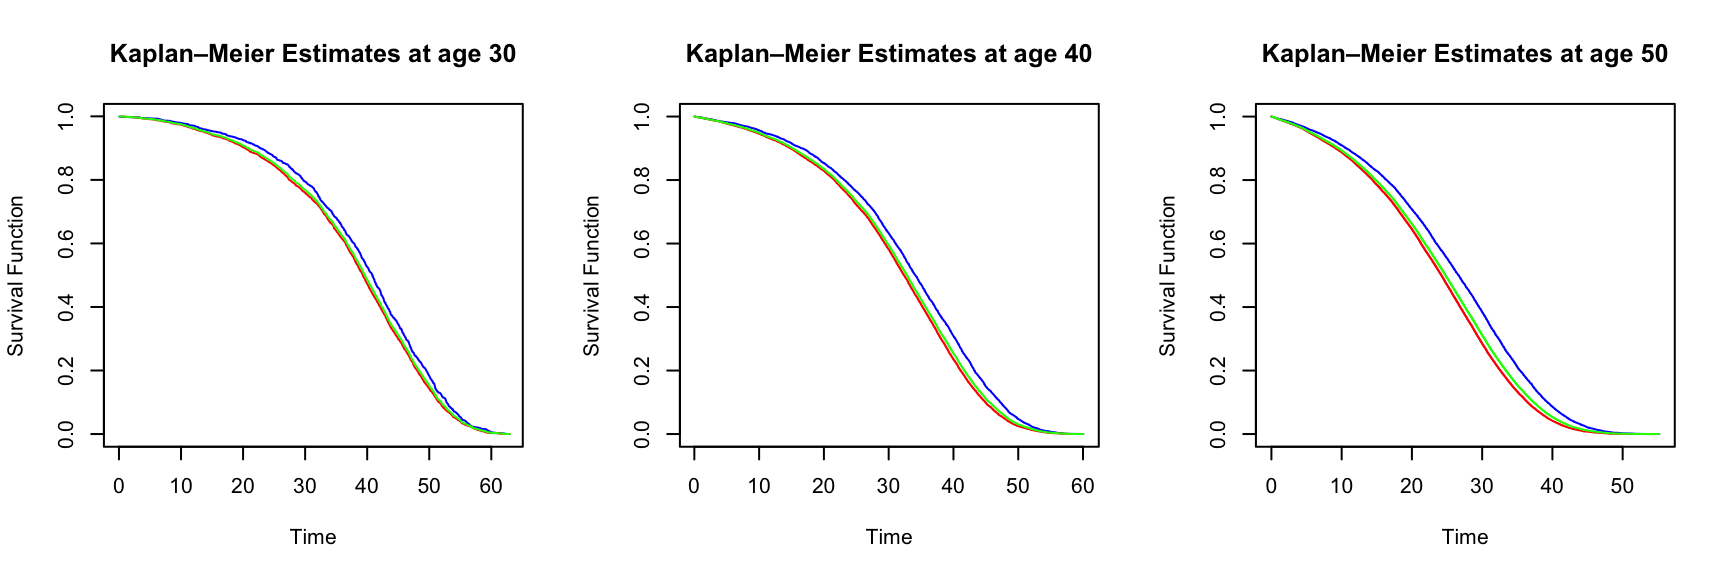
\includegraphics{LifeCon_files/figure-latex/KaplanMeierPlotsa-1} 

}

\caption{\textbf{Kaplan-Meier survival function estimates for an individual of age 30 (left), 40 (middle) and 50 (right) based on the insurer dataset -- curves are in blue (female), red (male) and green (all genders)}}\label{fig:KaplanMeierPlotsa}
\end{figure}

In line with results from the aggregate mortality data, Figure \ref{fig:KMFigs} tells us that females are more likely to survive over the same period than males. The curves for all genders are closer to the equivalent curves based on the male data, since the synthetic dataset has \(70\%\) male policyholders, as explained in the data summary given in Section \ref{S:IndivMortData}.

\hypertarget{nelson-aalen}{%
\subsection{Nelson-Aalen}\label{nelson-aalen}}

The Nelson-Aalen estimator provides a non-parametric estimat of the cumulative hazard rate function
\[
A_x(t) =\int_0^t \mu_x(s)\,ds.
\]
We have for the cumulative hazard rate:
\[
S_x(t+1) = \exp\{-A_x(t+1)\}=S_x(t)\,\exp\{-(A_x(t+1)-A_x(t))\}=S_x(t)\,\frac{l_{x+t+1}}{l_{x+t}}.
\]

To provide intuition for the Nelson-Aalen estimator, recall that for `small' arguments, the exponential function \(e^y \approx 1 + y\). Therefore, we have:
\[
1 - (A_x(t+1)-A_x(t)) \approx \frac{l_{x+t+1}}{l_{x+t}} \Longrightarrow A_x(t+1) \approx A_x(t) + \frac{d_{x+t}}{l_{x+t}}.
\]
However, in analogy to the derivation of the Kaplan-Meier estimat, the Nelson-Aalen estimator takes into account that in the context of right-censored individual mortality data, potential exposures at each death time may be different. That is, \(l_{x+t}\) in this equation should be interpreted as the total number of individuals at risk of dying at time \(x+t\). This number will change across time because individuals die \emph{and} because of right-censoring, so indviduals falling outside of the observation window. And, again, the estimator updates whenever there is a death event. The esimator thus amounts to nothing else than the sum of deaths over exposures. Again we refer to \href{https://openacttexts.github.io/Loss-Data-Analytics/C-ModelSelection.html\#nonparametric-estimation-using-modified-data}{Section 4.3.2 in Loss Data Analystics} for more information.

Using the library \texttt{survival}, we can also obtain Nelson-Aalen estimates of the survival curve. We estimate survival curves based on our insurer dataset from Section \ref{S:IndivMortData} for females and ages 30, 40, and 50.

R Code For Figure

\hypertarget{toggleCode.Nelson-Aalenux20Estimatesux20ofux20Survivalux20Curvesux20forux20agesux2030ux2cux2040ux2cux2050}{}
\begin{Shaded}
\begin{Highlighting}[]
\NormalTok{sexX <-}\StringTok{ }\DecValTok{0} \CommentTok{# 0 for female, 1 for male}
\CommentTok{# computations for individuals aged 50 }
\NormalTok{ageX <-}\StringTok{ }\DecValTok{50}
\NormalTok{setdata <-}\StringTok{ }\NormalTok{insdatatmp[}\KeywordTok{which}\NormalTok{(insdatatmp}\OperatorTok{$}\NormalTok{Age}\OperatorTok{+}\KeywordTok{floor}\NormalTok{(insdatatmp}\OperatorTok{$}\NormalTok{Time_of_death) }\OperatorTok{>=}\NormalTok{ageX }\OperatorTok{&}\StringTok{ }\NormalTok{insdatatmp}\OperatorTok{$}\NormalTok{Age }\OperatorTok{<=}\StringTok{ }\NormalTok{ageX }\OperatorTok{&}\StringTok{ }\NormalTok{insdatatmp}\OperatorTok{$}\NormalTok{Sex}\OperatorTok{==}\NormalTok{sexX),]}
\NormalTok{time <-}\StringTok{ }\KeywordTok{rep}\NormalTok{(}\DecValTok{0}\NormalTok{,}\KeywordTok{nrow}\NormalTok{(setdata))}
\NormalTok{status<-}\DecValTok{1}\OperatorTok{*}\NormalTok{(setdata}\OperatorTok{$}\NormalTok{Claim }\OperatorTok{==}\StringTok{ "YES"}\NormalTok{) }\CommentTok{# 0 for Censored data observations (i.e. with no claims and Claim=="No"), 1 for non-Censored observations -- setting for Survfit function}
\NormalTok{time <-}\StringTok{ }\NormalTok{setdata}\OperatorTok{$}\NormalTok{Time_of_death }\OperatorTok{-}\StringTok{ }\NormalTok{(}\KeywordTok{rep}\NormalTok{(ageX,}\KeywordTok{nrow}\NormalTok{(setdata))}\OperatorTok{-}\NormalTok{setdata}\OperatorTok{$}\NormalTok{Age)}
\NormalTok{fit_NA_}\DecValTok{50}\NormalTok{_F <-}\StringTok{ }\KeywordTok{survfit}\NormalTok{(}\KeywordTok{Surv}\NormalTok{(time,status) }\OperatorTok{~}\StringTok{ }\DecValTok{1}\NormalTok{, }\DataTypeTok{type=}\StringTok{'fleming-harrington'}\NormalTok{) }\CommentTok{# Nelson–Aalen estimator}

\CommentTok{# computations for individuals aged 40}
\NormalTok{ageX <-}\StringTok{ }\DecValTok{40}
\NormalTok{setdata <-}\StringTok{ }\NormalTok{insdatatmp[}\KeywordTok{which}\NormalTok{(insdatatmp}\OperatorTok{$}\NormalTok{Age}\OperatorTok{+}\KeywordTok{floor}\NormalTok{(insdatatmp}\OperatorTok{$}\NormalTok{Time_of_death) }\OperatorTok{>=}\NormalTok{ageX }\OperatorTok{&}\StringTok{ }\NormalTok{insdatatmp}\OperatorTok{$}\NormalTok{Age }\OperatorTok{<=}\StringTok{ }\NormalTok{ageX }\OperatorTok{&}\StringTok{ }\NormalTok{insdatatmp}\OperatorTok{$}\NormalTok{Sex}\OperatorTok{==}\NormalTok{sexX),]}
\NormalTok{time <-}\StringTok{ }\KeywordTok{rep}\NormalTok{(}\DecValTok{0}\NormalTok{,}\KeywordTok{nrow}\NormalTok{(setdata))}
\NormalTok{status<-}\DecValTok{1}\OperatorTok{*}\NormalTok{(setdata}\OperatorTok{$}\NormalTok{Claim }\OperatorTok{==}\StringTok{ "YES"}\NormalTok{) }\CommentTok{# 0 for Censored data observations (i.e. with no claims and Claim=="No"), 1 for non-Censored observations -- setting for Survfit function}
\NormalTok{time <-}\StringTok{ }\NormalTok{setdata}\OperatorTok{$}\NormalTok{Time_of_death }\OperatorTok{-}\StringTok{ }\NormalTok{(}\KeywordTok{rep}\NormalTok{(ageX,}\KeywordTok{nrow}\NormalTok{(setdata))}\OperatorTok{-}\NormalTok{setdata}\OperatorTok{$}\NormalTok{Age)}
\NormalTok{fit_NA_}\DecValTok{40}\NormalTok{_F <-}\StringTok{ }\KeywordTok{survfit}\NormalTok{(}\KeywordTok{Surv}\NormalTok{(time,status) }\OperatorTok{~}\StringTok{ }\DecValTok{1}\NormalTok{, }\DataTypeTok{type=}\StringTok{'fleming-harrington'}\NormalTok{) }\CommentTok{# Nelson–Aalen estimator}

\CommentTok{# computations for individuals aged 30}
\NormalTok{ageX <-}\StringTok{ }\DecValTok{30}
\NormalTok{setdata <-}\StringTok{ }\NormalTok{insdatatmp[}\KeywordTok{which}\NormalTok{(insdatatmp}\OperatorTok{$}\NormalTok{Age}\OperatorTok{+}\KeywordTok{floor}\NormalTok{(insdatatmp}\OperatorTok{$}\NormalTok{Time_of_death) }\OperatorTok{>=}\NormalTok{ageX }\OperatorTok{&}\StringTok{ }\NormalTok{insdatatmp}\OperatorTok{$}\NormalTok{Age }\OperatorTok{<=}\StringTok{ }\NormalTok{ageX }\OperatorTok{&}\StringTok{ }\NormalTok{insdatatmp}\OperatorTok{$}\NormalTok{Sex}\OperatorTok{==}\NormalTok{sexX),]}
\NormalTok{time <-}\StringTok{ }\KeywordTok{rep}\NormalTok{(}\DecValTok{0}\NormalTok{,}\KeywordTok{nrow}\NormalTok{(setdata))}
\NormalTok{status<-}\DecValTok{1}\OperatorTok{*}\NormalTok{(setdata}\OperatorTok{$}\NormalTok{Claim }\OperatorTok{==}\StringTok{ "YES"}\NormalTok{) }\CommentTok{# 0 for Censored data observations (i.e. with no claims and Claim=="No"), 1 for non-Censored observations -- setting for Survfit function}
\NormalTok{time <-}\StringTok{ }\NormalTok{setdata}\OperatorTok{$}\NormalTok{Time_of_death }\OperatorTok{-}\StringTok{ }\NormalTok{(}\KeywordTok{rep}\NormalTok{(ageX,}\KeywordTok{nrow}\NormalTok{(setdata))}\OperatorTok{-}\NormalTok{setdata}\OperatorTok{$}\NormalTok{Age)}
\NormalTok{fit_NA_}\DecValTok{30}\NormalTok{_F <-}\StringTok{ }\KeywordTok{survfit}\NormalTok{(}\KeywordTok{Surv}\NormalTok{(time,status) }\OperatorTok{~}\StringTok{ }\DecValTok{1}\NormalTok{, }\DataTypeTok{type=}\StringTok{'fleming-harrington'}\NormalTok{) }\CommentTok{# Nelson–Aalen estimator}

\CommentTok{# survival function plots}
\KeywordTok{par}\NormalTok{(}\DataTypeTok{mfrow=}\KeywordTok{c}\NormalTok{(}\DecValTok{1}\NormalTok{,}\DecValTok{3}\NormalTok{))}
\KeywordTok{plot}\NormalTok{(fit_NA_}\DecValTok{30}\NormalTok{_F}\OperatorTok{$}\NormalTok{surv}\OperatorTok{~}\NormalTok{fit_NA_}\DecValTok{30}\NormalTok{_F}\OperatorTok{$}\NormalTok{time,}\DataTypeTok{type=}\StringTok{"l"}\NormalTok{, }\DataTypeTok{main=}\StringTok{"Nelson-Aalen Estimates at age 30"}\NormalTok{, }\DataTypeTok{xlab=}\StringTok{"Time"}\NormalTok{, }\DataTypeTok{ylab=}\StringTok{"Survival Function"}\NormalTok{,}\DataTypeTok{col =} \StringTok{"blue"}\NormalTok{)}
\KeywordTok{plot}\NormalTok{(fit_NA_}\DecValTok{40}\NormalTok{_F}\OperatorTok{$}\NormalTok{surv}\OperatorTok{~}\NormalTok{fit_NA_}\DecValTok{40}\NormalTok{_F}\OperatorTok{$}\NormalTok{time,}\DataTypeTok{type=}\StringTok{"l"}\NormalTok{, }\DataTypeTok{main=}\StringTok{"Nelson-Aalen Estimates at age 40"}\NormalTok{, }\DataTypeTok{xlab=}\StringTok{"Time"}\NormalTok{, }\DataTypeTok{ylab=}\StringTok{"Survival Function"}\NormalTok{,}\DataTypeTok{col =} \StringTok{"blue"}\NormalTok{)}
\KeywordTok{plot}\NormalTok{(fit_NA_}\DecValTok{50}\NormalTok{_F}\OperatorTok{$}\NormalTok{surv}\OperatorTok{~}\NormalTok{fit_NA_}\DecValTok{50}\NormalTok{_F}\OperatorTok{$}\NormalTok{time,}\DataTypeTok{type=}\StringTok{"l"}\NormalTok{, }\DataTypeTok{main=}\StringTok{"Nelson-Aalen Estimates at age 50"}\NormalTok{, }\DataTypeTok{xlab=}\StringTok{"Time"}\NormalTok{, }\DataTypeTok{ylab=}\StringTok{"Survival Function"}\NormalTok{,}\DataTypeTok{col =} \StringTok{"blue"}\NormalTok{)}
\end{Highlighting}
\end{Shaded}



\begin{figure}

{\centering 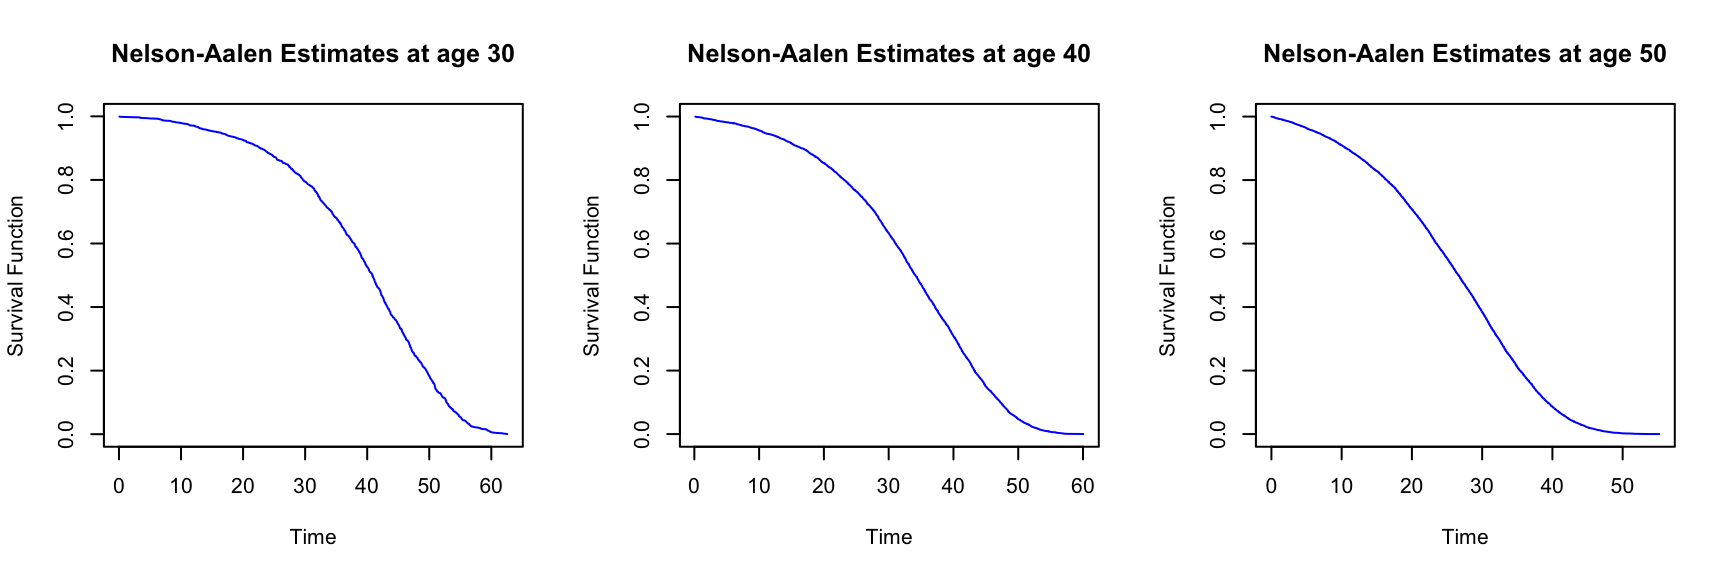
\includegraphics{LifeCon_files/figure-latex/NelsonAalenPlotsa-1} 

}

\caption{\textbf{Nelson-Aalen survival function estimates for females of age 30 (left), 40 (middle) and 50 (right) based on the insurer dataset}}\label{fig:NelsonAalenPlotsa}
\end{figure}

Given that the dataset has a large sample size, the differences between the \emph{Kaplan-Meier} and \emph{Nelson-Aalen} estimates are insignificant; this is not surprising, since the two estimators are asymptotically equivalent -- for large samples, the estimators are supposed to provide the same results.

Since the \emph{Kaplan-Meier} and \emph{Nelson-Aalen} estimators provide a full non-parametric estimate of the survival curve, we can directly use it for evaluating quantities depending on the distribution of the lifetime random variable. In principle, there is no need to discretize it to compile a life table -- although that's certainly possible. To reiterate, the approach in the application is to assemble a suitable set of lives and determine a survival function viewing these lives as a (sufficiently) homogeneous population. In the next section, we consider survival analysis models that explicitly account for the heterogeneity of individuals' exposures by accounting for their characteristics.

\hypertarget{S:SurvReg}{%
\section{Conditional models: Survival regression}\label{S:SurvReg}}

All models introduced in the foregoing sections \ref{S:AnalMortLaws} (analytic mortality laws), \ref{S:LifeTab} (life tables based on mortality count data), and \ref{S:NonParamSurv} (non-parametric estimates of the survival curve based on a homogeneous population) are based on the age-only model that -- with some qualifications (see, e.g., Section \ref{S:LifeTabMImpr}). However, as introduced in Section \ref{S:IndivMortData}, individual \emph{survival} or \emph{event} data that an insurance company has available consists of \emph{features} or \emph{covariates} \({\bf{x}}_i\) for each individual \(i\), plus the death time \(T_i\) if the individual had died or -- if that's not the case -- the information that the individual is still alive. Hence, a proximate approach is to directly model the individual lifetime distribution \(T_{{\bf{x}}_i}\), i.e., to explicitly account for the heterogeneity in the individuals' exposures. This can be accomplished via so-called \emph{survival regression} models that predict the distribution of \(T_{{\bf{x}}}\) based on a set of features \({\bf{x}}_i\) and death times \(T_i\), \(i=1,2,\cdots,N\).

Our objective is to introduce some key ideas and to derive workable models. Therefore, we primarily focus on the most popular model -- namely the proportional hazard (Cox) model -- and consider linear models in the features. A detailed introduction of this rich set of models is beyond the scope of this text, although we note that in principle more sophisticated models can be used. We refer to the Notes and Comments section at the end of this chapter for references that go beyond our introduction.

We start by introducing the Cox proportional hazard model in the first part. We apply it to our individual level mortality dataset from Section \ref{S:IndivMortData} in the second part. And, finally, we show how to produce different models and life tables on the basis of the regression model.

\hypertarget{the-cox-proportional-hazard-model}{%
\subsection{The Cox Proportional Hazard Model}\label{the-cox-proportional-hazard-model}}

The task at hand is to formulate a model for the \emph{individual} survival function \(S_{\bf{x}}(\cdot)\) given a feature vector \(\bf{x}\). Concretely, this may mean specifying a parametric model, i.e., to posit that \(S_{\bf{x}}(t)\) takes a certain functional form of time \(t\), the features \(\bf{x}\), and certain parameters, say \(\beta\). We can then try to estimate the parameters based on our data \(({\bf{x}}_i,T_i)_{1\leq i \leq N}\). However, a key challenge are the boundedness and monotonicity constraints for the survival function \(S_{\bf{x}}(\cdot)\).

Therefore, it is common in survival analysis to model the \emph{individual} force of mortality (or hazard function) \(\mu_{\bf{x}}(\cdot)\). In principle, \(\mu_{\bf{x}}(t)\) can take any positive number, although as we had discussed in Section @ref\{S:AnalMortLaws\} a human's force of mortality typically increases in age. Hence, a common approach in survival analysis is to posit that \(\mu_{\bf{x}}(t)\) takes a certain functional form of time \(t\), the features \(\bf{x}\), and parameters \(\beta\), and then try to estimate the parameters based on our data \(({\bf{x}}_i,T_i)_{1\leq i \leq N}\).

Different functional forms are possible. For example, additive survvial regression models specify \(\mu_{\bf{x}}(t)\) as a linear combination of the features, similarly to linear regression models. However, the most popular approach -- due to its tractability and fit in many situations -- is the so-called \emph{Cox proportional hazard model}. In its simplest form, it assumes the force of mortality takes the form:
\[
\mu_{\bf{x}}(t)=\beta_0(t) \times \exp\left\{ \beta' \,{\bf{x}}\right\},
\]
in which \(\beta\) is the vector of regression parameters. The non-parametric term \(\beta_0(t)\) is also referred to as the \textit{nuisance} parameter when the emphasis is on the estimation of the regression coefficients. It is also possible to allow for time-varying covariates:
\[
\mu_{\bf{x}}(t) = \beta_0(t)\times\exp\left\{\beta'\, {\bf{x}}(t)\right\},
\]
where \({\bf{x}}(t)\) are (possibly) time-varying covariates. Since the covariates are given, we in order to obtain (an estimate for) \(\mu_{\bf{x}}(t)\), we need to estimate the parameter vector \(\beta\). We outline the estimation process below, although the details are not crucial for the material that follows.

Estimation of the Regression Parameters in the Proportional Hazards Model

\leavevmode\hypertarget{toggleTheory.EstimationCoxModel}{}%
For a set of \(N\) independent subjects, define the observation time \(X_i = \min\{T_i, C_i\}\), \(i\in\{1,\ldots,n\}\), where \(T_i\) is time until death and \(C_i\) is the censoring time (time until end of observation period) for subject \(i\). The indicator for observed death of subject \(i\) is defined as \(\Delta_i = 1_{\{T_i < C_i\}}\). We further define the \(i\)-th at-risk and observed-death counting processes as \(Y_i(t)=1_{\{X_i\ge t\}}\) and \(N_i(t)=1_{\{T_i\le t,\Delta_i=1\}}\), respectively.

The likelihood-based estimation relies on a similar idea as the Nelson-Aalen estimator from Section \ref{S:NonParamSurv}: We determine parameters such that the observed death of individual \(i\) at time \(T_i\) is most likely amount all possible death. More precisely, the likelihood for individual \(i\) is
\[
L_i(\beta) = \frac{\mu_{\bf{x_i}}(T_i)}{\sum_{j=1}^N Y_j(T_i)\,\mu_{\bf{x_j}}(T_i)}=\frac{\exp\left\{\beta'\, {\bf{x}_i}(T_i)\right\}}{\sum_{j=1}^N Y_j(T_i)\,\exp\left\{\beta'\, {\bf{x}}_j(T_i)\right\}},
\]
and the total likelihood \(L(\beta) = \prod_i L_i(\beta)\). The partial log-likelihood function can then be expressed as:
\[
l(\beta) = \sum_{i=1}^N \Delta_i\left\{\beta'\, {\bf{x}}_i(T_i) - \ln\left(\sum_{j=1}^n Y_j(T_i)\exp\left\{\beta'\, {\bf{x}}_j(T_i)\right\} \right)  \right\}.
\]
Differentiating yields the (partial-likelihood) score function:
\begin{eqnarray*}
U(\beta) = \frac{\partial l(\beta)}{\partial \beta} & = & \sum_{i=1}^N \Delta_i\Bigg\{ {\bf{x}}_i(T_i) - \underbrace{\frac{\sum_{j=1}^N Y_j(T_i)\,{\bf{x}}_j(T_i)\exp\{\beta'\, {\bf{x}}_j(T_i)\}}{\sum_{j=1}^n Y_j(T_i)\exp\{\beta'\, {\bf{x}}_j(T_i)\}}}_{\bar{Z}(T_i)}  \Bigg\} \\
& = & \sum_{i=1}^n \int_0^{\infty} \left[ {\bf{x}}_i(t) - \bar{Z}(t) \right] dN_i(t).
\end{eqnarray*}
The parameter vector is then estimated as the solution to the score equation \(U(\beta)=0\), without estimating the nuisance parameter \(\beta_0(t)\).

\hypertarget{cox-models-based-on-life-insurer-data}{%
\subsection{Cox Models Based on Life Insurer Data}\label{cox-models-based-on-life-insurer-data}}

We estimate proportional hazard models based on our dataset from Section \ref{S:IndivMortData}. We start with a simple model that only includes age and sex:
\[
\mu_{(x_0,s)}(t) = \beta_0(t)\,\exp\{\beta_{\text{age}}(x_0+t)+\beta_{\text{male}}\,1_{\{s=\text{male}\}}\}=\underbrace{\beta_0(t)\,e^{\beta_{\text{age}}\,t}}_{\tilde{\beta}_0(t)}\,\exp\{\beta_{\text{age}}\,x_0+\beta_{\text{male}}\,1_{\{s=\text{male}\}}\}.
\]
In particular, since age enters the equation linearly, although age varies with time, the time variation will be absorbed in the nuisance parameter \(\tilde{\beta}_0(t)\) so we don't have to account for the time-varying nature of age.

Running the model is straightforward relying on the library \texttt{survival}, where we only have to assure that we label the censored vs.~non-censored event times appropriately:

\begin{Shaded}
\begin{Highlighting}[]
\NormalTok{ins_data <-}\StringTok{ }\KeywordTok{fread}\NormalTok{(}\StringTok{"Data/SyntheticInsurerData.csv"}\NormalTok{,}\DataTypeTok{data.table=}\OtherTok{FALSE}\NormalTok{)}
\KeywordTok{library}\NormalTok{(survival)}
\NormalTok{CensorTime <-}\StringTok{ }\NormalTok{(}\DecValTok{781}\OperatorTok{-}\NormalTok{ins_data}\OperatorTok{$}\NormalTok{Month_of_Sale)}\OperatorTok{/}\DecValTok{12}
\NormalTok{ins_data}\OperatorTok{$}\NormalTok{EventTime <-}\StringTok{ }\KeywordTok{rep}\NormalTok{(}\DecValTok{0}\NormalTok{,}\DecValTok{160781}\NormalTok{)}
\NormalTok{ins_data}\OperatorTok{$}\NormalTok{EventTime[}\KeywordTok{is.na}\NormalTok{(ins_data}\OperatorTok{$}\NormalTok{Time_of_death)] <-}\StringTok{ }\NormalTok{CensorTime[}\KeywordTok{is.na}\NormalTok{(ins_data}\OperatorTok{$}\NormalTok{Time_of_death)]}
\NormalTok{ins_data}\OperatorTok{$}\NormalTok{EventTime[}\OperatorTok{!}\KeywordTok{is.na}\NormalTok{(ins_data}\OperatorTok{$}\NormalTok{Time_of_death)] <-}\StringTok{ }\NormalTok{ins_data}\OperatorTok{$}\NormalTok{Time_of_death[}\OperatorTok{!}\KeywordTok{is.na}\NormalTok{(ins_data}\OperatorTok{$}\NormalTok{Time_of_death)]}
\NormalTok{ins_data}\OperatorTok{$}\NormalTok{Claim <-}\StringTok{ }\DecValTok{1}\OperatorTok{*}\NormalTok{(ins_data}\OperatorTok{$}\NormalTok{Claim }\OperatorTok{==}\StringTok{ "YES"}\NormalTok{)}

\NormalTok{Cox_ph_}\DecValTok{1}\NormalTok{ <-}\StringTok{ }\KeywordTok{coxph}\NormalTok{(}\KeywordTok{Surv}\NormalTok{(EventTime, Claim) }\OperatorTok{~}\StringTok{ }\NormalTok{Age }\OperatorTok{+}\StringTok{ }\NormalTok{Sex, }\DataTypeTok{data=}\NormalTok{ins_data)}
\KeywordTok{summary}\NormalTok{(Cox_ph_}\DecValTok{1}\NormalTok{)}
\end{Highlighting}
\end{Shaded}

\begin{verbatim}
Call:
coxph(formula = Surv(EventTime, Claim) ~ Age + Sex, data = ins_data)

  n= 160781, number of events= 59382 

           coef   exp(coef)    se(coef)       z   Pr(>|z|)    
Age 0.117981709 1.125223530 0.000469934 251.060 < 2.22e-16 ***
Sex 0.390607312 1.477878055 0.009256317  42.199 < 2.22e-16 ***
---
Signif. codes:  0 '***' 0.001 '**' 0.01 '*' 0.05 '.' 0.1 ' ' 1

    exp(coef) exp(-coef) lower .95 upper .95
Age   1.12522   0.888712   1.12419   1.12626
Sex   1.47788   0.676646   1.45131   1.50493

Concordance= 0.812  (se = 0.001 )
Likelihood ratio test= 71813.2  on 2 df,   p=<2e-16
Wald test            = 63529.2  on 2 df,   p=<2e-16
Score (logrank) test = 72775.3  on 2 df,   p=<2e-16
\end{verbatim}

We obtain positive coefficients for age and sex. Indeed, the coefficient is similar -- though slightly larger -- than the Gompertz coefficients \(c\) in Section \ref{S:AnalMortLaws}. Note that this does not mean that mortality rates for this insured poulation, it just means that the increase in age is steeper. Indeed, a steeper, ``hockey-stick'' shaped mortality curve associated with a compression of mortality -- sometimes referred to as \emph{rectangularization} -- for certain populations with higher life expectancies is not uncommon. We also observe a positive sign for the \emph{Male} coefficient implying higher mortality for males, compared to females of the same age.

The key advantage of the proportional hazard model is that we can take into account all features. A model building process may contemplate the (statistical) significance of the different covariates. We may also probe whether a linear model is appropriate for the different features, or whether their influence is better captured via non-linear relationships. Furthermore, we may analyze whether interactions of the features are relevant. Different models can be compared based on the \emph{Akaike information criterion} (AIC), where the objective is to determine a model with a low AIC:

\begin{Shaded}
\begin{Highlighting}[]
\KeywordTok{extractAIC}\NormalTok{(Cox_ph_}\DecValTok{1}\NormalTok{)}
\end{Highlighting}
\end{Shaded}

\begin{verbatim}
[1]       2.00 1220422.68
\end{verbatim}

We leave the exploration of different models to the interested reader, and cut immediately to the model that performs best. This model includes all features, but no interaction or non-linear terms. In analogy to the simple model above, age and potential time (\(t\)) effects are absorbed in the nuisance term, so that we do not have to explicitly account for time-varying covariates.

Again, we run the model relying on the library \texttt{survival}:

\begin{Shaded}
\begin{Highlighting}[]
\NormalTok{Cox_ph_}\DecValTok{2}\NormalTok{ <-}\StringTok{ }\KeywordTok{coxph}\NormalTok{(}\KeywordTok{Surv}\NormalTok{(EventTime, Claim) }\OperatorTok{~}\StringTok{ }\NormalTok{Month_of_Sale }\OperatorTok{+}\StringTok{ }\NormalTok{Age }\OperatorTok{+}\StringTok{ }\NormalTok{Sex  }\OperatorTok{+}\StringTok{ }\NormalTok{BloodPressure }\OperatorTok{+}
\StringTok{                  }\NormalTok{Smoking }\OperatorTok{+}\StringTok{ }\NormalTok{(BMI}\OperatorTok{>}\DecValTok{30}\NormalTok{) , }\DataTypeTok{data=}\NormalTok{ins_data)}
\KeywordTok{summary}\NormalTok{(Cox_ph_}\DecValTok{2}\NormalTok{)}
\end{Highlighting}
\end{Shaded}

\begin{verbatim}
Call:
coxph(formula = Surv(EventTime, Claim) ~ Month_of_Sale + Age + 
    Sex + BloodPressure + Smoking + (BMI > 30), data = ins_data)

  n= 160781, number of events= 59382 

                       coef     exp(coef)      se(coef)        z   Pr(>|z|)    
Month_of_Sale -0.0010889204  0.9989116723  0.0000327369 -33.2628 < 2.22e-16 ***
Age            0.1178051484  1.1250248771  0.0005214675 225.9108 < 2.22e-16 ***
Sex            0.3991615411  1.4905743882  0.0092796785  43.0146 < 2.22e-16 ***
BloodPressure  0.0162349216  1.0163674240  0.0003058399  53.0831 < 2.22e-16 ***
Smoking        0.7832951724  2.1886724491  0.0085781538  91.3128 < 2.22e-16 ***
BMI > 30TRUE   0.2736998514  1.3148201015  0.0149480591  18.3101 < 2.22e-16 ***
---
Signif. codes:  0 '***' 0.001 '**' 0.01 '*' 0.05 '.' 0.1 ' ' 1

              exp(coef) exp(-coef) lower .95 upper .95
Month_of_Sale  0.998912   1.001090  0.998848  0.998976
Age            1.125025   0.888869  1.123876  1.126175
Sex            1.490574   0.670882  1.463709  1.517933
BloodPressure  1.016367   0.983896  1.015758  1.016977
Smoking        2.188672   0.456898  2.152182  2.225781
BMI > 30TRUE   1.314820   0.760560  1.276858  1.353911

Concordance= 0.828  (se = 0.001 )
Likelihood ratio test= 84426.5  on 6 df,   p=<2e-16
Wald test            = 71241.8  on 6 df,   p=<2e-16
Score (logrank) test = 82479.9  on 6 df,   p=<2e-16
\end{verbatim}

We observe that all variables are highly significant. The coefficients for age and sex are similar as in the simpler model above. Similarly, high blood pressure, smoking, and a higher blood pressure lead to a higher mortality, whereas later sales are associated with a lower mortality. The latter amounts to a negative trend in mortality, or in other words increasing longevity over time.

As a key application, we can now produce survival curves for a given set of covariates. We consider survival curves for age 75 and different genders and smoking status, and survival curves for for 60-year old feamess with different BMI and blood pressure levels. We consider all of these at the last month of sales in our dataset.

R Code For Figure

\hypertarget{toggleCode.Survivalux20Curvesux20basedux20onux20theux20Coxux20Model}{}
\begin{Shaded}
\begin{Highlighting}[]
\KeywordTok{par}\NormalTok{(}\DataTypeTok{mfrow=}\KeywordTok{c}\NormalTok{(}\DecValTok{1}\NormalTok{,}\DecValTok{2}\NormalTok{))}
\NormalTok{Survfunction <-}\StringTok{ }\ControlFlowTok{function}\NormalTok{(Month_of_Sale, Age, }\DataTypeTok{Sex=}\DecValTok{0}\NormalTok{, }\DataTypeTok{Smoking=}\DecValTok{0}\NormalTok{, }\DataTypeTok{BMI=}\DecValTok{25}\NormalTok{, }\DataTypeTok{BloodPressure=}\DecValTok{120}\NormalTok{)\{}
\NormalTok{  Claim <-}\StringTok{ }\DecValTok{0}
\NormalTok{  EventTime <-}\StringTok{ }\DecValTok{1}
\NormalTok{  sfun <-}\StringTok{ }\KeywordTok{survfit}\NormalTok{(Cox_ph_}\DecValTok{2}\NormalTok{,}\DataTypeTok{newdata =} \KeywordTok{data.frame}\NormalTok{(Month_of_Sale,Age,Sex,Smoking,BMI,BloodPressure,Claim,EventTime))}
\NormalTok{\}}

\NormalTok{s <-}\StringTok{ }\KeywordTok{Survfunction}\NormalTok{(}\DecValTok{780}\NormalTok{,}\DecValTok{75}\NormalTok{)}
\NormalTok{s2 <-}\StringTok{ }\KeywordTok{Survfunction}\NormalTok{(}\DecValTok{780}\NormalTok{,}\DecValTok{75}\NormalTok{, }\DataTypeTok{Smoking=}\DecValTok{1}\NormalTok{)}
\NormalTok{s3 <-}\StringTok{ }\KeywordTok{Survfunction}\NormalTok{(}\DecValTok{780}\NormalTok{,}\DecValTok{75}\NormalTok{, }\DataTypeTok{Sex =} \DecValTok{1}\NormalTok{)}
\NormalTok{s4 <-}\StringTok{ }\KeywordTok{Survfunction}\NormalTok{(}\DecValTok{780}\NormalTok{,}\DecValTok{75}\NormalTok{, }\DataTypeTok{Sex =} \DecValTok{1}\NormalTok{, }\DataTypeTok{Smoking=}\DecValTok{1}\NormalTok{)}
\KeywordTok{plot}\NormalTok{(s,}\DataTypeTok{col=}\StringTok{"orange"}\NormalTok{,}\DataTypeTok{main=}\StringTok{"Suvival functions for 75-year olds"}\NormalTok{, }\DataTypeTok{xlab=}\StringTok{"Time"}\NormalTok{, }\DataTypeTok{ylab=}\StringTok{"Survival Function"}\NormalTok{)}
\KeywordTok{lines}\NormalTok{(s2,}\DataTypeTok{col=}\StringTok{"red"}\NormalTok{)}
\KeywordTok{lines}\NormalTok{(s3, }\DataTypeTok{col =} \StringTok{"green"}\NormalTok{)}
\KeywordTok{lines}\NormalTok{(s4, }\DataTypeTok{col =} \StringTok{"blue"}\NormalTok{)}

\NormalTok{s <-}\StringTok{ }\KeywordTok{Survfunction}\NormalTok{(}\DecValTok{780}\NormalTok{,}\DecValTok{60}\NormalTok{)}
\NormalTok{s2 <-}\StringTok{ }\KeywordTok{Survfunction}\NormalTok{(}\DecValTok{780}\NormalTok{,}\DecValTok{60}\NormalTok{, }\DataTypeTok{BMI =} \DecValTok{30}\NormalTok{, }\DataTypeTok{BloodPressure =} \DecValTok{140}\NormalTok{)}
\NormalTok{s3 <-}\StringTok{ }\KeywordTok{Survfunction}\NormalTok{(}\DecValTok{780}\NormalTok{,}\DecValTok{60}\NormalTok{, }\DataTypeTok{BMI =} \DecValTok{35}\NormalTok{, }\DataTypeTok{BloodPressure =} \DecValTok{160}\NormalTok{)}
\NormalTok{s4 <-}\StringTok{ }\KeywordTok{Survfunction}\NormalTok{(}\DecValTok{780}\NormalTok{,}\DecValTok{60}\NormalTok{, }\DataTypeTok{BMI =} \DecValTok{40}\NormalTok{, }\DataTypeTok{BloodPressure =} \DecValTok{180}\NormalTok{)}
\KeywordTok{plot}\NormalTok{(s,}\DataTypeTok{col=}\StringTok{"orange"}\NormalTok{,}\DataTypeTok{main=}\StringTok{"Suvival functions for 60-year olds"}\NormalTok{, }\DataTypeTok{xlab=}\StringTok{"Time"}\NormalTok{, }\DataTypeTok{ylab=}\StringTok{"Survival Function"}\NormalTok{)}
\KeywordTok{lines}\NormalTok{(s2,}\DataTypeTok{col=}\StringTok{"red"}\NormalTok{)}
\KeywordTok{lines}\NormalTok{(s3, }\DataTypeTok{col =} \StringTok{"green"}\NormalTok{)}
\KeywordTok{lines}\NormalTok{(s4, }\DataTypeTok{col =} \StringTok{"blue"}\NormalTok{)}
\end{Highlighting}
\end{Shaded}



\begin{figure}

{\centering 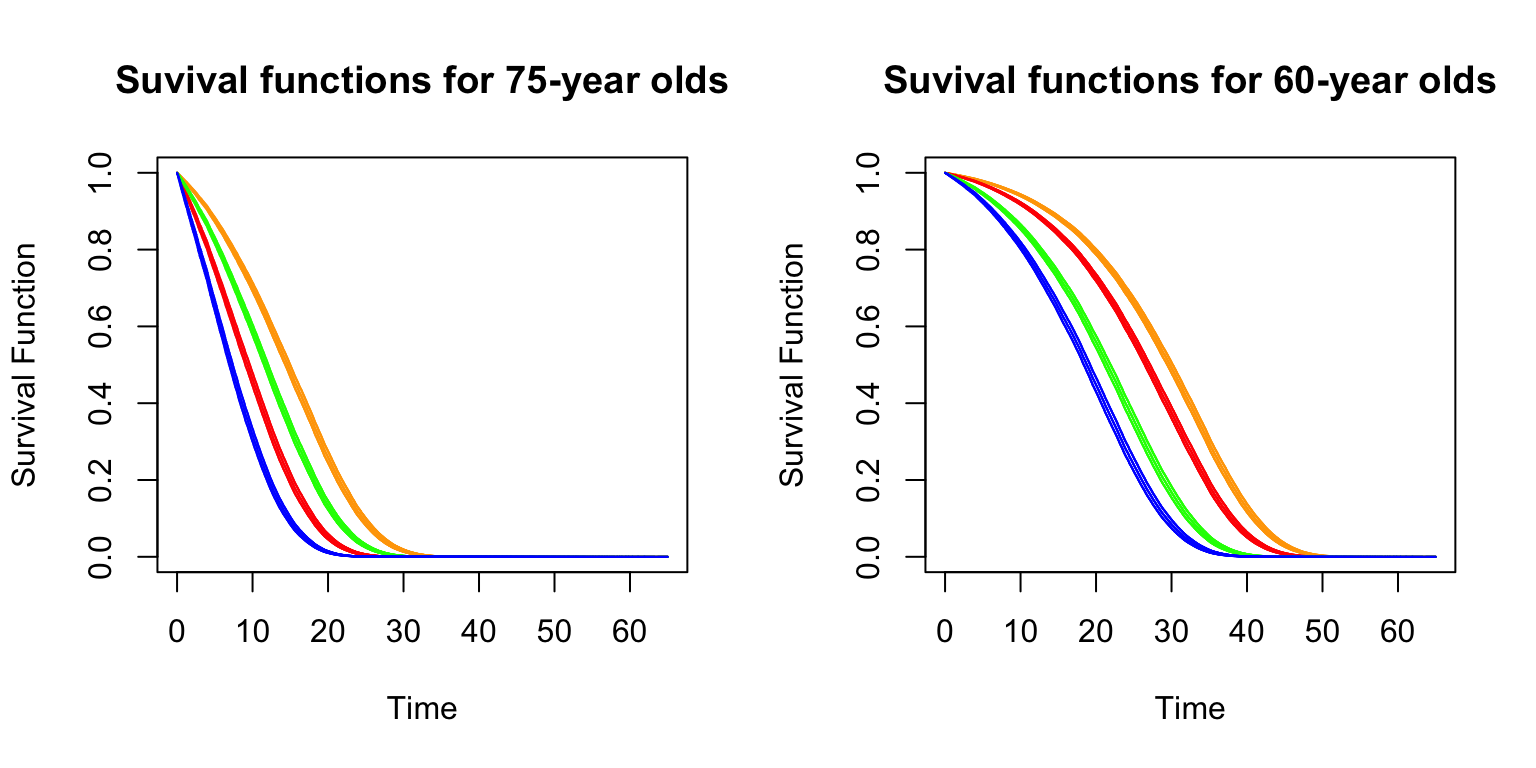
\includegraphics{LifeCon_files/figure-latex/CoxPHPlotsa-1} 

}

\caption{\textbf{Survival functions for age 75 and different genders and smoking status (left), and survival curves for for 60-year old feamess with different BMI and blood pressure levels (right)}}\label{fig:CoxPHPlotsa}
\end{figure}

The survival functions are shown including 95\% confidence intervals. As is evident, the covariates substantially affect the survival functions. Indeed, while 75-year old females have better survival prospects than males (orange vs.~green curve on the left-hand side), female smokers are worse off than male non-smokers (green vs.~red curve on the left-hand side) -- while male smokers have the bleakest survival prospects (blue curve on the left-hand side). Similarly, for the 60-year old females, individuals with the low BMI and low blood pressure with a median future lifetime of more than 30 years (orange curve on the right-hand side), whereas for the highest levels of BMI (40) and systolic blood pressure (180), the median future lifetime is less than 20 years (blue curve on the right-hand side). We notice the inframarginal decrease in the survival probabilities as the BMI exceeds 30.

\hypertarget{conditional-life-tables}{%
\subsection{Conditional Life Tables}\label{conditional-life-tables}}

Recall that a life table is a discretized version of the survival function. Therefore, we can rely on the estimated survival function to generate a life table. We consider the example of a newly underwritten life in the month after the end of our dataset, for a 42-year-old non-smoking male with a BMI of 28 and a blood pressure of 127. We consider the discretized version of the survival function and determine annualized mortality probabilities \(q_{x+t}\), according to the formulas provides in Section \ref{Sec:ModelingDeaths}.

R Code For Figure

\hypertarget{toggleCode.Mortalityux20Probabilitiesux20forux20aux2042-year-oldux20male}{}
\begin{Shaded}
\begin{Highlighting}[]
\KeywordTok{par}\NormalTok{(}\DataTypeTok{mfrow=}\KeywordTok{c}\NormalTok{(}\DecValTok{1}\NormalTok{,}\DecValTok{1}\NormalTok{))}
\NormalTok{s <-}\StringTok{ }\KeywordTok{Survfunction}\NormalTok{(}\DecValTok{781}\NormalTok{,}\DecValTok{42}\NormalTok{,}\DecValTok{1}\NormalTok{,}\DecValTok{0}\NormalTok{,}\DecValTok{28}\NormalTok{,}\DecValTok{127}\NormalTok{)}
\NormalTok{S_x_t <-}\StringTok{ }\KeywordTok{summary}\NormalTok{(s,}\DataTypeTok{times =} \DecValTok{0}\OperatorTok{:}\DecValTok{68}\NormalTok{)}\OperatorTok{$}\NormalTok{surv}
\NormalTok{q_x_t <-}\StringTok{ }\KeywordTok{rep}\NormalTok{(}\DecValTok{0}\NormalTok{,}\DecValTok{64}\NormalTok{)}
\ControlFlowTok{for}\NormalTok{(i }\ControlFlowTok{in} \DecValTok{1}\OperatorTok{:}\DecValTok{64}\NormalTok{)\{}
\NormalTok{  q_x_t[i] <-}\StringTok{ }\NormalTok{(S_x_t[i] }\OperatorTok{-}\StringTok{ }\NormalTok{S_x_t[i}\OperatorTok{+}\DecValTok{1}\NormalTok{])}\OperatorTok{/}\NormalTok{S_x_t[i] }
\NormalTok{\}}
\KeywordTok{plot}\NormalTok{(q_x_t,}\DataTypeTok{main=}\StringTok{"Mortality probabilities for 42 + t"}\NormalTok{, }\DataTypeTok{xlab=}\StringTok{"t"}\NormalTok{, }\DataTypeTok{ylab=}\StringTok{"q_x+t"}\NormalTok{)}
\KeywordTok{lines}\NormalTok{(q_x_t, }\DataTypeTok{lwd =} \DecValTok{2}\NormalTok{, }\DataTypeTok{col =} \StringTok{"blue"}\NormalTok{)}
\NormalTok{xs <-}\StringTok{ }\DecValTok{1}\OperatorTok{:}\DecValTok{64}
\NormalTok{q_x_t_smoothed <-}\StringTok{ }\KeywordTok{predict}\NormalTok{(}\KeywordTok{loess}\NormalTok{(q_x_t}\OperatorTok{~}\NormalTok{xs))}
\KeywordTok{lines}\NormalTok{(q_x_t_smoothed, }\DataTypeTok{lwd =} \DecValTok{2}\NormalTok{, }\DataTypeTok{col =} \StringTok{"red"}\NormalTok{)}
\end{Highlighting}
\end{Shaded}



\begin{figure}

{\centering 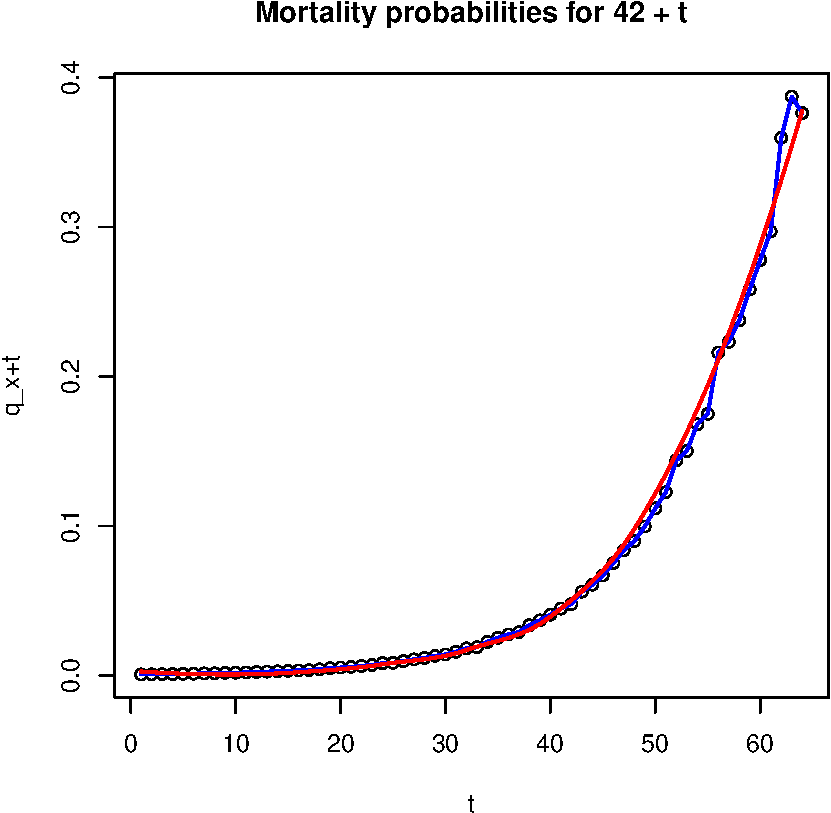
\includegraphics{LifeCon_files/figure-latex/NewlyUnderwrittenLifeQxa-1} 

}

\caption{\textbf{Mortality probabilities for a 42-year-old non-smoking male with a BMI of 28 and a blood pressure of 127.}}\label{fig:NewlyUnderwrittenLifeQxa}
\end{figure}

We notice that the raw mortality probabilities (dots and blue curve) show some irregularities, so we also prvovide a smoothed version based on a local regression fit (via \texttt{loess}). The survival function and the mortality probabilities can be used for actuarial calculations.

Life insurance policies have a complex benefit structure that requires knowledge upon the probability of paying the benefits besides many other risk modeling parameters. Policy pricing, meeting the regulatory requirements, and understanding the life portfolio risk performance are all actuarial evaluations that rely on these risk modeling parameters. Mortality risk plays an important role for all of these. In the coming chapters, we discuss how -- given (an estimate of) the distribution of the future lifetime random variable \(T_{\bf{x}}\) -- we can perform these evaluations. In principle, any model discussed in this chapter can be used.

As we have seen, models of different degrees of sophistication are possible. What approach is adequate depends on the application in view. For instance, for statutory calculations governed by insurance regulation, often certain life tables are mandated that only account for a limited set of factors (sex, smoking status, etc.). In contrast, when pricing term life insurance policies, the underwriting process can be intricate and resulting information can be leveraged to quote a premium that closely reflects the adopted risk.

\hypertarget{notes-and-comments}{%
\section{Notes and Comments}\label{notes-and-comments}}

Reference to Survival analysis textbooks

\hypertarget{Sec:LifeTableRecursive}{%
\section{Appendix 2A. Life Table: Recursive Calculations}\label{Sec:LifeTableRecursive}}

Actuaries and other analysts have found \emph{life tables} to be useful in interpreting mortality patterns for many years. Origins of life tables can be traced back to Edmund Halley's paper entitled, ``An estimate of the degrees of the mortality of mankind, drawn from various tables of births and funerals in the city of Breslau,'' published in 1693. Some scholars attribute this paper as marking the birth of actuarial science.

As introduced in \emph{Section 2.4}, a life table is based on the quantities \(l_x = radix \times S_a(x)\) where \(S_a(\cdot)\) is the survival function for a life aged \(a\). In this expression, \(a\) is the starting age of the table and \(radix\) is a constant generally taken so that \(l_a\) is a large round number. With this choice, we interpret \(l_x\) to be the ``number living'' at age \(x\).

\protect\hyperlink{tab:2A1}{Table 2A.1} shows life tables for female and male Indonesians. Here, each radix, one for females and one for males, is chosen so that there are 100,000 people alive at age \(a=20\). Also from \protect\hyperlink{tab:2A1}{Table 2A.1}, you will see that the mortality distribution is given in terms of (integral) values of \(x\); such a choice is common in life tables as is other regular successive values, e.g., quinquennial for five year values.

With a table of successive values, many interesting recursive expressions are available. To begin, we can define the change \(d_x = l_x - l_{x+1}\) that we interpret as the ``number dying'' between ages \(x\) and \(x+1\). These changes allow us to express life table quantities \(l_x\) and \(d_x\) in terms of one-year death rates, \(q_x\), as follows. Recall that \(q_x = 1 - S_0(x+1)/S_0(x) = 1 - S_a(x+1)/S_a(x)\) and so

\[
\frac{d_x}{l_x} = \frac{l_x - l_{x+1}}{l_x} = \frac{radix}{radix}\frac{S_a(x) - S_a(x+1)}{S_a(x)} = q_x .
\]

From this we can use life table quantities \(l_x\) and \(d_x\) to calculate one-year death rates, \(q_x\). We can also reverse the process. That is,
starting with one-year death rates as inputs, we can calculate life table entries recursively using \(l_{x+1} = l_x - l_x q_x = l_x p_x\) for \(x=a, a+1, \ldots\). Thus, for example, in \protect\hyperlink{tab:2A1}{Table 2A.1}, with \(x=20\), we have \(l_{21} = l_{20} - l_{20} q_{20} = (100000)(1 - 0.000340) = 99966\). For readers familiar with spreadsheet methods, click on a few cells in \protect\hyperlink{tab:2A1}{Table 2A.1} to see the recursive definition of table entries.

Later chapters on life contingent benefits will highlight recursive calculations. To foreshadow this, consider the curtate life expectancy introduced in \emph{Section 2.4}. An easy calculation (that the reader should verify) shows the recursive expression

\[
e_x = \sum_{k=1}^{\infty} ~ {~}_k p_x 
= p_x (1 + e_{x+1}) .
\]

The \(e_x\) columns in \protect\hyperlink{tab:2A1}{Table 2A.1} utilize this relationship. To visualize these entries, Figure \ref{fig:IndonesianLifeTablePlot} compares female to male life expectancies for the Indonesian data. Here, we see that females have a higher life expectancy at each age. The difference is greatest at the first age of the table \(a=20\) which is 61.06 - 55.46 = 5.60.

\textbf{On Your Own.} The Indonesian mortality data were retrieved from the \href{https://mort.soa.org}{Mortality and Other Rate Tables} database sponsored by the Society of Actuaries. This database contains mortality (and other) rates from scores of countries. You will enjoy downloading them and comparing mortality experiences across the globe.

Table 2A.1. \textbf{Indonesian Life Table}

\hypertarget{spreadsheetLC2A1}{}

Export this spreadsheet as CSV



\begin{figure}

{\centering 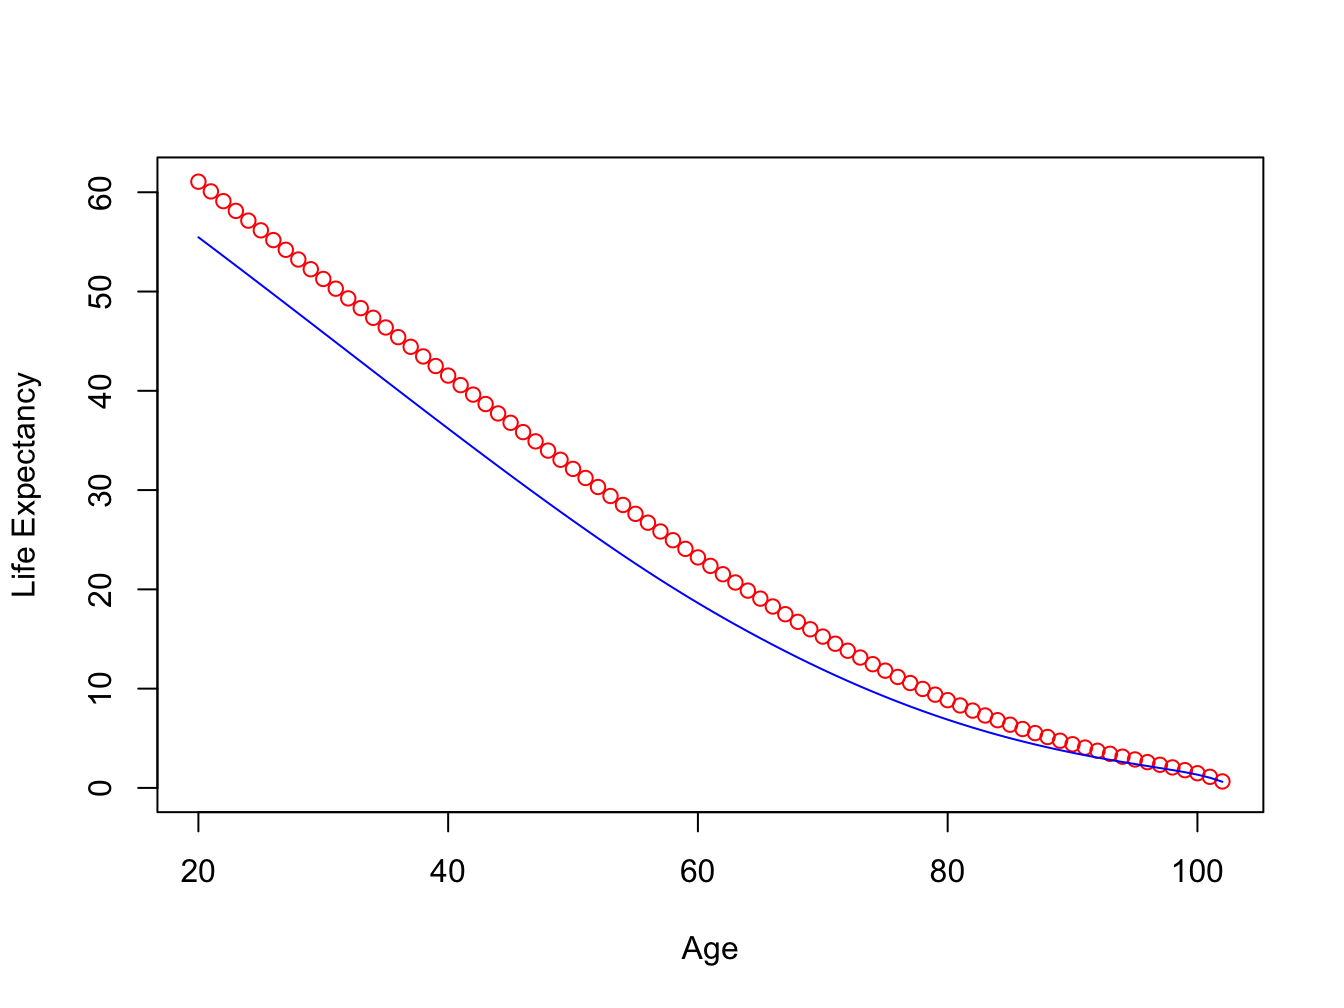
\includegraphics[width=0.75\linewidth]{LifeCon_files/figure-latex/IndonesianLifeTablePlot-1} 

}

\caption{\textbf{Indonesian Life Expectancies.} Female life expectancies are given in the red open symbols, males are represented with the blue solid line.}\label{fig:IndonesianLifeTablePlot}
\end{figure}

\textbf{On Your Own.} Try a few interactive calculations using \texttt{R}.

eyJsYW5ndWFnZSI6InIiLCJzYW1wbGUiOiJJbmRMaWZlVGFibGUgPC0gcmVhZC5jc3YoXCJodHRwczovL3Jhdy5naXRodWJ1c2VyY29udGVudC5jb20vT3BlbkFjdFRleHREZXYvTGlmZUNvbi9tYXN0ZXIvRGF0YS9JbmRvbmVzaWFuTGlmZVRhYmxlTm9Gb3JtdWxhLmNzdlwiLCBoZWFkZXIgPSBGKVxuY29sbmFtZXMoSW5kTGlmZVRhYmxlKSA8LSBjKFwiQWdlXCIsXCJGZW1hbGUucXhcIixcIkZlbWFsZS5seFwiLFwiRmVtYWxlLmR4XCIsXCJGZW1hbGUuZXhcIixcIk1hbGUucXhcIixcIk1hbGUubHhcIixcIk1hbGUuZHhcIixcIk1hbGUuZXhcIilcbnN1bW1hcnkoSW5kTGlmZVRhYmxlKVxucGxvdChJbmRMaWZlVGFibGUkQWdlLEluZExpZmVUYWJsZSRGZW1hbGUuZXgsIHhsYWI9XCJBZ2VcIix5bGFiPVwiTGlmZSBFeHBlY3RhbmN5XCIsIGNvbD1cInJlZFwiKVxubGluZXMoSW5kTGlmZVRhYmxlJEFnZSxJbmRMaWZlVGFibGUkTWFsZS5leCwgY29sPVwiYmx1ZVwiKSJ9

\hypertarget{C:NotationConventionLC}{%
\chapter{Appendix: Conventions for Notation}\label{C:NotationConventionLC}}

\emph{Chapter Preview}. \emph{Life Contingencies} employs widely accepted statistical concepts and tools. Thus, the notation should be consistent with standard usage employed in probability and mathematical statistics. See, for example, \citep{halperin1965recommended} for a description of one standard.

\hypertarget{S:NC:ActSymbols}{%
\section{Actuarial Notation}\label{S:NC:ActSymbols}}

Here is a list of commonly used actuarial symbols and functions, including the latex code that we use to generate them.

\hypertarget{life-table-symbols}{%
\subsection{Life Table Symbols}\label{life-table-symbols}}

\[
{\small
\require{enclose}
\begin{array}{cll}  \hline
\textbf{Symbol} & \textbf{Latex code} & \textbf{Description} \\
\hline
\ell_{x} & \verb|\| \tt{ell}\_\{\tt{x}\} & \text{Expected number of lives at age } x \\
\ell_{[x]} & \backslash\tt{ell}\_\{ [\tt{x}]\} & \text{Expected number of lives at select age } x \\
_{t}p_{x} &    ~ \_\{ \tt{t} \} \tt{p} \_ \{\tt{x}\} & \text{Probability that a life aged } x \text{ survives }t \text{ years} \\
_{t}p_{[x]} &    ~ \_\{ \tt{t} \} \tt{p} \_ \{ [\tt{x}]\}\} & \text{Probability that a select life aged } x \text{ survives }t \text{ years} \\
\mathring{e}_{x} & \backslash\tt{mathring\{e\}} \_ \{ x\} & \text{Complete expectation of life at age } x \\
\mathring{e}_{x:{\enclose{actuarial}{n}}} & \backslash\tt{mathring\{e\}} \_ \{ x:\{\backslash enclose\{actuarial\}\{n\}\}\} & \text{Complete expectation of life at age } x \text{ for the next } n \text{ years} \\
\hline
\end{array}
}
\]

\hypertarget{Sec:LifeInsSymbols}{%
\subsection{Life Insurance Symbols}\label{Sec:LifeInsSymbols}}

\[
{\small
\begin{array}{cll}  \hline
\textbf{Symbol} & \textbf{Latex code} & \textbf{Description} \\
\hline
A_{x} &    \tt{A} \_ \{\tt{x}\} & \text{APV of a discrete whole life insurance to } (x) \\
\bar{A}_{x} &    \backslash \tt{bar} \{\tt{A}\} \_ \{\tt{x}\} & \text{APV of a continuous whole life insurance to } (x) \\
A^{(m)}_{x} &    \tt{A} \verb|^| \tt{\{(m)\}}\_ \{\tt{x}\} & \text{APV of a whole life insurance payable at end of } m\text{-th of the year of death of } (x) \\
_{n}E_{x} &    ~ \_\{ \tt{n} \} \tt{E} \_ \{\tt{x}\} & \text{APV of an } n\text{-year pure endowment to } (x) \\
{A}_{x:\enclose{actuarial}{n}}^{\quad 1} & \{\tt{A}\} \_ \{ x:\{\backslash enclose\{actuarial\}\{n\}\}\} \verb|^| \{\backslash \tt{quad} \ 1\} & \text{APV of an } n\text{-year term insurance to } (x)  \\
{A}_{x:{\enclose{actuarial}{n}}} & \{\tt{A}\} \_ \{ x:\{\backslash enclose\{actuarial\}\{n\}\}\} & \text{APV of an } n\text{-year endowment insurance to } (x) \\
_{n|}{A}_{x} & ~ \_\{ \tt{n|} \} \{\tt{A}\_\{x\}\} & \text{APV of an } n\text{-year deferred life insurance to } (x) \\
{A}_{x:\enclose{actuarial}{n}}^{\space 1} & \{\tt{A}\} \_ \{ x:\{\backslash enclose\{actuarial\}\{n\}\}\} \verb|^| \{\backslash \tt{space} \ 1\} & \text{APV of an } n\text{-year term insurance to } (x)  \\
\hline
\end{array}
}
\]

\hypertarget{Sec:LifeAnnSymbols}{%
\subsection{Annuity Certain and Life Annuity Symbols}\label{Sec:LifeAnnSymbols}}

\[
{\small
\begin{array}{cll}  \hline
\textbf{Symbol} & \textbf{Latex code} & \textbf{Description} \\
\hline
a_{\enclose{actuarial}{n}} & \tt{a}\_\{\backslash \tt{enclose}\{actuarial\}\{\tt{n}\}\} & n\text{-year annuity certain-immediate} \\
\ddot{a}_{\enclose{actuarial}{n}} & \backslash\tt{ddot}\_\{\tt{a}\_\{\backslash \tt{enclose}\{actuarial\}\{\tt{n}\}\} & n\text{-year annuity certain-due} \\
\ddot{a}^{(m)}_{\enclose{actuarial}{n}} & \backslash\tt{ddot} \verb|^| \tt{\{(m)\}}\_\{\tt{a}\_\{\backslash \tt{enclose}\{actuarial\}\{\tt{n}\}\} & n\text{-year annuity certain-due payable } m\text{-thly}  \\
_{m|}\ddot{a}_{\enclose{actuarial}{n}} & ~ \_\{ \tt{m|} \} \backslash\tt{ddot}\_\{\tt{a}\_\{\backslash \tt{enclose}\{actuarial\}\{\tt{n}\}\} & m\text{-year deferred } n\text{-year annuity certain-due} \\
a_{x} & \tt{a}\_\{x\} & \text{APV of a whole life annuity immediate to } (x) \\
\ddot{a}_{x} & \backslash\tt{ddot}\{\tt{a}\}\_\{x\} & \text{APV of a whole life annuity due to } (x) \\
a^{(m)}_{x} & \tt{a} \verb|^| \tt{\{(m)\}}\_\{x\} & \text{APV of a life annuity immediate to } (x) \text{ payable } m\text{-thly} \\
\ddot{a}^{(m)}_{x} & \backslash\tt{ddot}\{\tt{a}\} \verb|^| \tt{\{(m)\}}\_\{x\} & \text{APV of a life annuity due to } (x) \text{ payable } m\text{-thly} \\
_{n|}\ddot{a}_{x} & ~ \_\{ \tt{n|} \} \backslash\tt{ddot}\_\{\tt{a}\_\{x\}\} & \text{APV of an } n\text{-year deferred life annuity due to } (x) \\
\ddot{a}_{x:{\enclose{actuarial}{n}}} & \backslash\tt{ddot\{a\}} \_ \{ x:\{\backslash enclose\{actuarial\}\{n\}\}\} & \text{APV of an } n\text{-year life annuity due to } (x) \\
\ddot{a}^{(m)}_{x:{\enclose{actuarial}{n}}} & \backslash\tt{ddot\{a\}} \verb|^| \tt{\{(m)\}} \_ \{ x:\{\backslash enclose\{actuarial\}\{n\}\}\} & \text{APV of an } n\text{-year life annuity due to } (x) \text{ payable } m\text{-thly} \\
\hline
\end{array}
}
\]

Not sure if necessary to say \(APV\) (actuarial present value)

\hypertarget{C:NotConv:Halo}{%
\section{Halo System}\label{C:NotConv:Halo}}



\begin{figure}

{\centering 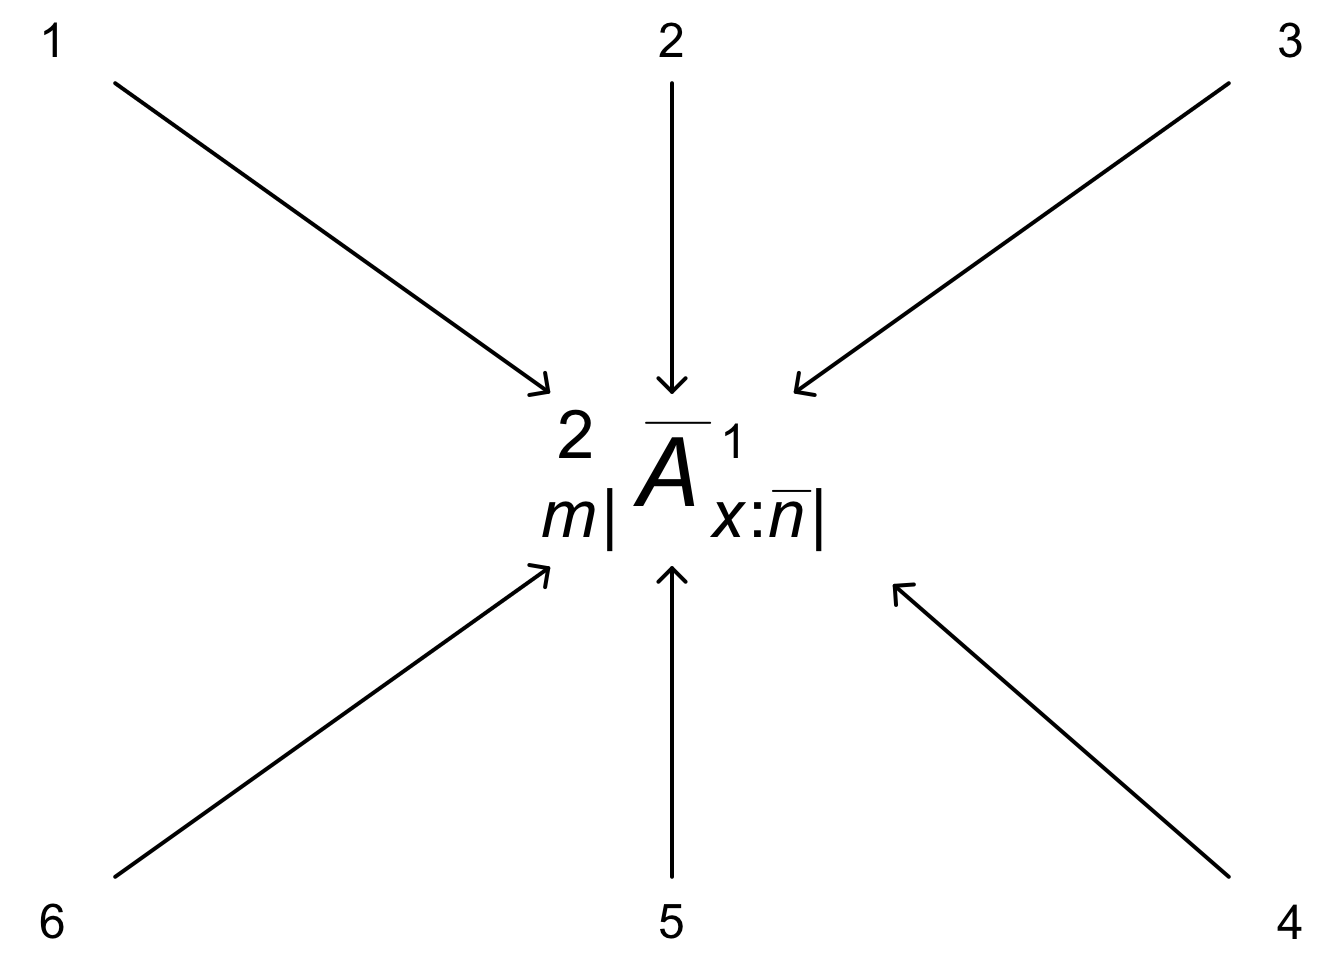
\includegraphics[width=0.5\linewidth]{LifeCon_files/figure-latex/Halo1a-1} 

}

\caption{\textbf{Halo System: Example of an Actuarial Symbol}. \emph{Source}: This is adapted from the \emph{Wikipedia} page \href{https://en.wikipedia.org/wiki/Actuarial_notation}{Actuarial Notation}.}\label{fig:Halo1a}
\end{figure}

\begin{center}\rule{0.5\linewidth}{0.5pt}\end{center}

\newpage

\textbf{Legend:}

\begin{itemize}
\tightlist
\item
  1 - the ``2'' means double the force of interest
\item
  2 - the bar implies continuous, or payments at the moment of death. No bar, or blank, signifies payment at the end of the year.
  For annuities, could use a double dot that signifies payments at the beginning of the year.
\item
  3 - the ``1'' denotes a temporary, or term, payment. Paid if \(x\) within \(n\) years
\item
  4 - contract issued to a life aged \(x\) and lasts for at most \(n\) years.
\item
  5 - the ``A'' signifies it is an insurance (``assurance'') contract. Could also be a lower case \(a\) that would signify an annuity contract.
\item
  6 - deferred \emph{m} years
\end{itemize}

\textbf{Note:} It is sometimes helpful to put a space before the pre-subscript like \(\frac{\ell_{[x]+t}}{\ell_{[x]}} = ~_{t}p_{[x]}\). Else you get this awkward \(\frac{\ell_{[x]+t}}{\ell_{[x]}} = _{t}p_{[x]}\).

\[
Y =
 \begin{cases}
 1 + v + v^2 + \cdots + v^K = \ddot{a}_{\enclose{actuarial}{K+1}}, K=0,1,\ldots,n-1 \\
 1 + v + v^2 + \cdots + v^{n-1} = \ddot{a}_{\enclose{actuarial}{n}}, K \ge n
 \end{cases}
\]
\textbf{Note.}

\begin{itemize}
\tightlist
\item
  For the \texttt{html} version of the text, we are using the \href{}{STACK} system; in particular, see their \href{https://stack-demo.maths.ed.ac.uk/demo/question/type/stack/doc/doc.php/Authoring/Actuarial.md}{actuarial notation} page.
\item
  This does not appear to work for the \texttt{pdf} version, at least with R-Studio. The latex package \href{https://ctan.org/pkg/actuarialsymbol?lang=en}{actuarialangle} provides a substitute. To make this happen, in our latex header .tex page, we have the following bit of code
\end{itemize}

\begin{verbatim}
%  Something for the Actuarial Angle package
\usepackage{actuarialangle}
\newcommand{\enclose}[1]{\actuarialangle} 
\end{verbatim}

\hypertarget{S:NC:General}{%
\section{General Conventions}\label{S:NC:General}}

\begin{itemize}
\tightlist
\item
  Random variables are denoted by upper-case italicized Roman letters, with \(X\) or \(Y\) denoting a claim size variable, \(N\) a claim count variable, and \(S\) an aggregate loss variable. Realizations of random variables are denoted by corresponding lower-case italicized Roman letters, with \(x\) or \(y\) for claim sizes, \(n\) for a claim count, and \(s\) for an aggregate loss.
\item
  Probability events are denoted by upper-case Roman letters, such as \(\Pr(\mathrm{A})\) for the probability that an outcome in the event `'A'' occurs.
\item
  Cumulative probability functions are denoted by \(F(z)\) and probability density functions by the associated lower-case Roman letter: \(f(z)\).
\item
  For distributions, parameters are denoted by lower-case Greek letters. A caret or `'hat'' indicates a sample estimate of the corresponding population parameter. For example, \(\hat{\beta}\) is an estimate of \(\beta\) .
\item
  The arithmetic mean of a set of numbers, say, \(x_1, \ldots, x_n\), is usually denoted by \(\bar{x}\); the use of \(x\), of course, is optional.
\item
  Use upper-case boldface Roman letters to denote a matrix other than a vector. Use lower-case boldface Roman letters to denote a (column) vector. Use a superscript prime '`\(\prime\)'' for transpose. For example, \(\mathbf{x}^{\prime} \mathbf{A} \mathbf{x}\) is a quadratic form.
\item
  Acronyms are to be used sparingly, given the international focus of our audience. Introduce acronyms commonly used in statistical nomenclature but limit the number of acronyms introduced. For example, \emph{pdf} for probability density function is useful but \emph{GS} for Gini statistic is not.
\end{itemize}

\hypertarget{S:NC:Abbreviations}{%
\section{Abbreviations}\label{S:NC:Abbreviations}}

Here is a list of abbreviations that we adopt. We italicize these acronyms. For example, we can discuss the goodness of fit in terms of the \emph{AIC} criterion.

\[
\begin{array}{ll} \hline
\textbf{Symbol} & \textbf{Description} \\
\hline
AIC & \text{Akaike information criterion} \\
BIC & \text{(Schwarz) Bayesian information criterion} \\
cdf & \text{cumulative distribution function} \\
df & \text{degrees of freedom} \\
iid & \text{independent and identically distributed} \\
GLM & \text{generalized linear model} \\
mle & \text{maximum likelihood estimate/estimator}\\
ols & \text{ordinary least squares} \\
pdf & \text{probability density function} \\
pmf & \text{probability mass function} \\ \hline
\end{array}
\]

\hypertarget{S:NC:StatSymbols}{%
\section{Common Statistical Symbols and Operators}\label{S:NC:StatSymbols}}

Here is a list of commonly used statistical symbols and operators, including the latex code that we use to generate them (in the parens).

\[
\begin{array}{cl}  \hline
\textbf{Symbol} & \textbf{Description} \\
\hline
I(\cdot) & \text{binary indicator function (}I\text{). For example, }I(A) \text{ is one if an outcome in event} \\
& \ \ \ \ \  A \text{ occurs and is 0 otherwise.} \\
\Pr(\cdot) & \text{probability }(\backslash{\tt{Pr}}) \\
\mathrm{E}(\cdot)  & {\text{expectation operator }} (\backslash{\tt{mathrm\{E\}}}). {\text{ For example, }} \mathrm{E}(X)=\mathrm{E}~X {\text{ is the }} \\
& \ \ \ \ \ {\text{expected value of the random variable }}X,{\text{ commonly denoted by }}\mu. \\
\mathrm{Var}(\cdot)  & \text{variance operator }(\backslash{\tt{mathrm\{Var\}}}). \text{ For example, } \mathrm{Var}(X)=\mathrm{Var}~X\text{ is the} \\
& \ \ \ \ \  \text{ variance of the random variable } X, \text{commonly denoted by } \sigma^2. \\
\mu_k = \mathrm{E}~X^k & \text{kth moment of the random variable X. For }k\text{=1, use }\mu = \mu_1. \\
\mathrm{Cov}(\cdot,\cdot)  & \text{covariance operator } (\backslash{\tt{mathrm\{Cov\}}}).\text{ For example, } \\
& \ \ \ \ \ \mathrm{Cov}(X,Y)=\mathrm{E}\left\{(X -\mathrm{E}~X)(Y-\mathrm{E}~Y)\right\}  =\mathrm{E}(XY) -(\mathrm{E}~X)(\mathrm{E}~Y)\\
& \ \ \ \ \  \text{ is the covariance between random variables }X\text{ and }Y. \\
\mathrm{E}(X | \cdot)  & \text{conditional expectation operator. For example, }\mathrm{E}(X |Y=y) \text{ is the}\\
& \ \ \ \ \   \text{ conditional expected value of a random variable }X\text{ given that }\\
& \ \ \ \ \   \text{ the random variable }Y\text{ equals y. }\\
\Phi(\cdot) & \text{standard normal cumulative distribution function }(\backslash{\tt{Phi}})\\
\phi(\cdot) & \text{standard normal probability density function }(\backslash{\tt{phi}})\\
\sim & \text{means is distributed as }(\backslash{\tt{sim}}). \text{ For example, }X\sim F \text{ means that the } \\
& \ \ \ \ \  \text{random variable } X \text{ has distribution function }F. \\
se(\hat{\beta}) & \text{standard error of the parameter estimate }\hat{\beta} ~ (\backslash{\tt{hat\{}}\backslash{\tt{beta\}}}), \text{ usually }\\
& \ \ \ \ \  \text{ an estimate of the standard deviation of }\hat{\beta},\text{ which is }\sqrt{Var(\hat{\beta})}. \\
H_0 &  \text{null hypothesis} \\
H_a \text{ or }H_1 & \text{alternative hypothesis} \\
\hline
\end{array}
\]

\hypertarget{S:NC:Symbols}{%
\section{Common Mathematical Symbols and Functions}\label{S:NC:Symbols}}

Here is a list of commonly used mathematical symbols and functions, including the latex code that we use to generate them (in the parens).

\[
\begin{array}{cll}
\hline
\textbf{Symbol} & \textbf{Latex code} & \textbf{Description} \\
\hline
\equiv & \backslash\tt{equiv} & \text{identity, equivalence} \\
\implies  & \backslash\tt{implies} & \text{implies} \\
\iff  & \backslash\tt{iff} & \text{if and only if} \\
\to, \longrightarrow & \backslash\tt{to}, \backslash\tt{longrightarrow} & \text{converges to} \\
\mathbb{N} & \backslash\tt{mathbb\{N\}} & \text{natural numbers }1,2,\ldots \\
\mathbb{R} & \backslash\tt{mathbb\{R\}} & \text{real numbers} \\
\in        & \backslash\tt{in} & \text{belongs to} \\
\notin     & \backslash\tt{notin} & \text{does not belong to} \\
\subseteq  & \backslash\tt{subseteq} & \text{is a subset of} \\
\subset    & \backslash\tt{subset} & \text{is a proper subset of} \\
\cup       & \backslash\tt{cup} & \text{union} \\
\cap       & \backslash\tt{cap} & \text{intersection} \\
\emptyset  & \backslash\tt{emptyset} & \text{empty set} \\
A^{c}      &  & \text{complement of }A   \\
g*f        &  & \text{convolution }(g*f)(x)=\int_{-\infty}^{\infty}g(y)f(x-y)dy \\
\exp       & \backslash\tt{exp} & \text{exponential} \\
\log       & \backslash\tt{log} & \text{natural logarithm }\\
\log_a     &  & \text{logarithm to the base }a \\
!          &  & \text{factorial} \\
\text{sgn}(x) & \backslash\tt{sgn} & \text{sign of x} \\
\lfloor x\rfloor & \backslash\tt{lfloor}, \backslash\tt{rfloor} & \text{integer part of x, that is, largest integer }\leq x \\
|x|        &  & \text{absolute value of scalar }x \\
\varGamma(x) & \backslash\tt{varGamma} & \text{gamma (generalized factorial) function},\\
           &  & \text{satisfying }\varGamma(x+1)=x\varGamma(x) \\
B(x,y)     &  & \text{beta function, }\varGamma(x)\varGamma(y)/\varGamma(x+y) \\
\hline
\end{array}
\]

\hypertarget{further-readings}{%
\section{Further Readings}\label{further-readings}}

To make connections to other literatures, see \citep{abadir2002notation} \url{http://www.janmagnus.nl/misc/notation.zip} for a summary of notation from the econometrics perspective. This reference has a terrific feature that many latex symbols are defined in the article. Further, there is a long history of discussion and debate surrounding actuarial notation; see \citep{boehm1975thoughts} for one contribution.

Time taken for this draft of the book: 0.71 minutes.

  \bibliography{References/LDAReference2020A.bib}

\end{document}
